% \chapter{Experiments and Results}


% % \newpage

% \section*{Introduction}
% \label{sec:introduction}

% This chapter presents a comprehensive empirical evaluation of our proposed Learning-Informed Masking Framework. As established in the previous chapter, our work builds upon the Multi-Agent Masked Auto-Encoder (MA2E) architecture, a powerful method for inferring global information from local observations. However, we identified a key limitation in the original MA2E: its reliance on a policy-agnostic, random masking strategy. This approach creates a disconnect between the self-supervised reconstruction task and the primary reinforcement learning objective.

% The central thesis of our work is that for optimal performance, these two tasks must be dynamically aligned. This chapter aims to empirically validate our core hypothesis: that using an agent's own training dynamics to guide the representational learning process yields a more efficient and effective learning curriculum. Specifically, we will test whether our proposed Learning-Informed Masking—which leverages the Temporal Difference (TD) error to focus the autoencoder's attention on the most uncertain agents—yields superior performance over the original random masking approach.

% To validate this, we will benchmark our framework directly against the baseline original MA2E. This focused comparison is designed to isolate and measure the impact of our intelligent masking strategy. The experiments are conducted on the challenging StarCraft Multi-Agent Challenge (SMAC) \parencite{smac},
% % and its more demanding successor, SMACv2 \parencite{smacv2},
% to test the limits of coordination and generalization under partial observability.
\chapter{Experiments and Results}

\section*{Introduction}
\label{sec:introduction_ch5} 

This chapter provides a comprehensive empirical validation of our proposed Learning-Informed Masking Framework ($LI-{MA}^2E$). The primary objective is to demonstrate its superiority over the baseline ${MA}^2E$ framework, which utilizes a random masking strategy. To achieve this, we conduct a series of rigorous experiments on a diverse suite of challenging scenarios from the StarCraft Multi-Agent Challenge (SMAC).

The chapter is structured to present a complete scientific narrative. We begin by detailing our methodical investigation into several candidate scoring functions, showing the iterative process that led to the selection of our final, most effective approach: Adaptive Mean TD-Error Thresholding. Following this, we present a comprehensive performance evaluation of this optimized framework, structured to answer three core research questions regarding its effectiveness in \textit{task completion} (via win rate), its ability to produce \textit{high-quality policies} (via mean test return), and the underlying \textit{learning dynamics} that drive its success (via TD-error).

Ultimately, this chapter will provide robust, multi-faceted evidence to support our central thesis that a learning-informed masking curriculum is superior to a random one in complex, cooperative multi-agent tasks.

\section{Experimental Details}
In this section, we introduce the environments used in the experiments, the baseline algorithm, and the hyperparameters and computational resources. Experiments are carried out on an NVIDIA RTX A5000 GPU (24.6\,GB VRAM) and an Intel\textregistered\ Xeon\textregistered\ W-2235 CPU (6-core, 12-thread), with 32\,$\mathrm{GB}$ DDR4 RAM and CUDA 12.4 support. All algorithms are implemented based on the open-source framework pymarl2\footnote{From: \url{https://github.com/hijkzzz/pymarl2}}  \parencite{pymarl2}, which is an augmented version of pymarl\footnote{From: \url{https://github.com/oxwhirl/pymarl}}. Both are licensed under Apache License 2.0. 
 All the experiments are conducted during a minimum $1 \times 10^6$ time steps.
 %, and we report \textit{the average win rates} with the shaded standard error random seeds.

\subsection{Environments}
\subsubsection{SMAC}

The StarCraft Multi-Agent Challenge (SMAC) \parencite{smac} is one of the benchmarks widely utilized in research to evaluate MARL algorithms. In SMAC, units from the strategy video game StarCraft engage in combat in diverse scenarios. The objective is for multiple agents to collaborate to defeat the enemy forces. The scenarios are categorized by difficulty  Table~\ref{tab:smac_senarios_part1} and Table~\ref{tab:smac_senarios_part2}.

\noindent\textbf{Note:} The objective in all scenarios in Table~\ref{tab:smac_scenarios_used} is to defeat all enemy units by employing the strategy noted in the \textbf{Type} column.

\begin{table}[H]
\centering

\renewcommand{\arraystretch}{1.6} 

\begin{tabular}{ccccc}
\hline
\textbf{Scenario} & \textbf{Difficulty} & \textbf{Ally Units} & \textbf{Enemy Units} & \textbf{Primary Micro-Trick} \\
\hline
3s\_vs\_3z & EASY & 3 Stalkers & 3 Zealots & Kiting \\
\hline
3s\_vs\_4z & MEDIUM & 3 Stalkers & 4 Zealots & Kiting \\
\hline
3s\_vs\_5z & HARD & 3 Stalkers & 5 Zealots & Kiting \\
\hline
3m & EASY & 3 Marines & 3 Marines & Focus Fire \\
\hline
8m & MEDIUM & 8 Marines & 8 Marines & Focus Fire \\
\hline
\end{tabular}
\caption{A detailed description of the SMAC scenarios used in the experiment.}
\label{tab:smac_scenarios_used}
\end{table}
% \subsubsection{SMACv2}

% SMACv2 \parencite{smacv2}  was proposed to address the shortcomings of the original SMAC, particularly its lack of stochasticity and meaningful partial observability (for more details \parencite{smacv2_review}). Therefore, SMACv2 differs from SMAC in three main aspects:

% \begin{enumerate}
%     \item \textbf{Random Unit Composition:} In SMAC, the units in each matchup are fixed, whereas in SMACv2, different unit types are randomly generated for each episode based on probabilities.
%     \item \textbf{Probabilistic Observation:} In SMACv2, if one agent observes an enemy, other nearby agents may not immediately identify the same enemy, even if it is within their observation range. This contrasts with SMAC, where an enemy observed by one agent is simultaneously visible to all other agents.
%     \item \textbf{Randomized Spawn Locations:} The starting positions for units are randomized and determined by one of two types: \texttt{surround} or \texttt{reflect}. \texttt{surround} places allied units in a formation encircling the enemy, while \texttt{reflect} involves a head-on confrontation.

% \begin{figure}[h]
%     \centering
   
        
%     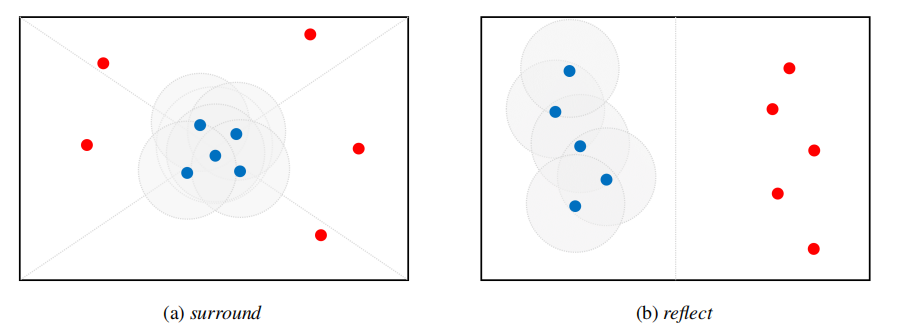
\includegraphics[width= 0.7\linewidth]{img_pfe/start_pos_smacv2.PNG}
 
  
%                 \caption{Two different types of start positions in SMACv2.(Adapted from \parencite{ma2e})}
%         \label{fig:start_pos_smacv2}
% \end{figure}
    
% \end{enumerate}

\subsection{Baseline Algorithm}

Our experiments are designed to isolate the impact of our Learning-Informed masking strategy. Therefore, the baseline for all comparisons is the \textbf{original ${MA}^2E$ architecture}, which utilizes a \textbf{random masking strategy} during training. Both our proposed framework and the baseline are integrated into the \textbf{\ac{QMIX}} algorithm.


\subsection{Hyperparameters}

To ensure a controlled and fair comparison, our proposed framework (\textbf{QMIX + $LI-{MA}^2E$}) and the baseline (\textbf{QMIX + ${MA}^2E$}) share the same core network architecture and hyperparameters. The parameters for the QMIX backbone algorithm are listed in Table \ref{tab:qmix_hyperparams}, and the parameters for the $LI-{MA}^2E$ and ${MA}^2E$ module are listed in Table \ref{tab:ma2e_hyperparams}. These values were used for all experimental runs.

\begin{table}[H]
\centering

\renewcommand{\arraystretch}{1.5} 
\begin{tabular}{lc} 
\hline
\textbf{Hyperparameter} & \textbf{Value} \\
\hline 
Optimizer & Adam \\
Learning Rate (lr) & 0.001 \\
Batch Size & 128 \\
Replay Buffer Size & 1000 \\
Discount Factor ($\gamma$) & 0.99 \\
TD-Lambda ($\lambda$) & 0.6 \\
Epsilon Anneal Steps & 100000 \\
RNN Hidden Dimension & 128 \\
QMIX Mixing Embedding Dimension & 32 \\
\hline
\end{tabular}
\caption{Hyperparameters for the QMIX Backbone Algorithm.}
\label{tab:qmix_hyperparams}
\end{table}

\begin{table}[H]
\centering

\renewcommand{\arraystretch}{1.5} 
\begin{tabular}{lc} 
\hline
\textbf{Hyperparameter} & \textbf{Value} \\
\hline 
Input Trajectory Length & 5 \\
Batch Size & 32 \\
Input Embedding Dimension & 24 \\
Number of Attention Heads & 4 \\
Number of Encoder Layers & 3 \\
Number of Decoder Layers & 2 \\
Steps for Fine-Tuning & 500 \\
Pre-training Threshold & 0.015 \\
\hline
\end{tabular}
\caption{Hyperparameters for the \textbf{$LI-{MA}^2E$} and \textbf{${MA}^2E$} Module.}
\label{tab:ma2e_hyperparams}
\end{table}
\section{Developing the Learning-Informed Masking Score}
% \section{Comparative Analysis of Agent Scoring Methods}
\label{sec:scoring_methods}

The core of our \textbf{$LI-{MA}^2E$ framework} is the ability to intelligently mask \textit{poorly performing} agents. However, defining \textit{poor performance} is not simple. To determine the most effective metric, we designed and empirically evaluated several candidate scoring methodologies, each with a unique theoretical motivation. This section details our investigation into these scoring methods, their underlying rationales, their limitations, and the results that led to our final design choice.
\subsection{Method 1: TD-error with Exponential Moving Average (EMA)}
\label{subsec:ema_method}


Our initial approach to identifying poorly performing agents was to track their long-term performance stability. We chose the TD-error as the fundamental metric for this task. The TD-error, generated during the training of the backbone algorithm, represents the "surprise" or prediction error of an agent's value function for a given transition. 

\paragraph{why \ac{TD} error as metric  ?} 
TD error quantifies the difference between the predicted value of a state-action pair and a better-informed estimate based on the next state:

\begin{equation}
    \delta_t = 
    \underbrace{\left(r_{t+1} + \gamma \max_{a'} Q(s_{t+1}, a')\right)}_{\text{TD target}} 
    - Q(s_t, a_t)
    \label{eq:td_error}
\end{equation}

\begin{itemize}
    \item $r_{t+1}$: The immediate reward received after taking action $a_t$ in state $s_t$.
    \item $\gamma$: The discount factor, controlling the weight of future rewards.
    \item $Q(s_{t+1}, a')$: The estimated value of the next state $s_{t+1}$ under action $a'$, over which we take the maximum (greedy choice) to estimate the best possible future return.
    \item TD target: represents a better-informed estimate of the return assuming the agent acts optimally from $s_{t+1}$ onward.

\end{itemize}

A high absolute TD error ($|\delta_t|$) indicates that the agent's current estimate is significantly inaccurate: highlighting a weakness in its value function and suggesting that this region of the state-action space reflects \textit{poor learning progress}.



Our first hypothesis was that smoothing this error signal over time using an \ac{EMA} would provide a stable measure of an agent's overall learning quality, filtering out noisy, single-step errors. The \ac{EMA} is updated recursively, giving more weight to recent errors while still retaining information from the past. The formula is:
\begin{equation}
    \text{EMA}_t = \alpha \cdot |\delta_t| + (1 - \alpha) \cdot \text{EMA}_{t-1}
    \label{eq:ema}
\end{equation}
where $\alpha$ is the decay rate, determining the balance between new and historical errors.

\paragraph{Implementation}
The implementation is tightly coupled with the overall training loop. Our framework follows a periodic fine-tuning schedule: the QMIX agent policies are trained multiple times, and during this time, all TD errors generated are continuously collected and stored in a large buffer, paired with their respective agent IDs. When it is time to fine-tune the MAE module, a mini-batch of these historical errors is sampled from the buffer. For each agent, the mean of its TD errors within that batch is calculated. This local mean is then used to update the agent's global EMA score. Finally, a softmax function is applied to the EMA scores of all agents to create a probability distribution from which agents are sampled for masking.

\paragraph{Investigating the Role of Historical Data}
A critical parameter in an \ac{EMA} is the decay rate, $\alpha$, which controls the balance between historical data and recent updates. To understand this trade-off, our QMIX + $LI-{MA}^2E$ model was tested with two distinct values for $\alpha$:
\begin{itemize}
\item \textbf{$\alpha=0.1$:} This gives low weight to recent errors and high weight to the existing average. The resulting score is very stable and slow to change, reflecting an agent's long-term historical performance.
\item \textbf{$\alpha=0.9$:} This gives high weight to recent errors, making the score much more reactive and sensitive to an agent's current struggles.
\end{itemize}

\paragraph{Results and Limitations}
\begin{figure}[h]
\centering
\subfloat[\label{fig:ema_0.9} EMA with ($\alpha=0.9$)]{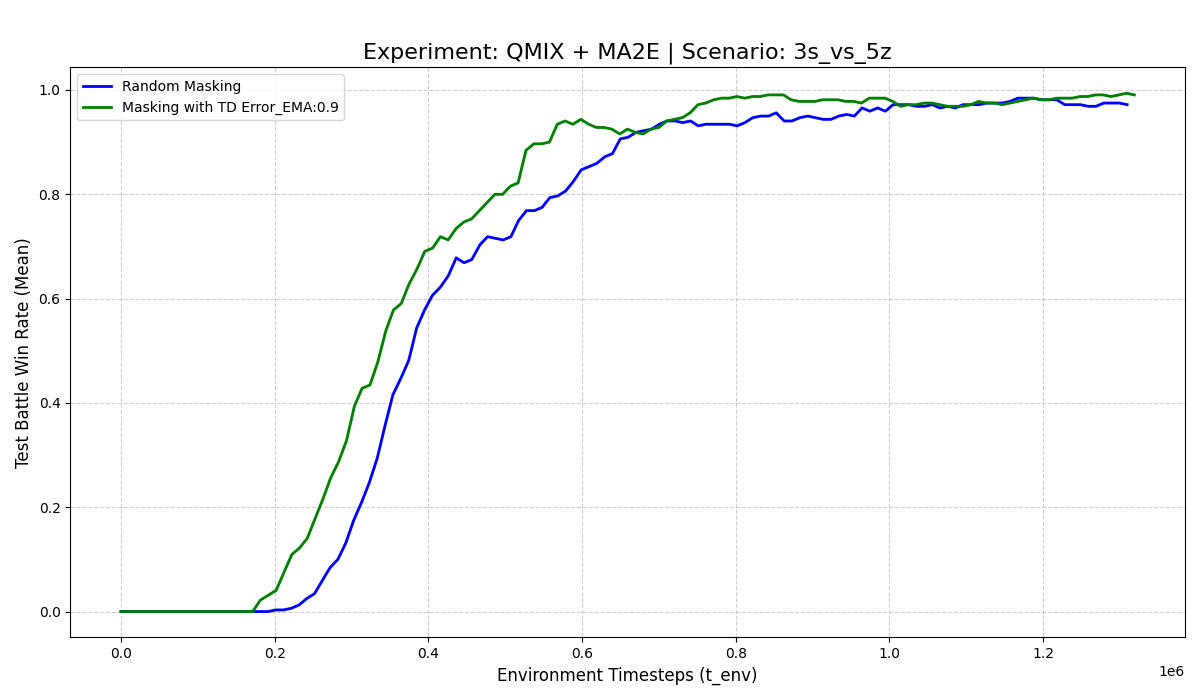
\includegraphics[width=0.5\textwidth]{images_pfe/results_li-ma2e/test_battle_won_mean_3s_vs_5z_ema_0.9_smoothed.png}}%
\hfill%
\subfloat[\label{fig:ema_0.1} EMA with ($\alpha=0.1$)]{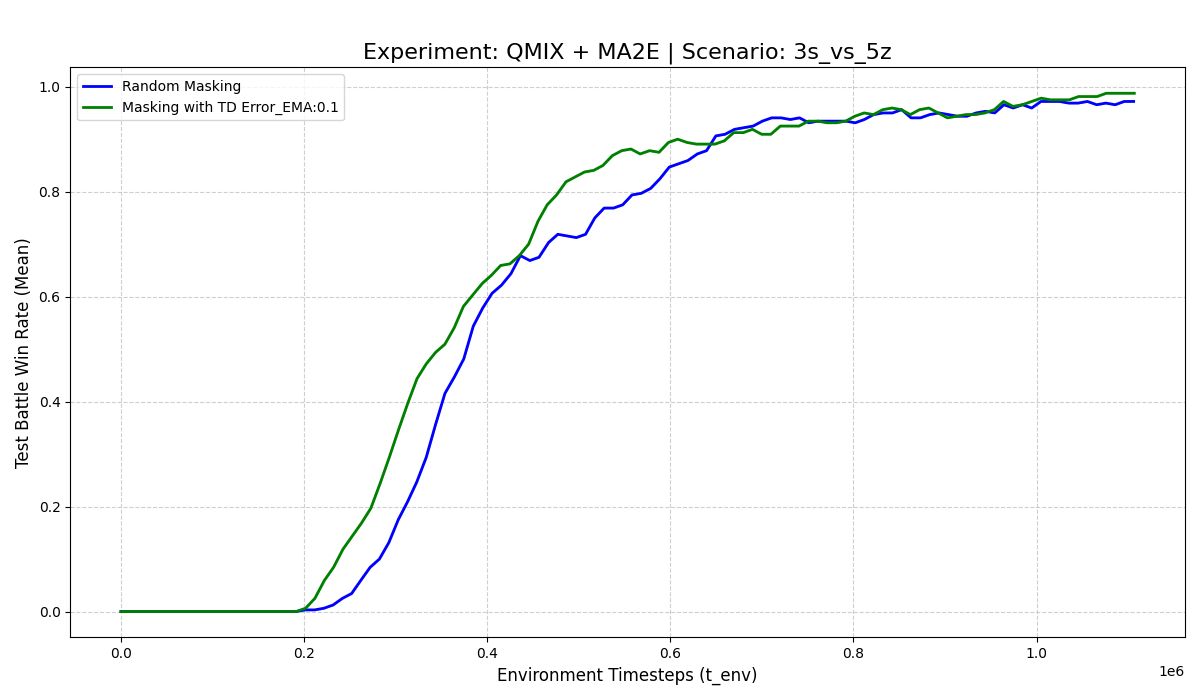
\includegraphics[width=0.5\textwidth]{images_pfe/results_li-ma2e/test_battle_won_mean_3s_vs_5z_ema_0.1_smoothed.png}}%
\caption{Performance comparison of EMA-based masking strategies with different decay rates $\alpha$ against the baseline Random Masking on the \texttt{3s\_vs\_5z} SMAC map. The plots show the mean test win rate over environment timesteps.}
\label{fig:ema_comparison}
\end{figure}
The performance of the EMA strategy with a decay rate of $\alpha=0.9$ was compared against the baseline Random Masking, with the results for the \texttt{3s\_vs\_5z} scenario presented in Figure~\ref{fig:ema_comparison}.
The results clearly demonstrate that our EMA-based masking (green line) achieves significantly better sample efficiency than the baseline (blue line). The $LI-{MA}^2E$ framework learns the task much faster, reaching a high win rate at approximately 0.6 million timesteps, while the baseline requires around 0.8 million timesteps to achieve similar performance. While both methods eventually converge to a near-perfect win rate on this map, the accelerated learning curve of the EMA method confirms our hypothesis that intelligently guiding the masking process is more effective than a random strategy.

Despite this improved efficiency, the limitation of this global EMA approach is its inherent inertia. An agent that has recently improved its policy might still be masked due to its poor history, potentially slowing down optimal convergence. This observation motivated the development of our next method, which analyzes performance dynamics on a more granular, intra-episode level.


\subsection{Method 2: Variance-Directional-Drop Score (VDS)}
\label{subsec:vds_method}

Our second approach analyzes the dynamics of an agent's TD-error within a single episode. The VDS was designed to identify which agents are \textit{learning}, which are \textit{forgetting}, and how turbulent their learning process is. The hypothesis is that the best candidates for masking are agents whose performance is not only getting worse but is also highly unstable.

\paragraph{Implementation Details}
The VDS score is a product of two factors: a Variance Factor that measures turbulence and a Directional-Drop Factor that measures the learning trend. The formula is defined as:
\begin{equation}
    \text{VDS} = \left(\frac{\sigma^2}{\sigma^2 + 1}\right) \times \left(\frac{e_0 - e_T}{|e_0| + \epsilon}\right)
\label{eq:vds}
\end{equation}

\begin{itemize}
\item \textbf{$\left(\frac{\sigma^2}{\sigma^2 + 1}\right)$ : } This term quantifies the \textit{turbulence} or volatility of an agent's TD-error curve throughout the episode. A value close to 1 signifies a \textit{bumpy} learning process with significant oscillations and spikes, while a value close to 0 indicates a smooth and calm learning curve. This factor rewards episodes that are eventful.
\item \textbf{$\left(\frac{e_0 - e_T}{|e_0| + \epsilon}\right)$} This term determines the overall trend of the error from the start of the episode. A positive result signifies that the agent is \textit{learning}, as its prediction error has dropped. Conversely, a negative result signifies that the agent is \textit{forgetting,} as its error has increased over the course of the episode.
\end{itemize}

By multiplying these factors, the sign of the resulting VDS score indicates whether an agent is a learner (+) or a forgetter (−), while the magnitude reflects the drama of the change. Our masking strategy prioritizes agents identified as \textit{chaotic forgetters}: those who exhibit both high variance and a negative directional drop. These agents yield a large negative VDS score and are masked first, forcing the MAE to focus its representational power on the most unstable and deteriorating policies.

\paragraph{Results and Limitations}

\begin{figure}[h]
    \centering
    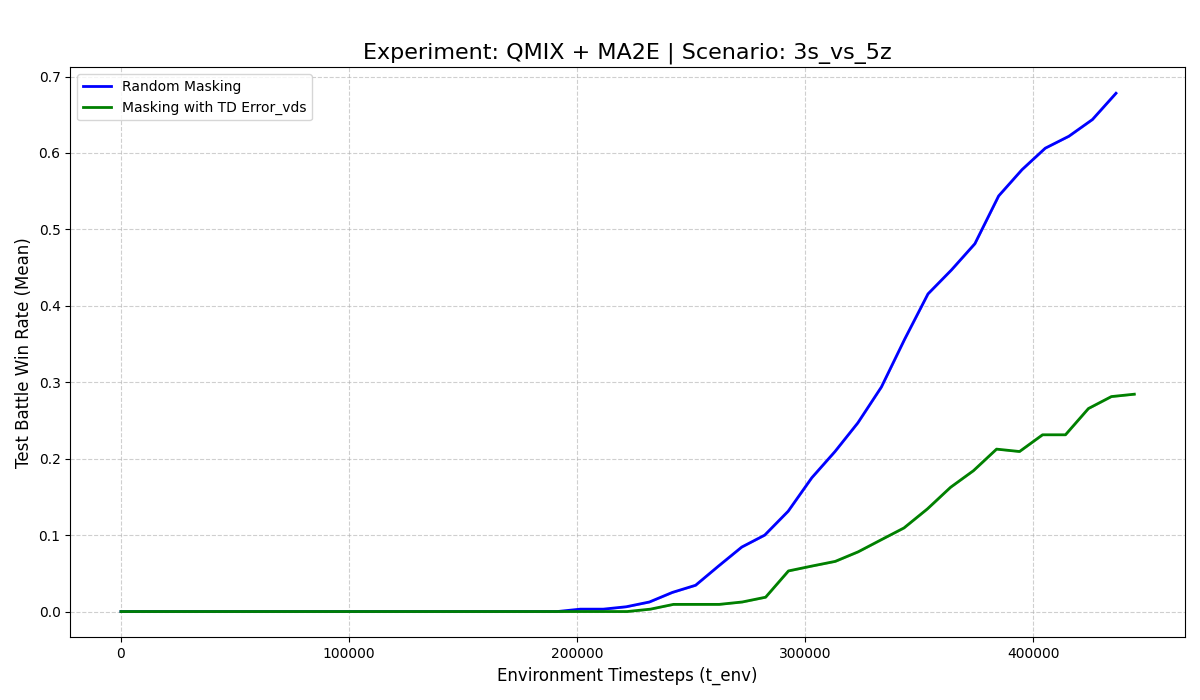
\includegraphics[width=0.8\textwidth]{images_pfe/results_li-ma2e/test_battle_won_mean_3s_vs_5z_vds_smoothed.png}
    \caption{Performance comparison of the VDS masking strategy against the baseline Random Masking on the \texttt{3s\_vs\_5z} SMAC map. The plot shows the mean test win rate over environment timesteps.}
    \label{fig:vds_vs_random}
\end{figure}

The performance of the VDS masking strategy was compared against the baseline Random Masking, with the results for the \texttt{3s\_vs\_5z} scenario presented in Figure~\ref{fig:vds_vs_random}.

Contrary to our initial hypothesis, the results show that the VDS masking strategy (green line) significantly underperforms compared to the baseline Random Masking (blue line). Throughout the training process, the win rate for the VDS-guided agent remains considerably lower than that of the agent using a random strategy. By the end of the depicted training run at approximately 450,000 timesteps, the baseline achieves a win rate of nearly 70\%, while the VDS method struggles to surpass 30\%.

Given the clear negative performance trend and the computational time required, the experiment for the VDS method was halted early, as it was evident that further training was unlikely to yield a competitive result.

This poor performance likely stems from the core limitations of the VDS metric. By relying on the start and end points of an entire episode, VDS may generate a noisy or misleading signal. For instance, an episode with high variance in the TD-error could result in a high-magnitude VDS score, causing a potentially effective agent to be masked frequently. As discussed, the directional-drop component also fails to distinguish between an agent that is truly \textit{forgetting } and one that is simply encountering a difficult, new part of the state space. The combination of these factors appears to create a disruptive, rather than helpful, curriculum for the MAE module, ultimately hindering the overall learning process. This result underscores the difficulty of designing a robust masking heuristic and strongly motivates the development of a more reliable score, REFDS, which focuses on recent-step dynamics.
A key limitation of \texttt{VDS} lies in its interpretation of an increasing TD-error trend as definitive \textit{forgetting}. While an agent's error increasing over an episode can be a signal of forgetting, this is not always the case. The rising TD-error could mean one of two distinct things:

\begin{enumerate}
    \item \textbf{Forgetting or Poor Generalization:} If an agent has seen the early parts of an episode's trajectory more often during training, it will predict those values well, leading to a low TD-error. If the error then rises in the later, less-frequently seen states, it suggests the agent may have \textit{forgotten} how to behave there or has failed to generalize its knowledge from the familiar states. This is a plausible sign of forgetting.
    
    \item \textbf{Encountering Under-Trained States:} If the later states in the trajectory are simply underrepresented in the replay buffer, a high TD-error is not a sign of forgetting, but rather an indication that the agent is still actively learning about this unfamiliar part of the state space.
\end{enumerate}
However, its reliance on the start and end points of an entire episode can sometimes be misleading. For example, an agent might improve significantly for most of the episode but then start to \textit{forget} right at the end; VDS might still classify this as overall \textit{learning} and fail to mask the agent when it needs it most. This limitation motivated the development of a score that focuses specifically on the most recent timesteps.


\subsection{Method 3: Recent Error and Forgetting Detection (REFDS)}
\label{subsec:REFDS_method}

To overcome the full-episode focus of VDS and its inability to capture short-term dynamics, we developed REFDS. This score is designed to identify agents that are problematic \textit{right now} by analyzing only the most recent timesteps of their experience. The hypothesis is that a more accurate and timely signal can be derived by considering two factors from an agent's recent history: its current average error level and any immediate evidence of \textit{forgetting} (a rising error trend).


\paragraph{Implementation Details}

The \texttt{REFDS} score is computed per-agent using only the most recent batch of TD-errors, focusing on the last 25\% of each trajectory \\ ($k = \lfloor \text{trajectory\_length} / 4 \rfloor$) to capture recent performance trends. It combines the mean TD-error (magnitude of recent errors) and the slope of TD-errors (directional trend, penalizing worsening performance).
The score is calculated as:
\begin{equation}
    \text{REFDS} = 0.6 \cdot \overline{|\text{TD}|}_k + 0.4 \cdot \text{ReLU}(\text{slope}_k)
    \label{eq:REFDS}
\end{equation}

where $\overline{|\text{TD}|}_k$ is the mean of absolute TD-errors over the last $k$ steps, and $\text{slope}_k$ is the trend over that same window.

\paragraph{Key Properties}
\begin{itemize}
    \item \textbf{Timestep-Local:} Uses only the latest batch of experience, requiring no historical data buffer.
    \item \textbf{Adaptive:} The score naturally targets agents with either large-magnitude errors or a worsening error trend, focusing learning where it is most needed.
\end{itemize}


This approach ensures that fine-tuning prioritizes agents with immediate, high-impact errors while remaining computationally lightweight. The weights (0.6, 0.4) and the window size $k$ are tunable hyperparameters that balance the sensitivity between error magnitude and trend severity.



\paragraph{The purpose of the ReLU function in the REFDS Formula: }
The purpose of the ReLU function is to isolate and penalize only the agents that are actively \textit{forgetting}, without penalizing agents that are actively learning.
Here's the breakdown of the logic:
\begin{itemize}
    \item \textbf{The $\text{slope}_k$ term, $(\text{TD}_{\text{end}} – \text{TD}_{\text{mid}}) / k$}, calculates the recent trend of the TD-error.
   \item By applying $\text{ReLU}(\text{slope}_k)$, we transform the slope value:
\begin{itemize}
    \item If the slope is positive (forgetting), ReLU passes the value through, adding a penalty to the \texttt{REFDS} score.
    \item If the slope is negative (learning), ReLU outputs zero. This is crucial because it ensures that agents who are learning effectively are not \textit{penalized twice} for having a steep (but beneficial) drop in their error.
\end{itemize}
    % \item A positive slope indicates that the error is increasing, which is our signal for \textit{forgetting}.
    % \item A negative slope indicates that the error is decreasing, which is a sign of successful learning.
\end{itemize}
% By applying $\text{ReLU}(\text{slope}_k)$, we transform the slope value:
% \begin{itemize}
%     \item If the slope is positive (forgetting), ReLU passes the value through, adding a penalty to the \texttt{REFDS} score.
%     \item If the slope is negative (learning), ReLU outputs zero. This is crucial because it ensures that agents who are learning effectively are not \textit{penalized twice} for having a steep (but beneficial) drop in their error.
% \end{itemize}
The ReLU acts as a filter, allowing the formula to focus exclusively on the undesirable behavior of an upward drift in error, making the \textit{Forget-Penalty} term more precise.
\paragraph{Results and Limitations}
\begin{figure}[h]
    \centering
   
        
    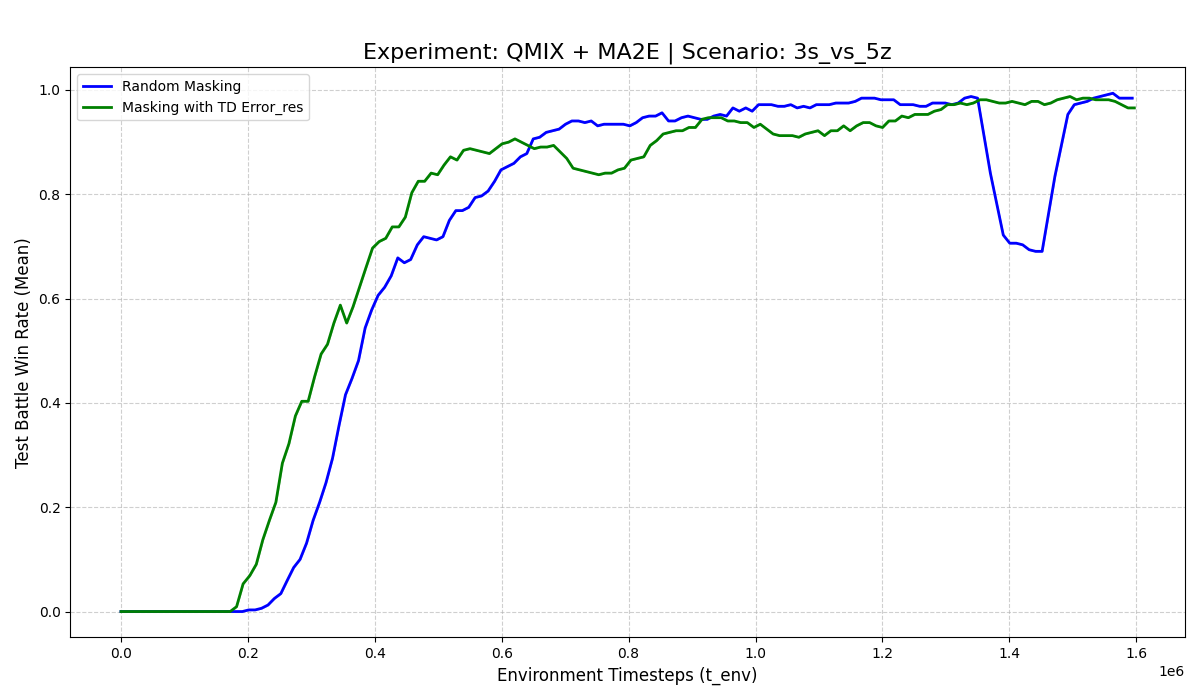
\includegraphics[width= 0.9\linewidth]{images_pfe/results_li-ma2e/test_battle_won_mean_3s_vs_5z_res_smoothed_full.png}
 
  
    \caption{Performance comparison of the REFDS masking strategy against the baseline Random Masking on the \texttt{3s\_vs\_5z} SMAC map. The plot shows the mean test win rate over environment timesteps.
    }
    \label{fig:REFDS_vs_random}
\end{figure}

The performance of the REFDS masking strategy was compared against the baseline Random Masking on the \texttt{3s\_vs\_5z} scenario, with the results presented in Figure~\ref{fig: REFDS_vs_random}.

The results clearly demonstrate that the REFDS strategy (green line) provides a significant improvement in sample efficiency over the baseline (blue line). The REFDS method begins learning notably earlier and maintains a consistent performance lead throughout the critical training phase between approximately 0.2 million and 0.8 million timesteps.

While the Random Masking baseline eventually catches up and both methods are capable of solving this map by reaching a near-perfect win rate, the accelerated learning curve of REFDS is substantial. This confirms that a focused masking strategy based on recent learning dynamics is highly effective at speeding up the training process compared to an uninformed, random approach.

\texttt{REFDS} introduces its own set of challenges and limitations:
\begin{itemize}
    \item \textbf{Computational Overhead:} Compared to the simpler EMA or VDS scores, calculating \texttt{REFDS} for every agent at every episode is more computationally intensive, as it requires storing and processing a sliding window of recent TD-errors.
    
    \item \textbf{Hyperparameter Sensitivity:} The performance of \texttt{REFDS} is dependent on the careful tuning of its key hyperparameters.
    \begin{itemize}
        \item \textit{Window Size ($k$):} The choice of the look-back window is a trade-off. A shorter window reacts faster but can be noisy, while a longer window is smoother but slower to adapt. The optimal value can be scenario-dependent.
        
        \item \textit{Component Weights (0.6 / 0.4):} The weights assigned to the mean-error versus the forgetting-penalty must be balanced. Over-emphasizing one component can cause the score to miss the nuances of the other, requiring careful adjustment to achieve the best results.
    \end{itemize}
\end{itemize}
However, REFDS still operates on the TD-error in isolation. It treats all errors equally, regardless of the context provided by an agent's observation. For example, a high TD-error from an agent seeing very little might be less informative for the MAE to reconstruct than a high TD-error from an agent observing a complex battlefield interaction. This realization prompted our final investigation into a method that contextualizes the error signal with the agent's observation.
\subsection{Method 4: Observation-Weighted TD-Error}

Our final investigation attempted to contextualize an agent's learning error with the \textit{richness} of its observation. The previous methods, including REFDS, treat the TD-error signal in isolation. However, a high TD-error from an agent seeing very little might be less informative for the MAE to reconstruct than a high TD-error from an agent observing a complex battlefield interaction.
The hypothesis for this method is that an agent's failure is most significant if it is failing despite receiving a large amount of information. To quantify the amount of information an agent is \textit{seeing,} we use the L2 norm of its observation vector.

\paragraph{Implementation Details}
The masking score is calculated as a direct product of the agent's performance error and its observation magnitude:
\begin{equation}
    \text{Masking Score} = |\text{TD-error}| \times \| \text{Observation} \|_2
    \label{eq:obs_weighted_td}
\end{equation}
The intuition behind this score can be broken down into four cases:
\begin{itemize}
    \item \textbf{High TD-error \& High L2-norm:} The agent receives a lot of information but still fails to predict correctly. It is likely \textit{confused} or \textit{overwhelmed} and is a prime candidate for masking.
    \item \textbf{High TD-error \& Low L2-norm:} The agent sees very little and is still performing poorly. Its observation is uninformative, making it another good candidate for masking.
    \item \textbf{Low TD-error \& High L2-norm:} The agent sees a lot and learns well. This is a strong, stable agent that should be kept as an anchor for the MAE's reconstruction.
    \item \textbf{Low TD-error \& Low L2-norm:} The agent is stable but has a limited view. This agent is likely harmless and can be kept.
\end{itemize}

\paragraph{Results and Limitations}


\begin{figure}[h]
    \centering
    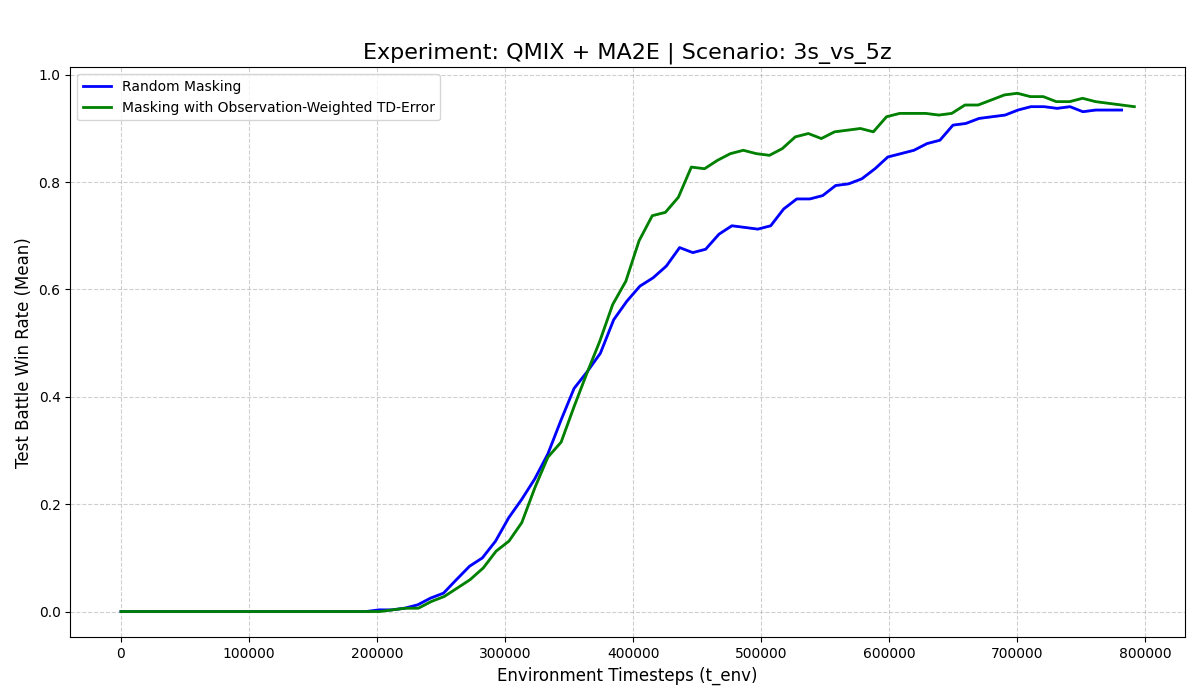
\includegraphics[width=0.8\textwidth]{images_pfe/results_li-ma2e/test_battle_won_mean_3s_vs_5z_Observation-Weighted_TD_smoothed.png}
    \caption{Performance comparison of the Observation-Weighted TD-Error masking strategy against the baseline Random Masking on the \texttt{3s\_vs\_5z} SMAC map. The plot shows the mean test win rate over environment timesteps.}
    \label{fig:obs_weighted_vs_random}
\end{figure}

The performance of the Observation-Weighted TD-Error strategy was compared against the Random Masking baseline on the \texttt{3s\_vs\_5z} map, with results shown in Figure~\ref{fig:obs_weighted_vs_random}.

The results present a nuanced picture. Unlike some previously tested methods, this strategy does not show a significant improvement in sample efficiency during the initial learning phase. The performance of the observation-weighted method (green line) closely tracks that of the random baseline (blue line) for the first approximately 450,000 timesteps.

However, in the later stages of training, a clear advantage emerges. The Observation-Weighted TD-Error strategy begins to outperform the baseline, converging to a high win rate more quickly and smoothly. This delayed improvement supports our analysis of the method's limitations; the L2 norm of the observation is not always a reliable or stable proxy for the usefulness of the information an agent receives. The initial phase, where it performs similarly to random masking, suggests that this heuristic may introduce noise that counteracts the benefit of the TD-error signal early in training. Only once the underlying value functions become more stable does the contextual information from the observation norm appear to provide a consistent, beneficial signal.

\subsection{Method 5: Adaptive Masking with Mean TD-Error Thresholding}

After investigating complex heuristics like VDS and observation-weighting, our final approach returns to the most direct signal of agent performance: the TD-error itself. The previous methods, while insightful, introduced additional complexity and sensitive hyperparameters. The hypothesis for this final method is that a simple, direct, and adaptive threshold is more robust and effective.

Instead of trying to interpret the dynamics of the error (like VDS or REFDS), we simply posit that agents performing worse than the current batch average are the most beneficial candidates for masking. This approach is designed to be adaptive throughout training. Early on, when agent performance varies widely, the mean TD-error provides a natural and dynamic cutoff. Late in training, when all agents perform well and have similar, low TD errors, a fixed threshold would fail. Therefore, a top-$k_1$ fallback mechanism is included to ensure that the MAE continues to be fine-tuned on the relatively weaker agents, even when all agents are strong.

\paragraph{Implementation Details}
It is important to note that this smart masking strategy is only applied during the policy fine-tuning phase. The initial pre-training of the MA$^2$E module is still conducted using random masking to allow the model to learn general, unbiased agent representations.

The fine-tuning process for this method uses only the TD errors generated from the most recent training batch, ensuring minimal overhead. The step-by-step process is as follows:
\begin{enumerate}
    \item \textbf{Compute TD-Error per Agent:} For each agent $a$, the TD-error is calculated as the difference between its predicted Q-value and the target value:
    \begin{equation}
        \label{eq:td_error_simple}
        \text{TD-error}_a = Q_a - \text{Target}_a
    \end{equation}

    \item \textbf{Agent Selection with Adaptive Threshold:} The core of the method lies in its two-stage selection logic:
    \begin{itemize}
        \item First, the mean of the absolute TD-errors is computed across all agents in the current training batch.
        \item Any agent whose individual TD-error is above this batch mean is selected for masking.
        \item As a fallback, if no agent's error exceeds the mean (a situation common late in training), the top-$k$ agents with the highest TD-errors are chosen instead.
    \end{itemize}

    \item \textbf{Apply Masking:} The observation-action history tokens of all selected agents are masked (e.g., zeroed out) before being passed as input to the MAE module for reconstruction.
\end{enumerate}
\paragraph{Results and Limitations}

\begin{figure}[h]
    \centering
    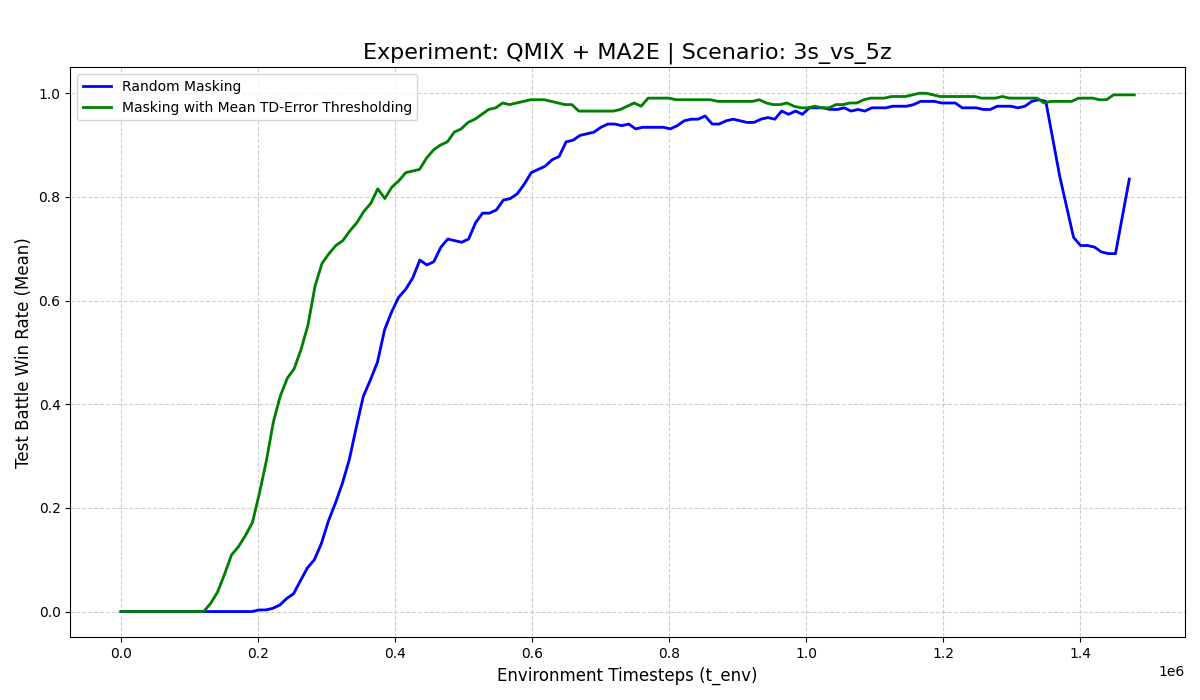
\includegraphics[width=0.8\textwidth]{images_pfe/results_li-ma2e/test_battle_won_mean_3s_vs_5z_Mean_TD-Error_Thresholding _smoothed.png}
    \caption{Performance of the final Adaptive Mean TD-Error Thresholding strategy compared against the Random Masking baseline on the \texttt{3s\_vs\_5z} SMAC map. The plot highlights the superior sample efficiency of the proposed method.}
    \label{fig:mean_td_vs_random}
\end{figure}


Finally, the performance of our proposed Adaptive Masking with Mean TD-Error Thresholding was compared against the baseline Random Masking. The results on the \texttt{3s\_vs\_5z} map are presented in Figure~\ref{fig:mean_td_vs_random}.

The results demonstrate a dramatic improvement in performance and sample efficiency. The Mean TD-Error Thresholding strategy (green line) learns significantly faster than the baseline (blue line), achieving a near-perfect win rate before 0.6 million timesteps, while the baseline requires over 1.2 million timesteps to reach a similar level of performance.

This final experiment provides a clear conclusion to our investigation of scoring methods. After exploring a global historical average (EMA), episode-level dynamics (VDS), and feature-based heuristics (Observation-Weighted TD-error), the results show that a simple, direct, and adaptive threshold based on the batch-average TD-error is the most robust and effective strategy. It avoids the inertia of the EMA, the ambiguity of VDS, and the heuristic instability of the observation-weighted score. Its superior performance validates our final hypothesis that a straightforward comparison of an agent's immediate error to that of its peers provides the cleanest and most potent signal for guiding the MAE's representational learning.

Therefore, based on this comprehensive empirical analysis, the Adaptive Masking with \textbf{Mean TD-Error Thresholding} was selected as the definitive $LI-{MA}^2E$ framework. All subsequent results presented in this thesis will utilize this final, optimized method.
% This new subsection will contain the summary plot and its analysis.
\subsection{Comparison of Masking Strategies:}

To synthesize the findings from our investigation and provide a clear visual summary, Figure~\ref{fig:all_strategies_comparison} presents a direct comparison of all tested masking strategies on the  \texttt{3s\_vs\_5z} scenario.
\begin{figure}[h]
    \centering
    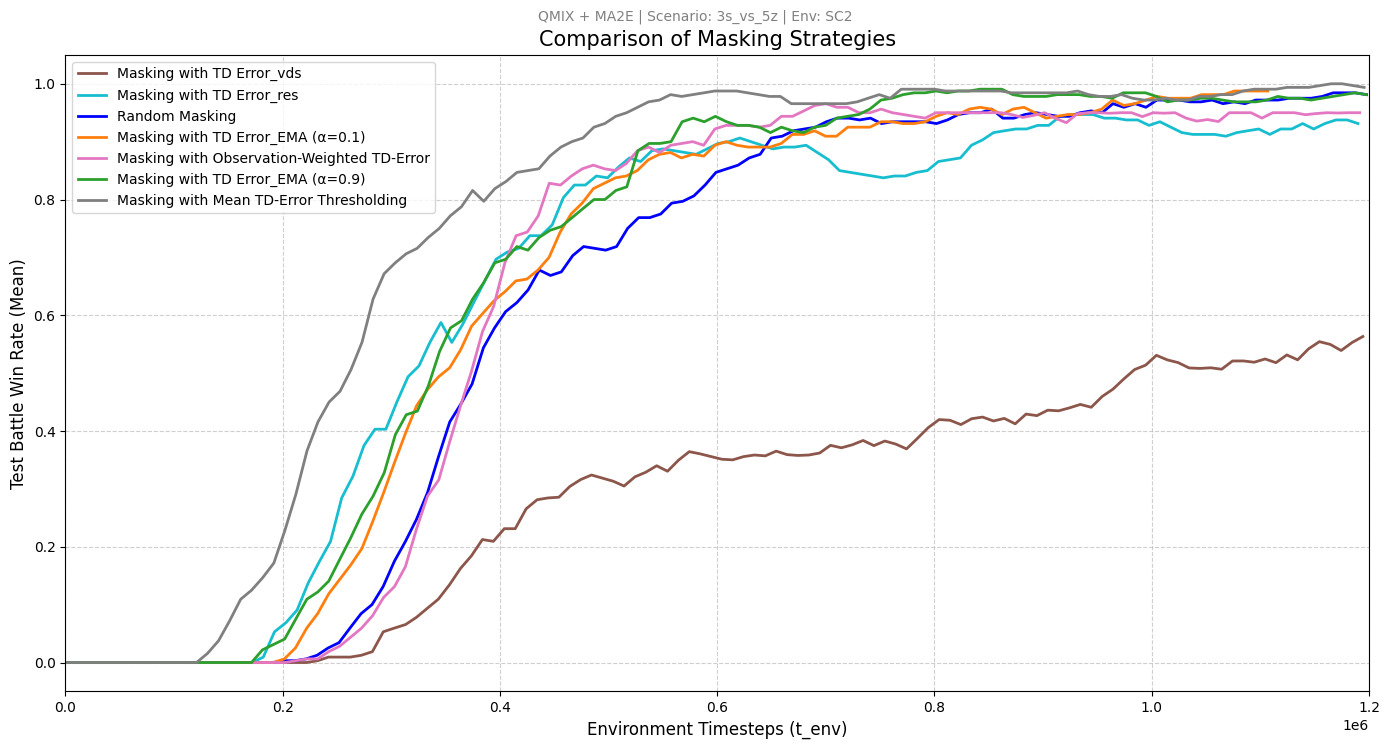
\includegraphics[width=1.0\textwidth]{images_pfe/results_li-ma2e/compare_scores.jpg} 
    \caption{Comprehensive comparison of all evaluated masking strategies on the \texttt{3s\_vs\_5z}  SMAC map. The results visually confirm that the Mean TD-Error Thresholding and REFDS strategies provide the best sample efficiency.}
    \label{fig:all_strategies_comparison}
\end{figure}

The results in Figure~\ref{fig:all_strategies_comparison} provide a clear hierarchy of performance. The \textbf{VDS} strategy significantly hindered learning compared to the random baseline. The \textbf{EMA-based methods} and the \textbf{Observation-Weighted TD-Error} offer marginal improvements over random masking, with the more reactive \textbf{EMA($\alpha=0.9$)} showing the most promise among them.

However, the two most effective strategies are clearly \textbf{REFDS} and our final proposed method, \textbf{Mean TD-Error Thresholding}. Both demonstrate vastly superior sample efficiency, reaching high win rates much earlier than any other approach. This comprehensive result validates our research trajectory, confirming that moving from global averages or flawed episode-level heuristics to reactive, fine-grained signals based on recent TD-error dynamics yields the best performance. While both REFDS and Mean TD-Error Thresholding are highly effective, the latter was chosen as our final framework due to its simpler implementation and more direct, adaptive logic.

% \section{Main Results: Comparative Performance of LI-MA2E}
% \label{sec:main_results}

% Having established the superiority of our Adaptive Mean TD-Error Thresholding strategy in the previous section, we now present a comprehensive performance evaluation of the final LI-MA2E framework. To validate its effectiveness and generalization capabilities, we benchmark our method against the baseline MA2E with random masking across a suite of challenging HARD, MEDIUM, and easy scenarios from the SMAC environment. This section will demonstrate the consistent performance gains achieved by our intelligent masking approach.
% \subsection{Performance on SMAC Scenarios}


% \subsubsection{Scenario: \texttt{3m}}
% Our first evaluation is on the \texttt{3m} scenario, a simple symmetric map that pits \textbf{3 allied Marines against 3 enemy Marines}. Because  \textbf{the agents are homogeneous} and the \textbf{setup is symmetric}, the primary challenge in this map is learning a fundamental cooperative tactic: \textbf{focus-firing}. To win consistently, all three agents must learn to coordinate their attacks on the same enemy target at the same time to eliminate it quickly, rather than spreading their damage ineffectually across multiple targets. This scenario serves as a basic test of coordination. The results are presented in Figure~\ref{fig:3m}.

% \begin{figure}[h]
%     \centering
%     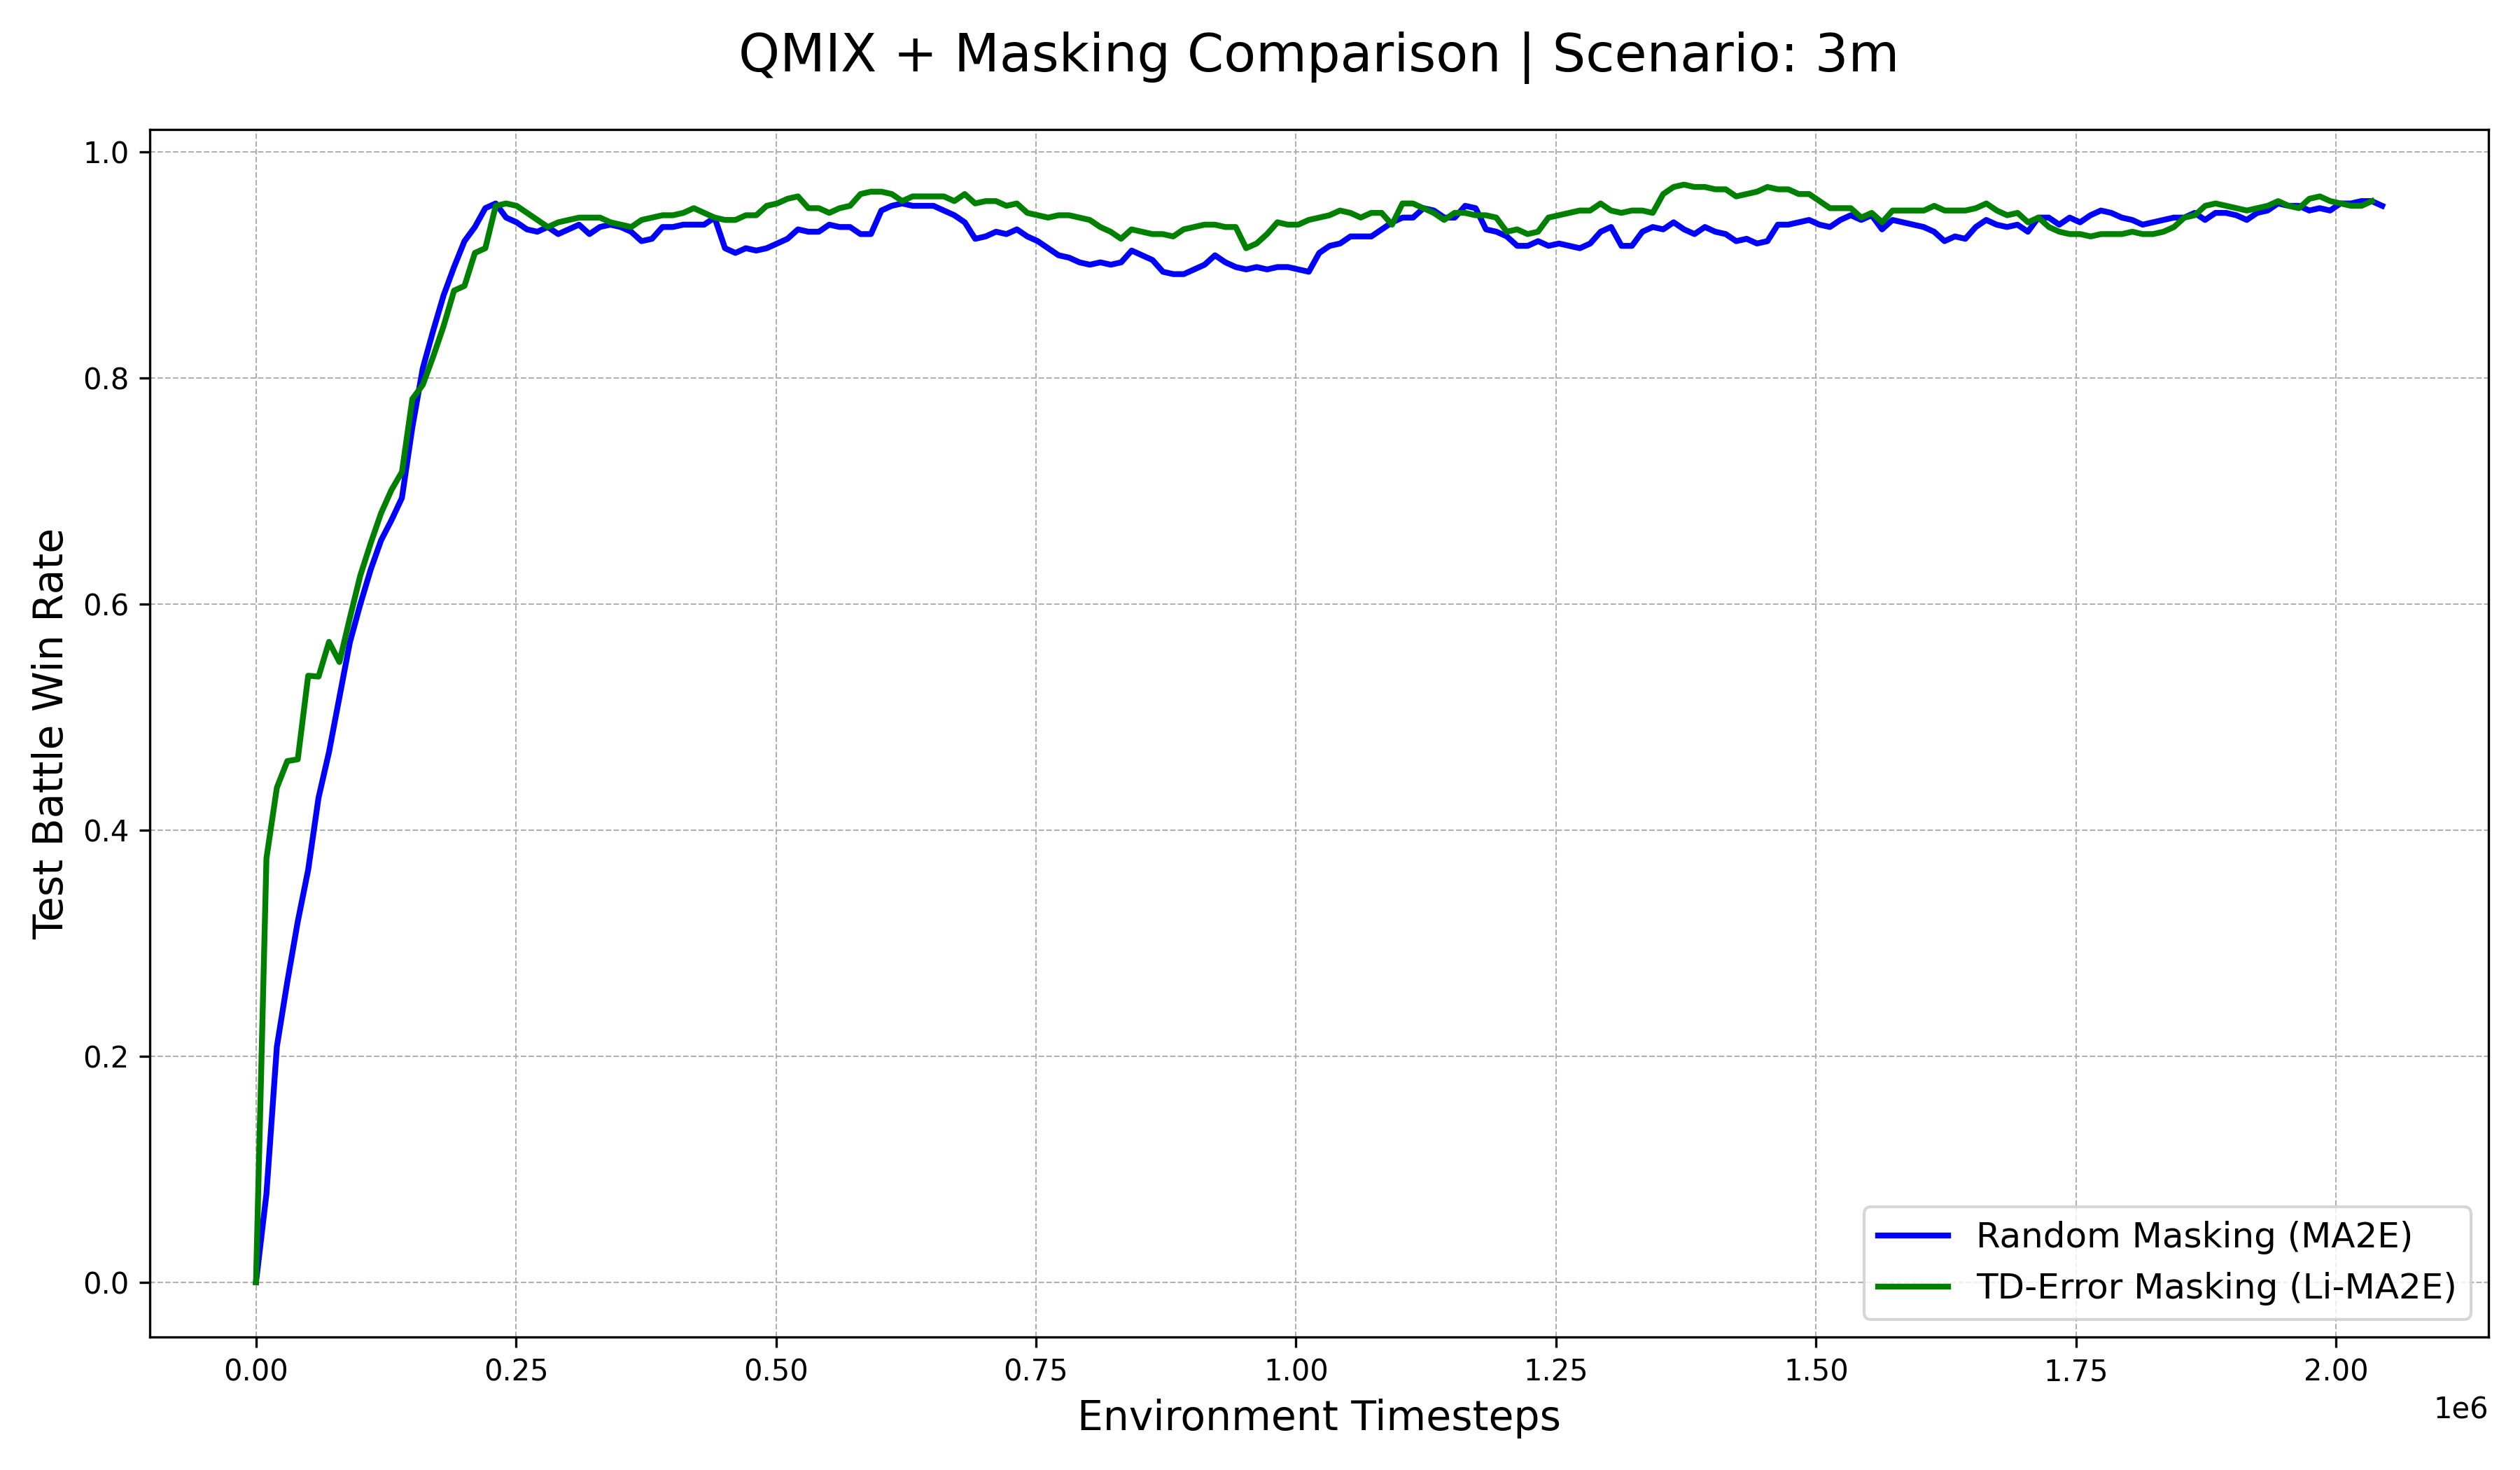
\includegraphics[width=0.8\textwidth]{images_pfe/results_li-ma2e/comparison_plot_3m.png}
%     \caption{Performance comparison on the \texttt{3m} SMAC map. In this simple symmetric scenario, the performance of LI-MA2E is comparable to the random masking baseline.}
%     \label{fig:3m}
% \end{figure}

% \paragraph{Analysis}
% As the learning curves in Figure~\ref{fig:3m} show, the performance of our LI-MA2E framework (green line) is largely comparable to that of the baseline MA2E with random masking (blue line). Both methods learn the task very rapidly, achieving a near-perfect win rate in under 250,000 environment timesteps. Throughout the remainder of the training, both policies maintain a similar high level of performance.

% This result suggests that in simpler scenarios where the need for complex coordination to overcome partial observability is low, the additional guidance provided by our intelligent masking strategy does not yield a significant advantage. The baseline random masking is sufficient for the MAE module to learn the necessary representations to solve this task effectively. This provides an important baseline, demonstrating that our method's complexity does not hinder performance on easy tasks while setting the stage for evaluation on more demanding scenarios.

% \subsubsection{Scenario: \texttt{3s\_vs\_3z}}
% Next, we look at the \texttt{3s\_vs\_3z} scenario. In this test, our \textbf{3 agents control Stalker units}, which can attack from a distance. They face \textbf{3 enemy Zealot units}, which are severe but can only attack up close.

% Because our agents can shoot from far away, the most important skill they must learn is called \textbf{kiting}. Kiting means the Stalkers must keep moving away from the chasing Zealots, while stopping briefly to shoot at them. The goal is to damage the enemy without letting them get close enough to hit back. To do this well, all three of our agents need to work together as a team. The results of this test are shown in Figure~\ref{fig:3s_vs_3z}.

% \begin{figure}[h]
%     \centering
%     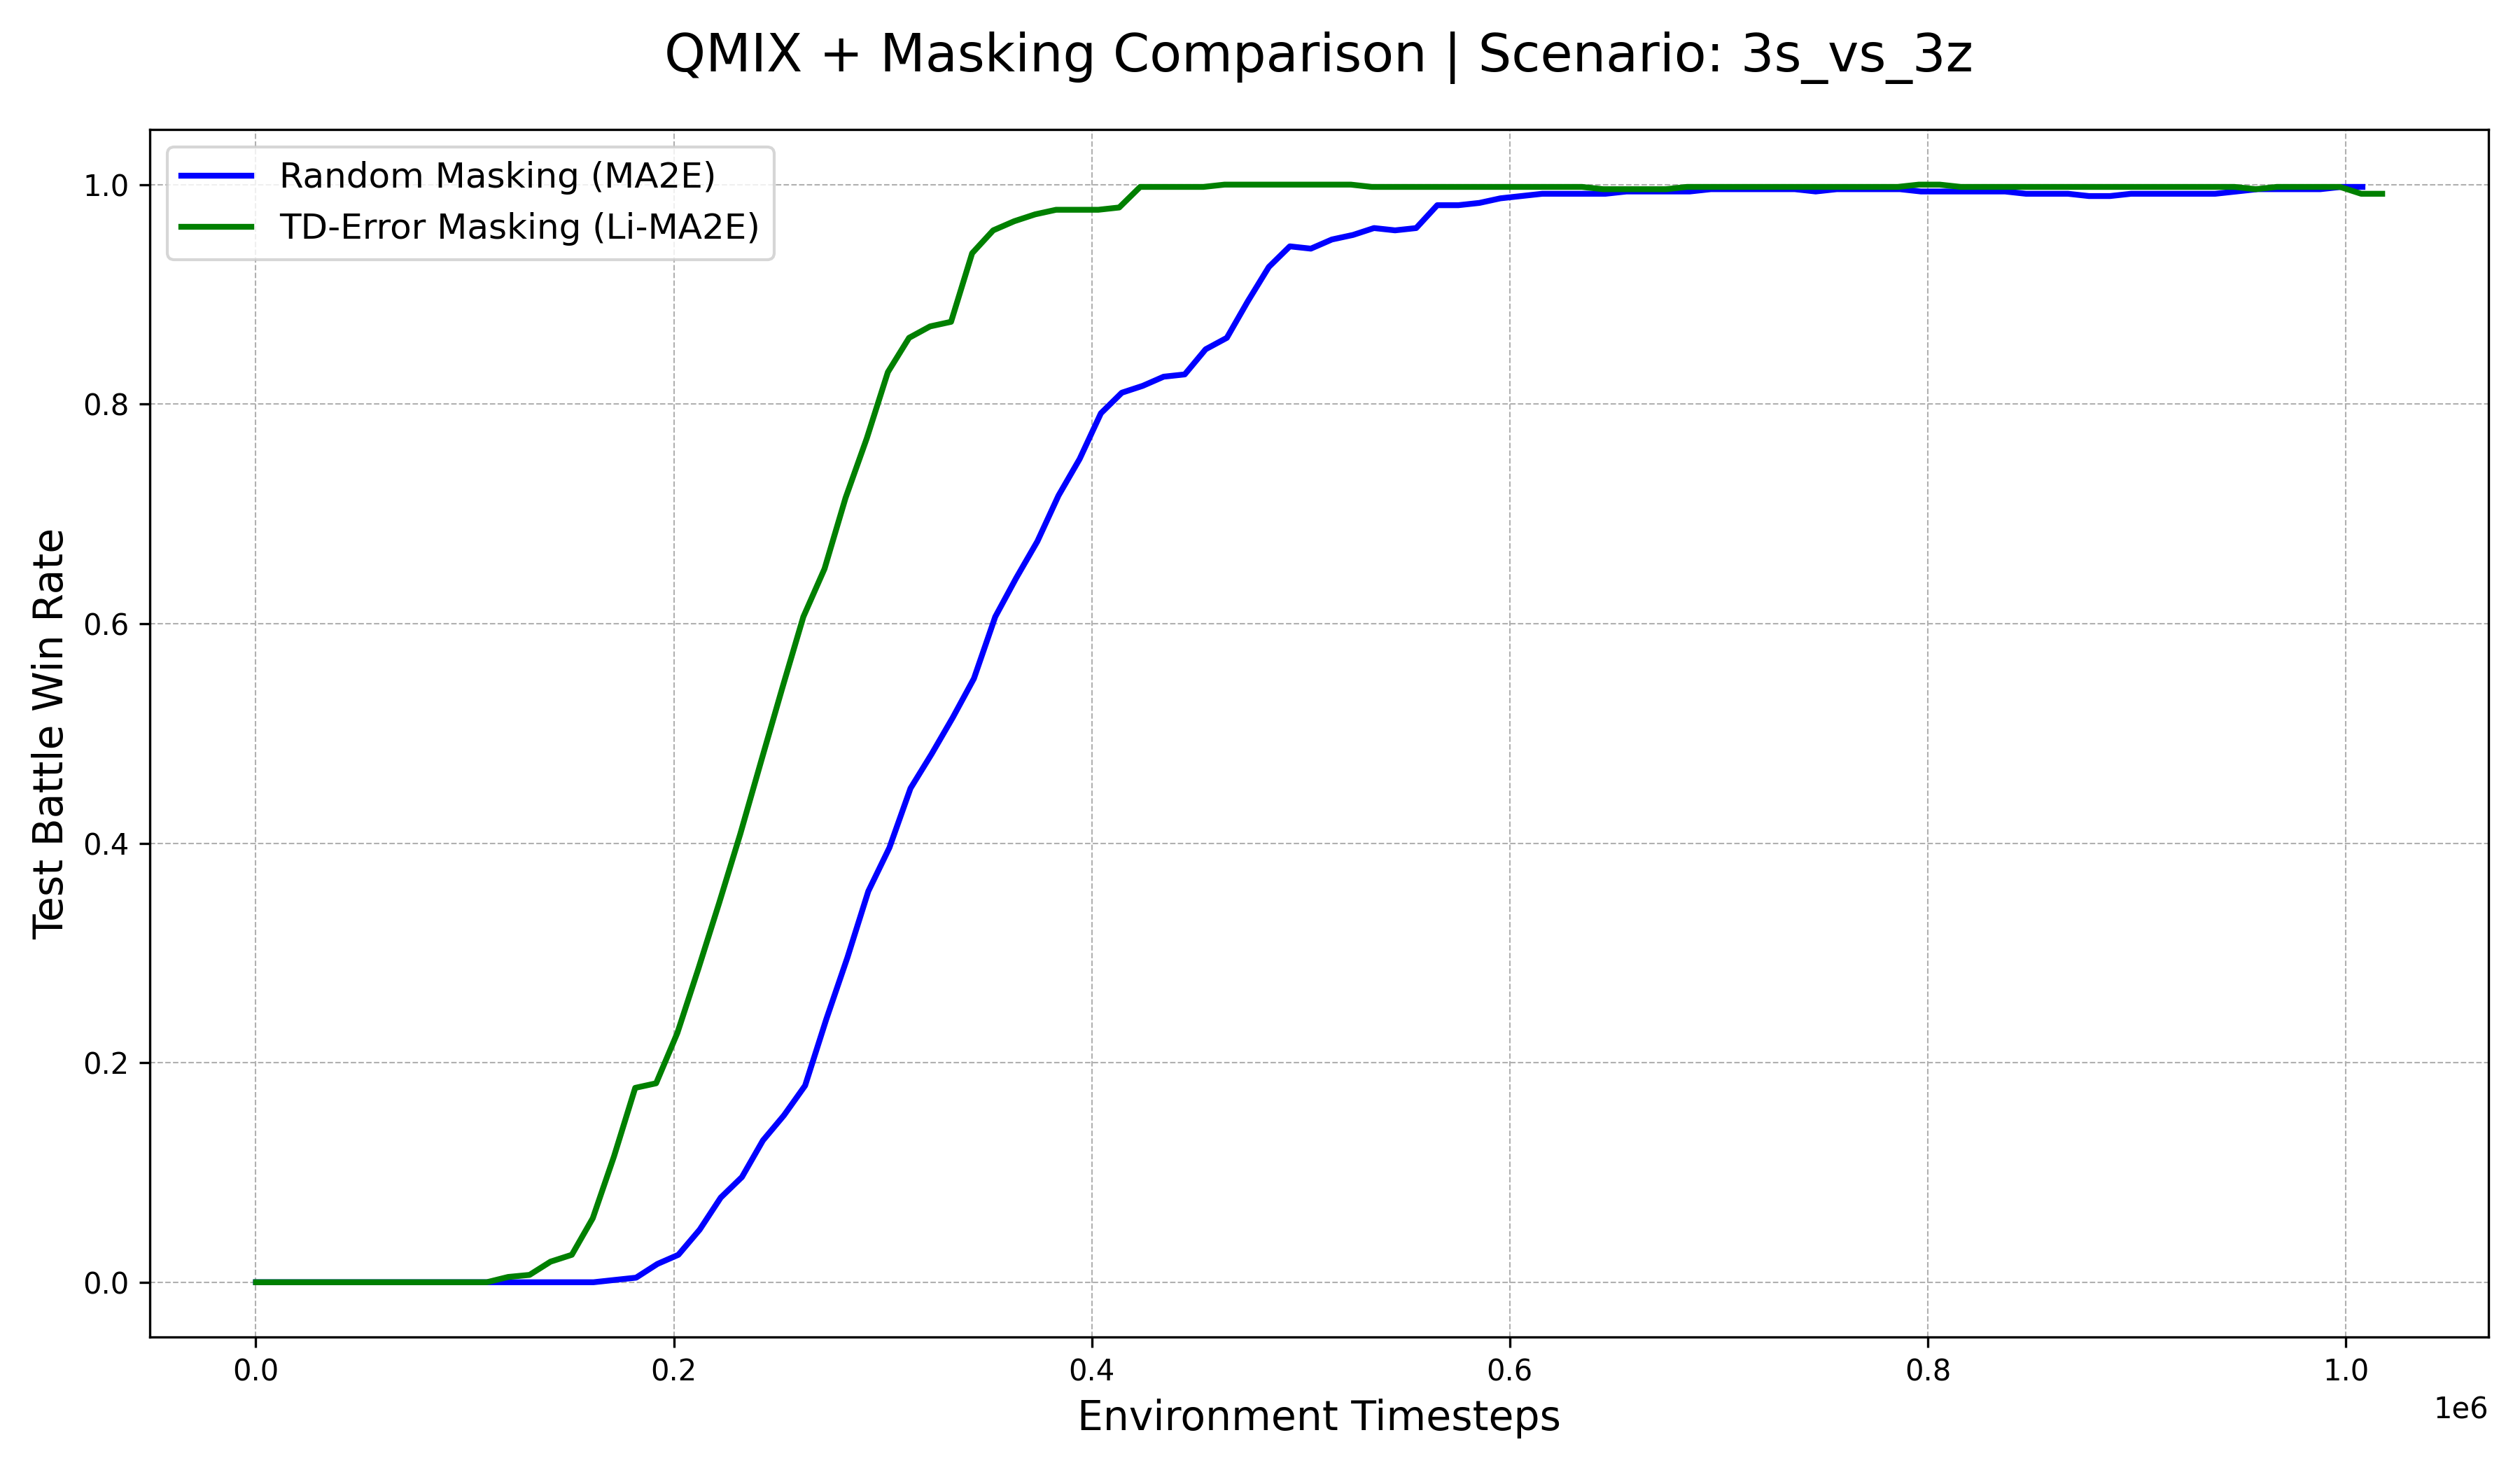
\includegraphics[width=0.8\textwidth]{images_pfe/results_li-ma2e/comparison_plot_3s_vs_3z.png}
%     \caption{Performance comparison on the \texttt{3s\_vs\_3z} SMAC map. LI-MA2E demonstrates significantly improved sample efficiency over the baseline.}
%     \label{fig:3s_vs_3z}
% \end{figure}

% \paragraph{Analysis}
% In the \texttt{3s\_vs\_3z} scenario, the benefit of our LI-MA2E framework becomes immediately apparent. As shown in Figure~\ref{fig:3s_vs_3z}, the agent guided by TD-Error Masking (green line) learns significantly faster than the baseline agent using Random Masking (blue line).

% Our method begins to achieve a non-zero win rate earlier, and its learning curve is considerably steeper, indicating superior sample efficiency. The LI-MA2E agent reaches a perfect win rate at approximately 400,000 timesteps, while the baseline requires around 600,000 timesteps to achieve the same level of performance. This result supports our hypothesis that as scenario complexity increases, an intelligent masking strategy that focuses the MAE's representational power on poorly performing agents provides a distinct advantage, enabling the system to solve the coordination task more rapidly.
% \subsubsection{Scenario: \texttt{3s\_vs\_4z}}

% Now, we test a harder scenario called \texttt{3s\_vs\_4z}. Here, our \textbf{3 Stalker agents}, who can shoot from a distance, must fight against \textbf{4 enemy Zealot units}, which are durable but can only attack up close.

% This test is much more difficult because our agents are \textbf{outnumbered}. To win, they must use two skills together perfectly:
% \begin{enumerate}
%     \item \textbf{Kiting:} They must keep running away from the Zealots to stay safe, while stopping to shoot them.
%     \item \textbf{Focus-Firing:} All three Stalkers must attack the \textit{same} Zealot at the same time to defeat it as quickly as possible.
% \end{enumerate}
% This requires excellent teamwork to succeed. The results of this difficult test are shown in Figure~\ref{fig:3s_vs_4z}.

% \begin{figure}[h]
%     \centering
%      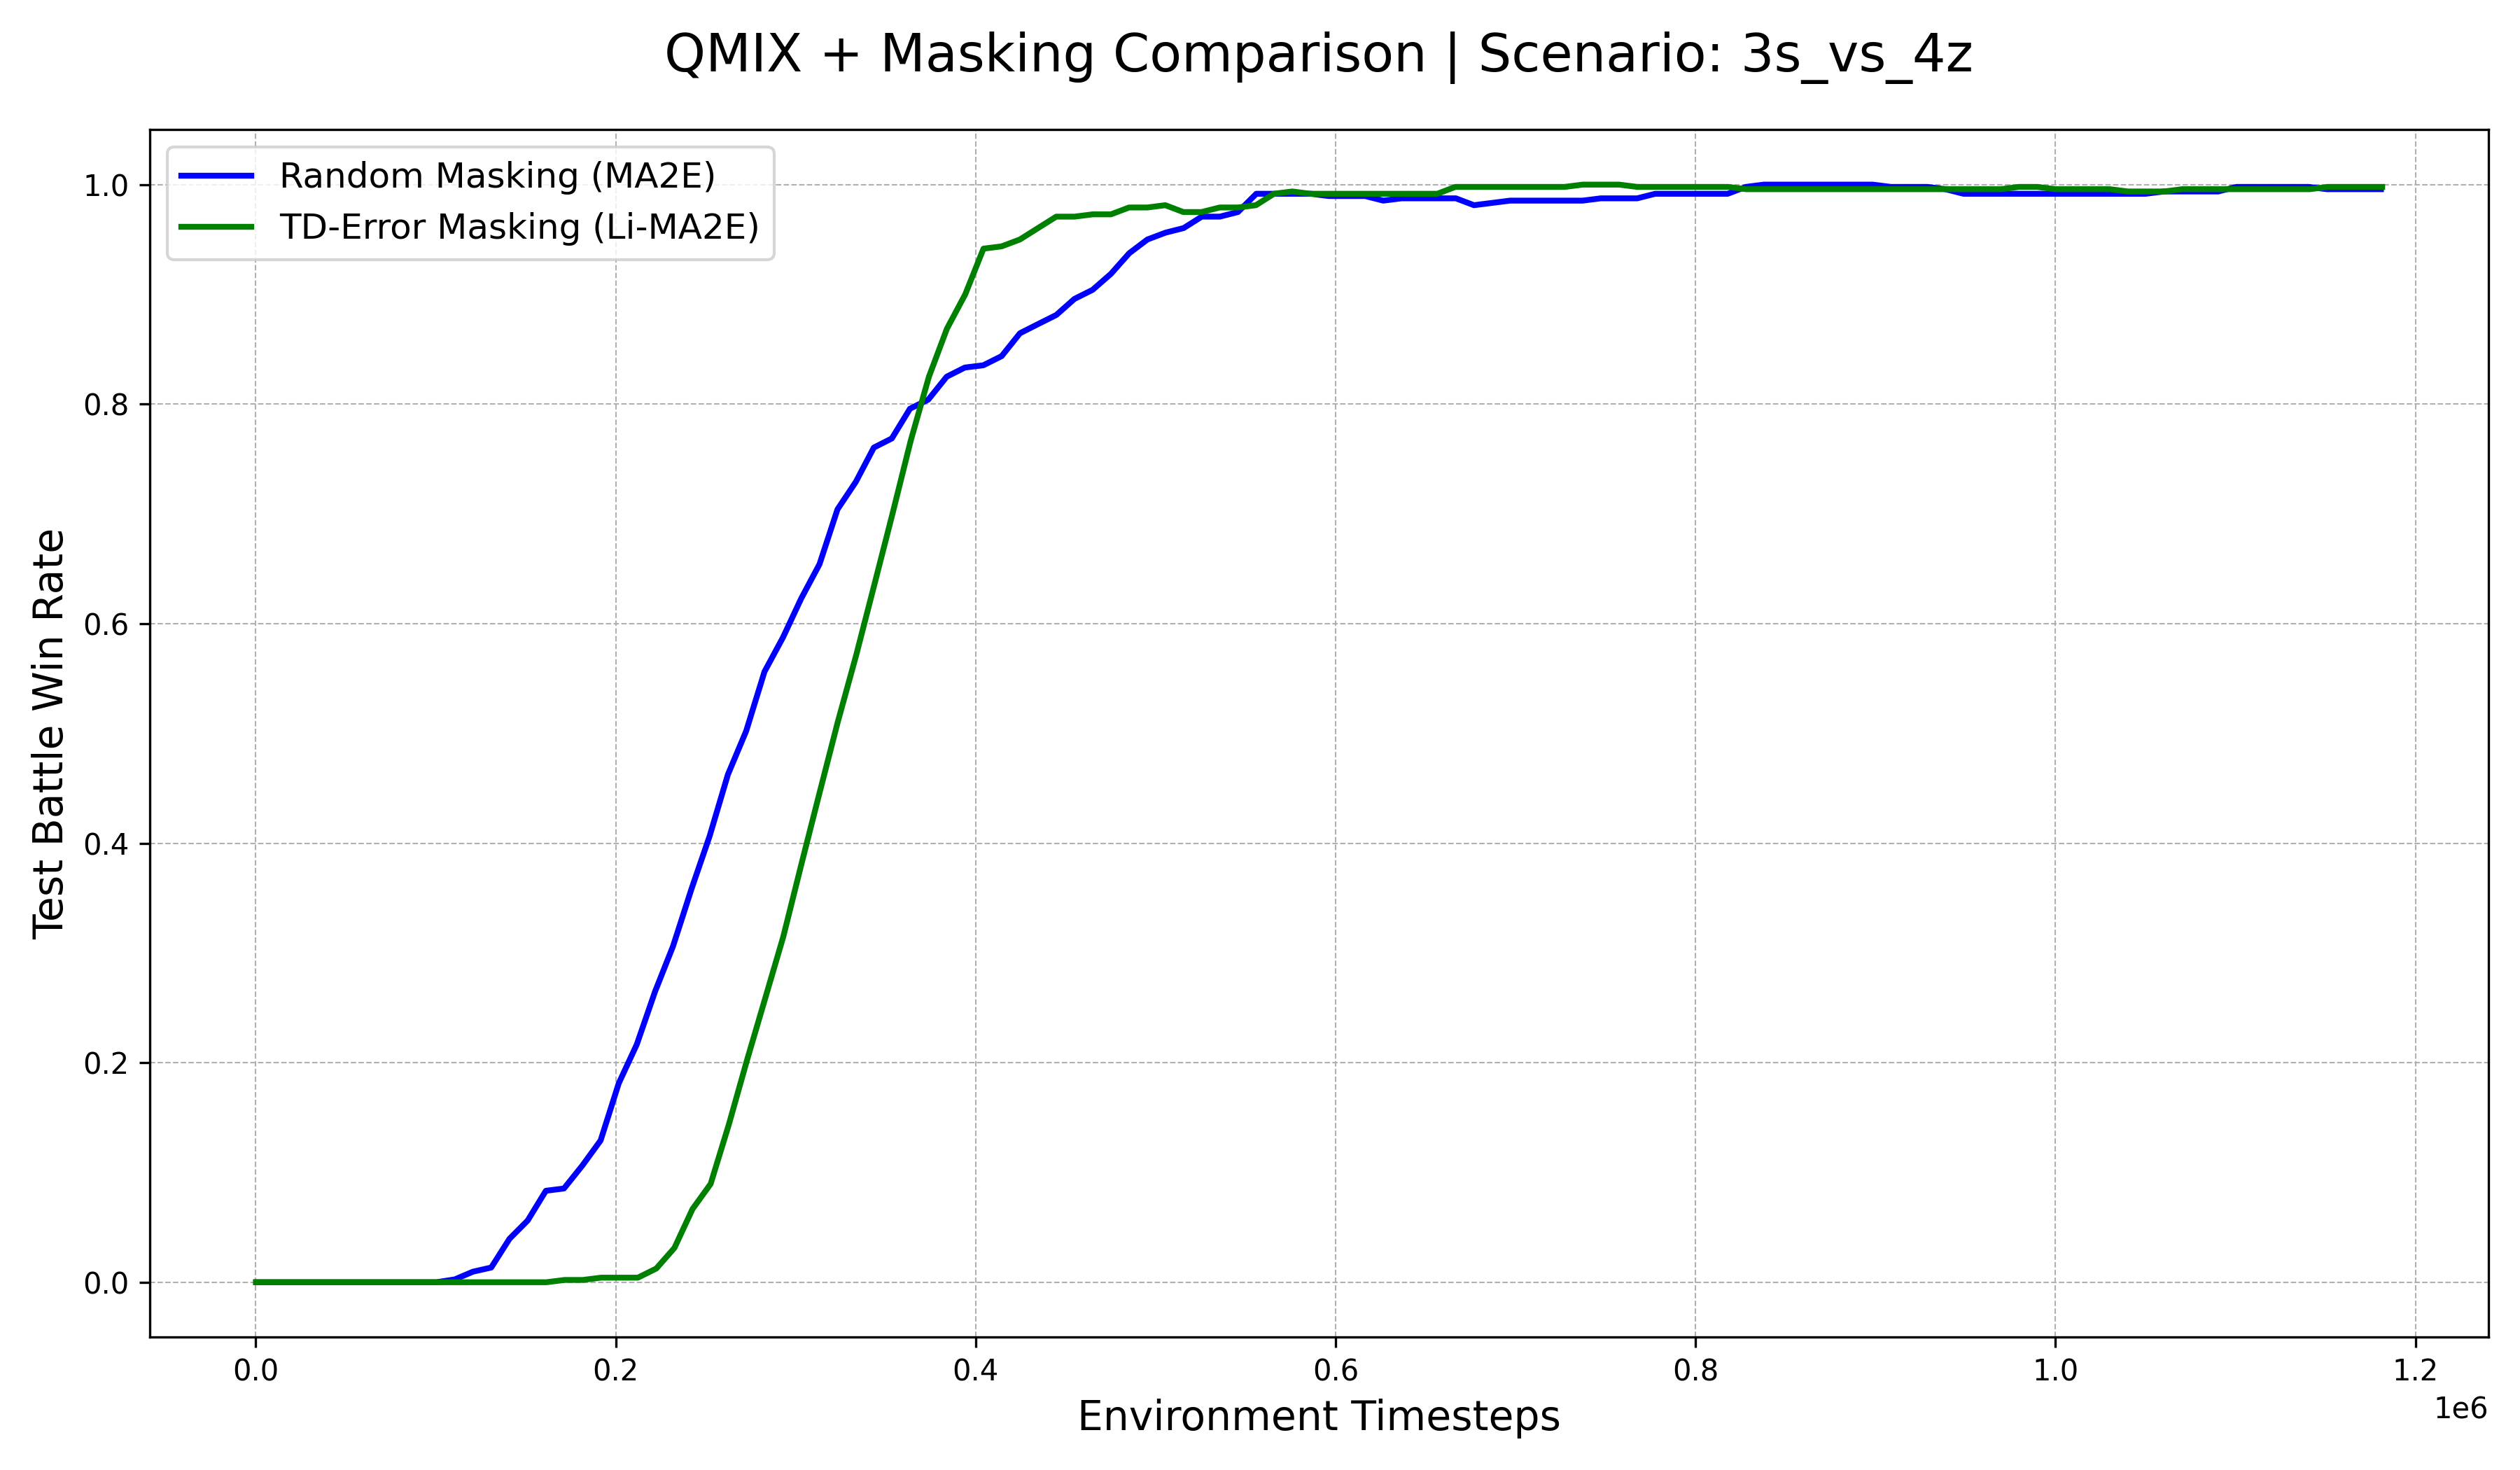
\includegraphics[width=0.8\textwidth]{images_pfe/results_li-ma2e/comparison_plot_3s_vs_4z.png}
%     \caption{Performance comparison on the \texttt{3s\_vs\_4z} SMAC map. The plot shows a trade-off between the faster initial learning of the baseline and the more stable final convergence of LI-MA2E.}
%     \label{fig:3s_vs_4z}
% \end{figure}

% \paragraph{Analysis}
% The \texttt{3s\_vs\_4z} scenario reveals an interesting trade-off between learning speed and final policy stability. As shown in Figure~\ref{fig:3s_vs_4z}, the baseline MA2E with Random Masking (blue line) exhibits a faster initial learning curve, reaching a high win rate more quickly.

% However, a closer look at the convergence phase (after 0.6 million timesteps) shows that our LI-MA2E framework (green line) achieves a more stable and decisive convergence at a 100\% win rate. The baseline's performance, in contrast, shows more fluctuation before finally settling. This suggests that while the exploratory nature of random masking may find a working solution faster in this specific scenario, the guided approach of LI-MA2E produces a more robust and stable final policy.


% \subsubsection{Scenario: \texttt{3s\_vs\_5z}}

% Next, we test our method on \texttt{3s\_vs\_5z}, a very hard challenge from the \texttt{HARD} difficulty category. In this test, our \textbf{3 Stalker agents} (who shoot from a distance) are heavily outnumbered by \textbf{5 durable enemy Zealots} (who attack up close).

% To win this difficult fight, the agents must be perfect at two skills at the same time:
% \begin{enumerate}
%     \item \textbf{Kiting:} They must always keep running away from the Zealots to avoid taking damage, while still turning to shoot.
%     \item \textbf{Focus-Firing:} All three of our agents must attack the exact same enemy at the same time. This is the only way to defeat one of the five enemies quickly.
% \end{enumerate}
% This is a major test of teamwork. If even one agent makes a mistake, the team will likely lose. The agents must learn to coordinate perfectly to survive and win. The results for this difficult test are shown in Figure~\ref{fig:3s_vs_5z}.

% \begin{figure}[h]
%     \centering
%     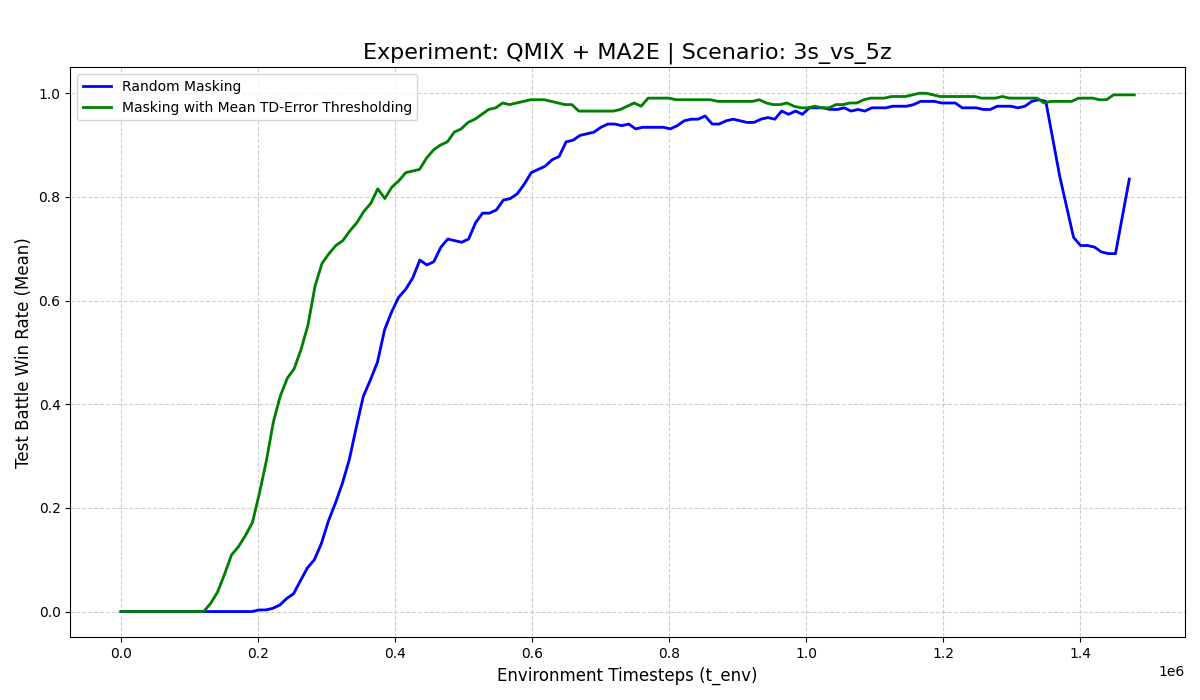
\includegraphics[width=0.8\textwidth]{images_pfe/results_li-ma2e/test_battle_won_mean_3s_vs_5z_Mean_TD-Error_Thresholding _smoothed.png}
%     \caption{Performance comparison on the \texttt{3s\_vs\_5z} HARD scenario. In this complex asymmetric task, LI-MA2E demonstrates vastly superior sample efficiency and produces a more stable final policy compared to the baseline Random Masking.}
%     \label{fig:3s_vs_5z}
% \end{figure}

% \paragraph{Analysis}
% In stark contrast to the previous map, the results on \texttt{3s\_vs\_5z} show a clear and significant advantage for our LI-MA2E framework (green line). The intelligent masking strategy leads to a dramatic improvement in both sample efficiency and final policy stability.

% LI-MA2E learns much faster, achieving a near-perfect win rate before 0.6 million timesteps, while the baseline with random masking (blue line) requires more than 1.2 million timesteps to reach a similar peak performance. Crucially, during the later stages of training (after 1.3 million steps), the baseline policy exhibits significant instability with a sharp drop in performance, a behavior not observed in our method.

% This strong result supports our core hypothesis. The \texttt{3s\_vs\_5z} map requires precise, coordinated kiting, where a single agent's mistake can be catastrophic. By adaptively focusing the MAE's reconstruction on the agent with the highest immediate error, our framework helps the team learn this essential cooperative strategy more effectively and robustly. The final stability of the LI-MA2E policy suggests that it has discovered a more general and resilient solution compared to the brittle policy learned by the baseline.

% \subsubsection{Scenario: \texttt{8m}}
% We continue our evaluation with the \texttt{8m} scenario, a symmetric map which pits \textbf{8 allied Marines against 8 enemy Marines}. This task increases the number of homogeneous agents compared to \texttt{3m} and demands effective \textbf{focus-firing} to succeed. Focus-firing is a critical coordination strategy where multiple agents target and eliminate a single enemy unit at a time. This tactic maximizes the applied damage and removes sources of enemy fire from the battlefield as quickly as possible, representing a significant coordination challenge for a multi-agent system. The results are presented in Figure~\ref{fig:8m}.

% \begin{figure}[h]
%     \centering
%     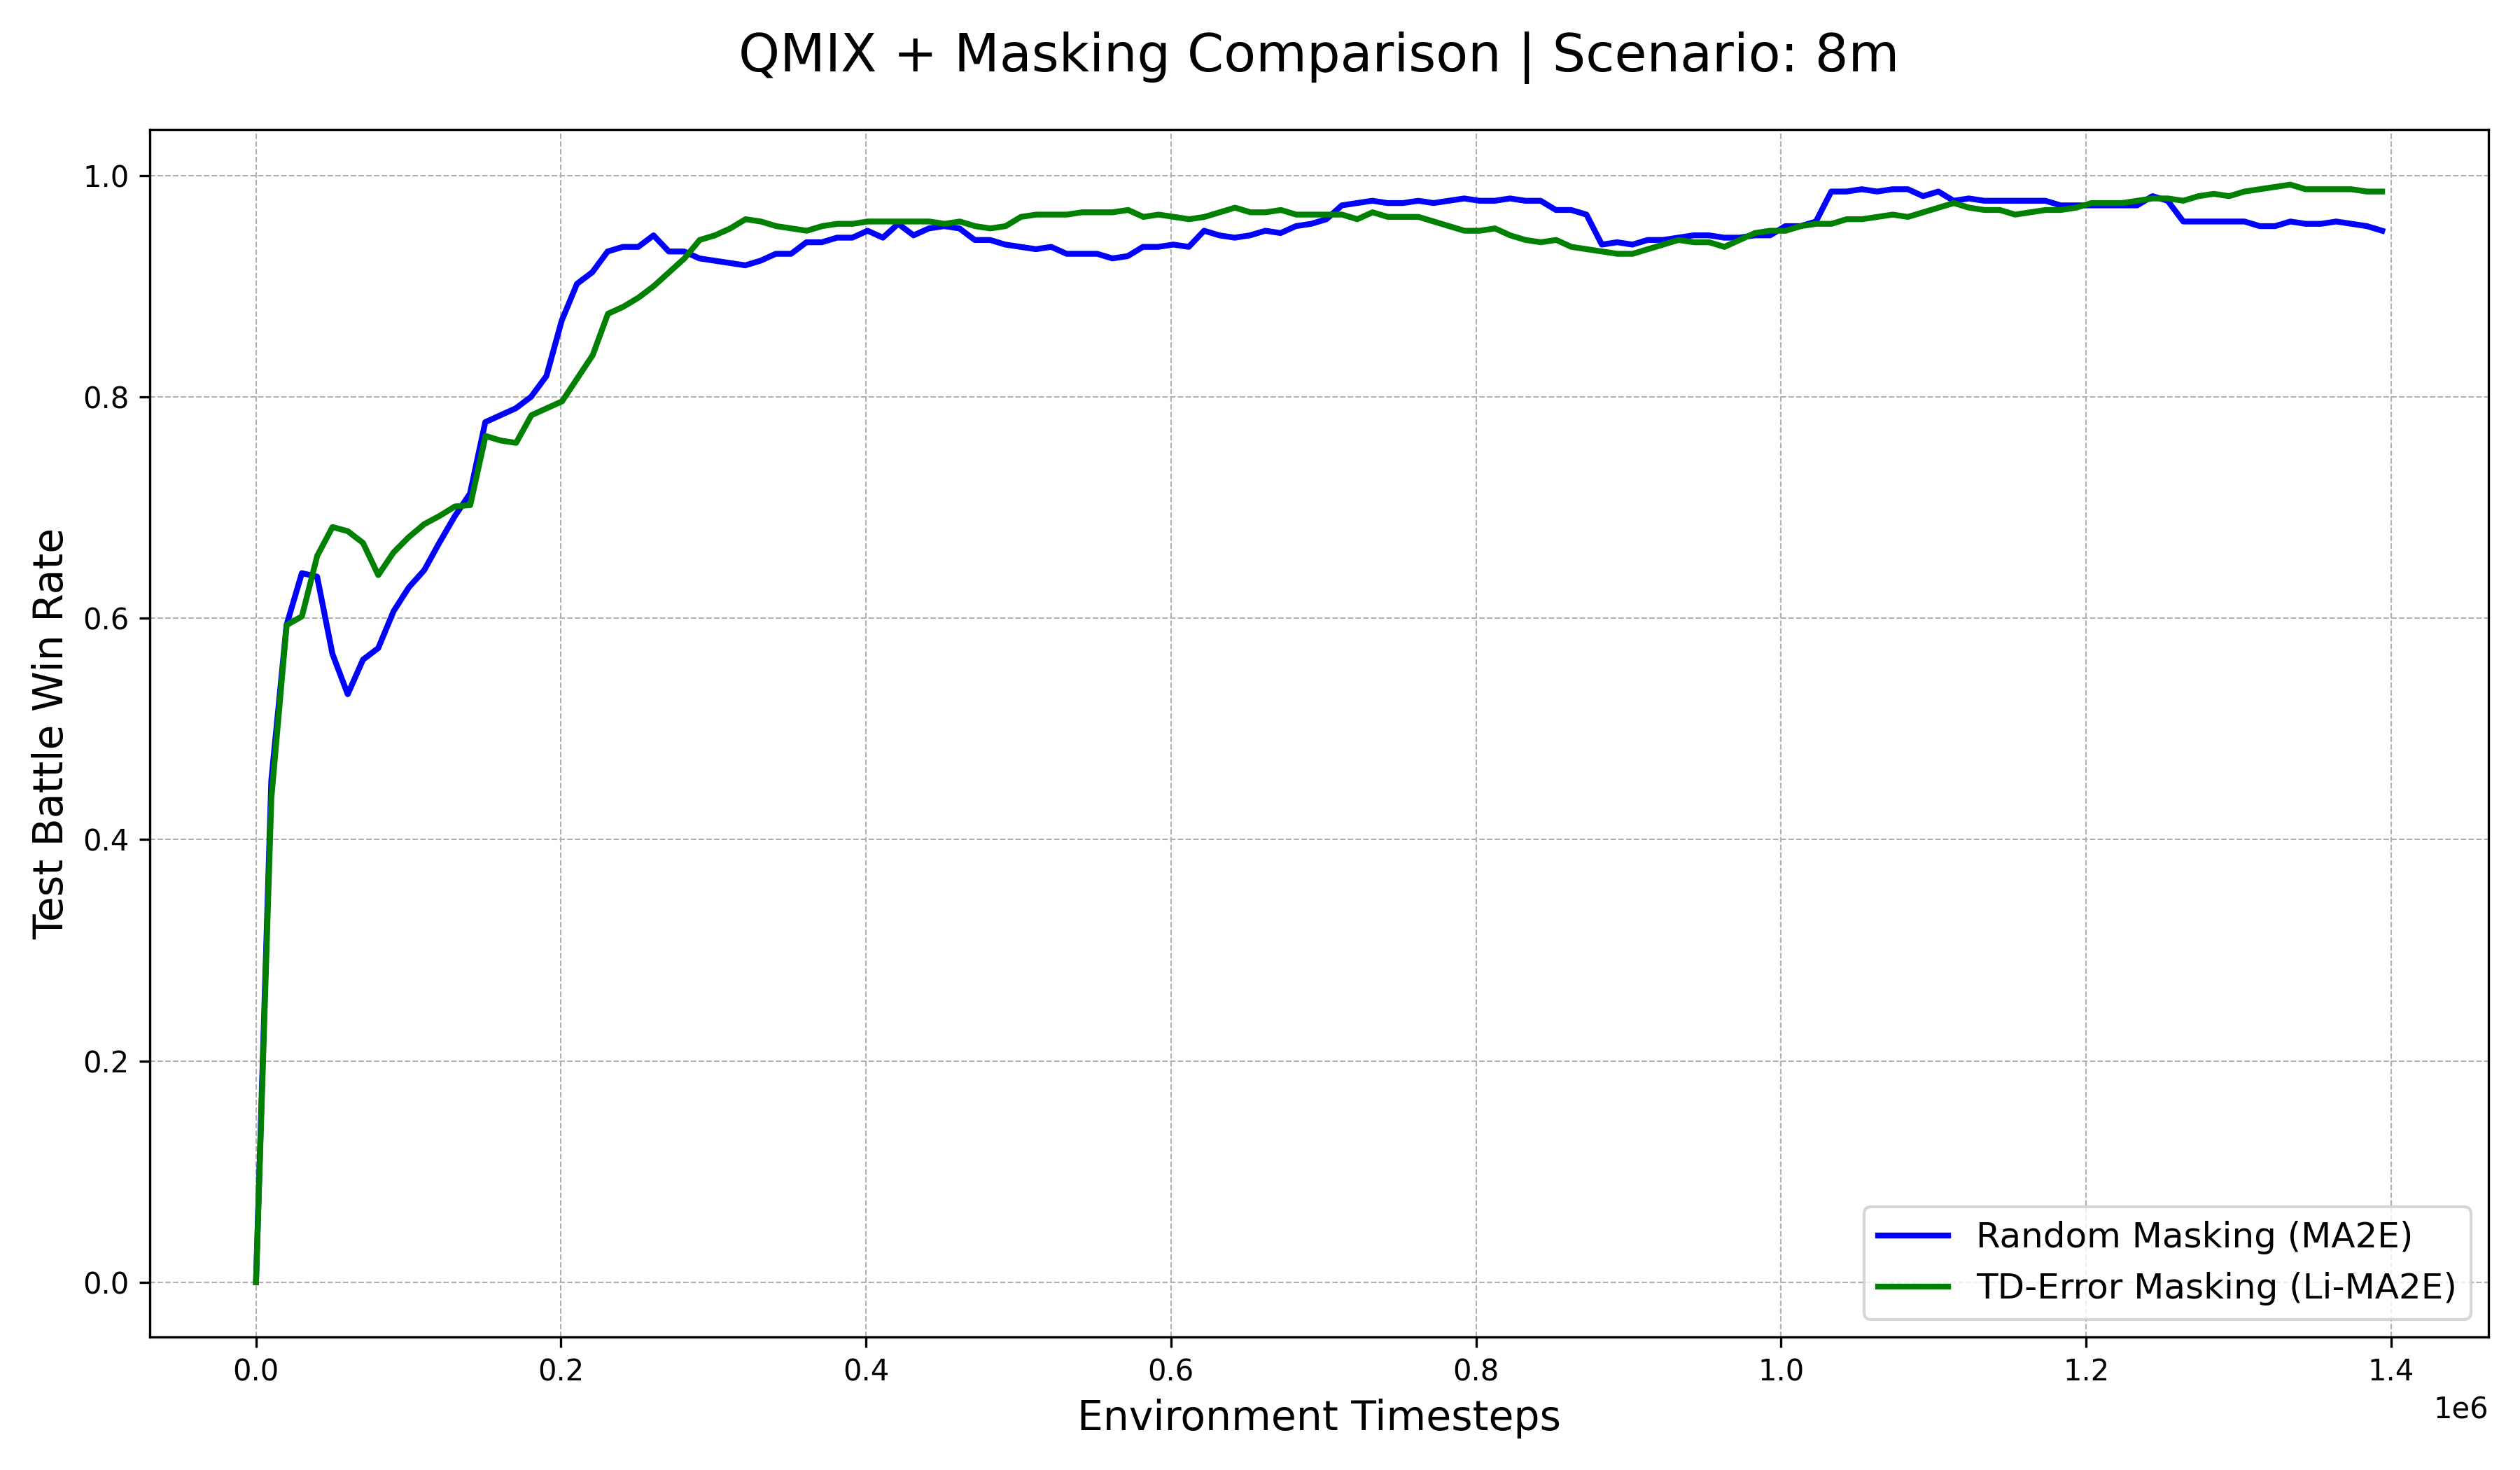
\includegraphics[width=0.8\textwidth]{images_pfe/results_li-ma2e/comparison_plot_8m.png}
%     \caption{Performance comparison on the \texttt{8m} SMAC map. Both methods converge to a perfect win rate, with the baseline showing a faster initial learning rate.}
%     \label{fig:8m}
% \end{figure}
% \paragraph{Analysis}
% Upon careful re-examination of the provided plot for the \texttt{8m} scenario, the results show a nuanced competition between the two methods. The baseline Random Masking (blue line) demonstrates a higher sample efficiency during the initial critical learning phase.

% As seen in Figure~\ref{fig:8m}, the blue line's win rate rises more steeply and consistently between 0.1 million and 0.3 million timesteps, reaching a high level of performance first. The LI-MA2E method (green line), while also learning the task, shows a noticeable dip in performance around 0.15 million timesteps and follows a slower learning trajectory in this initial phase. Both methods do eventually converge to a near-perfect win rate after approximately 1.0 million timesteps, showing that both can ultimately solve this scenario. However, the advantage in learning speed in this case belongs to the baseline.

% This finding suggests that in this specific homogeneous scenario with a larger number of agents, the broader, exploratory nature of random masking may be more effective at building a general representation than the more focused TD-error approach. This helps to define the conditions under which our LI-MA2E provides the most significant advantage—namely, in more complex, asymmetric scenarios.
\section{Main Results: Comparative Performance of $LI-{MA}^2E$}
\label{sec:main_results}

Having established the superiority of our Adaptive Mean TD-Error Thresholding strategy in the previous section, we now present a comprehensive performance evaluation of the final $LI-{MA}^2E$ framework. To validate its effectiveness and generalization capabilities, we benchmark our method against the baseline ${MA}^2E$ with random masking across a suite of challenging HARD, MEDIUM, and EASY scenarios from the SMAC environment. This section is structured to answer key research questions regarding our method's effectiveness, policy quality, and underlying learning dynamics.

\subsection{RQ1: Does Learning-Informed Masking Improve Task Completion Success?}

To answer this question, we evaluate the primary metric for task success in SMAC: the \textbf{test battle win rate}. This metric measures the percentage of episodes in which the allied agents successfully completed their objective. We present a detailed, scenario-by-scenario analysis below.
\subsubsection{Scenario: \texttt{3m}}
Our first evaluation is on the \texttt{3m} scenario, a simple symmetric map that pits \textbf{3 allied Marines against three enemy Marines}. Because  \textbf{the agents are homogeneous} and the \textbf{setup is symmetric}, the primary challenge in this map is learning a fundamental cooperative tactic: \textbf{focus-firing}. To win consistently, all three agents must learn to coordinate their attacks on the same enemy target at the same time to eliminate it quickly, rather than spreading their damage ineffectually across multiple targets. This scenario serves as a basic test of coordination. The results are presented in Figure~\ref{fig:3m}.

\begin{figure}[h]
    \centering
    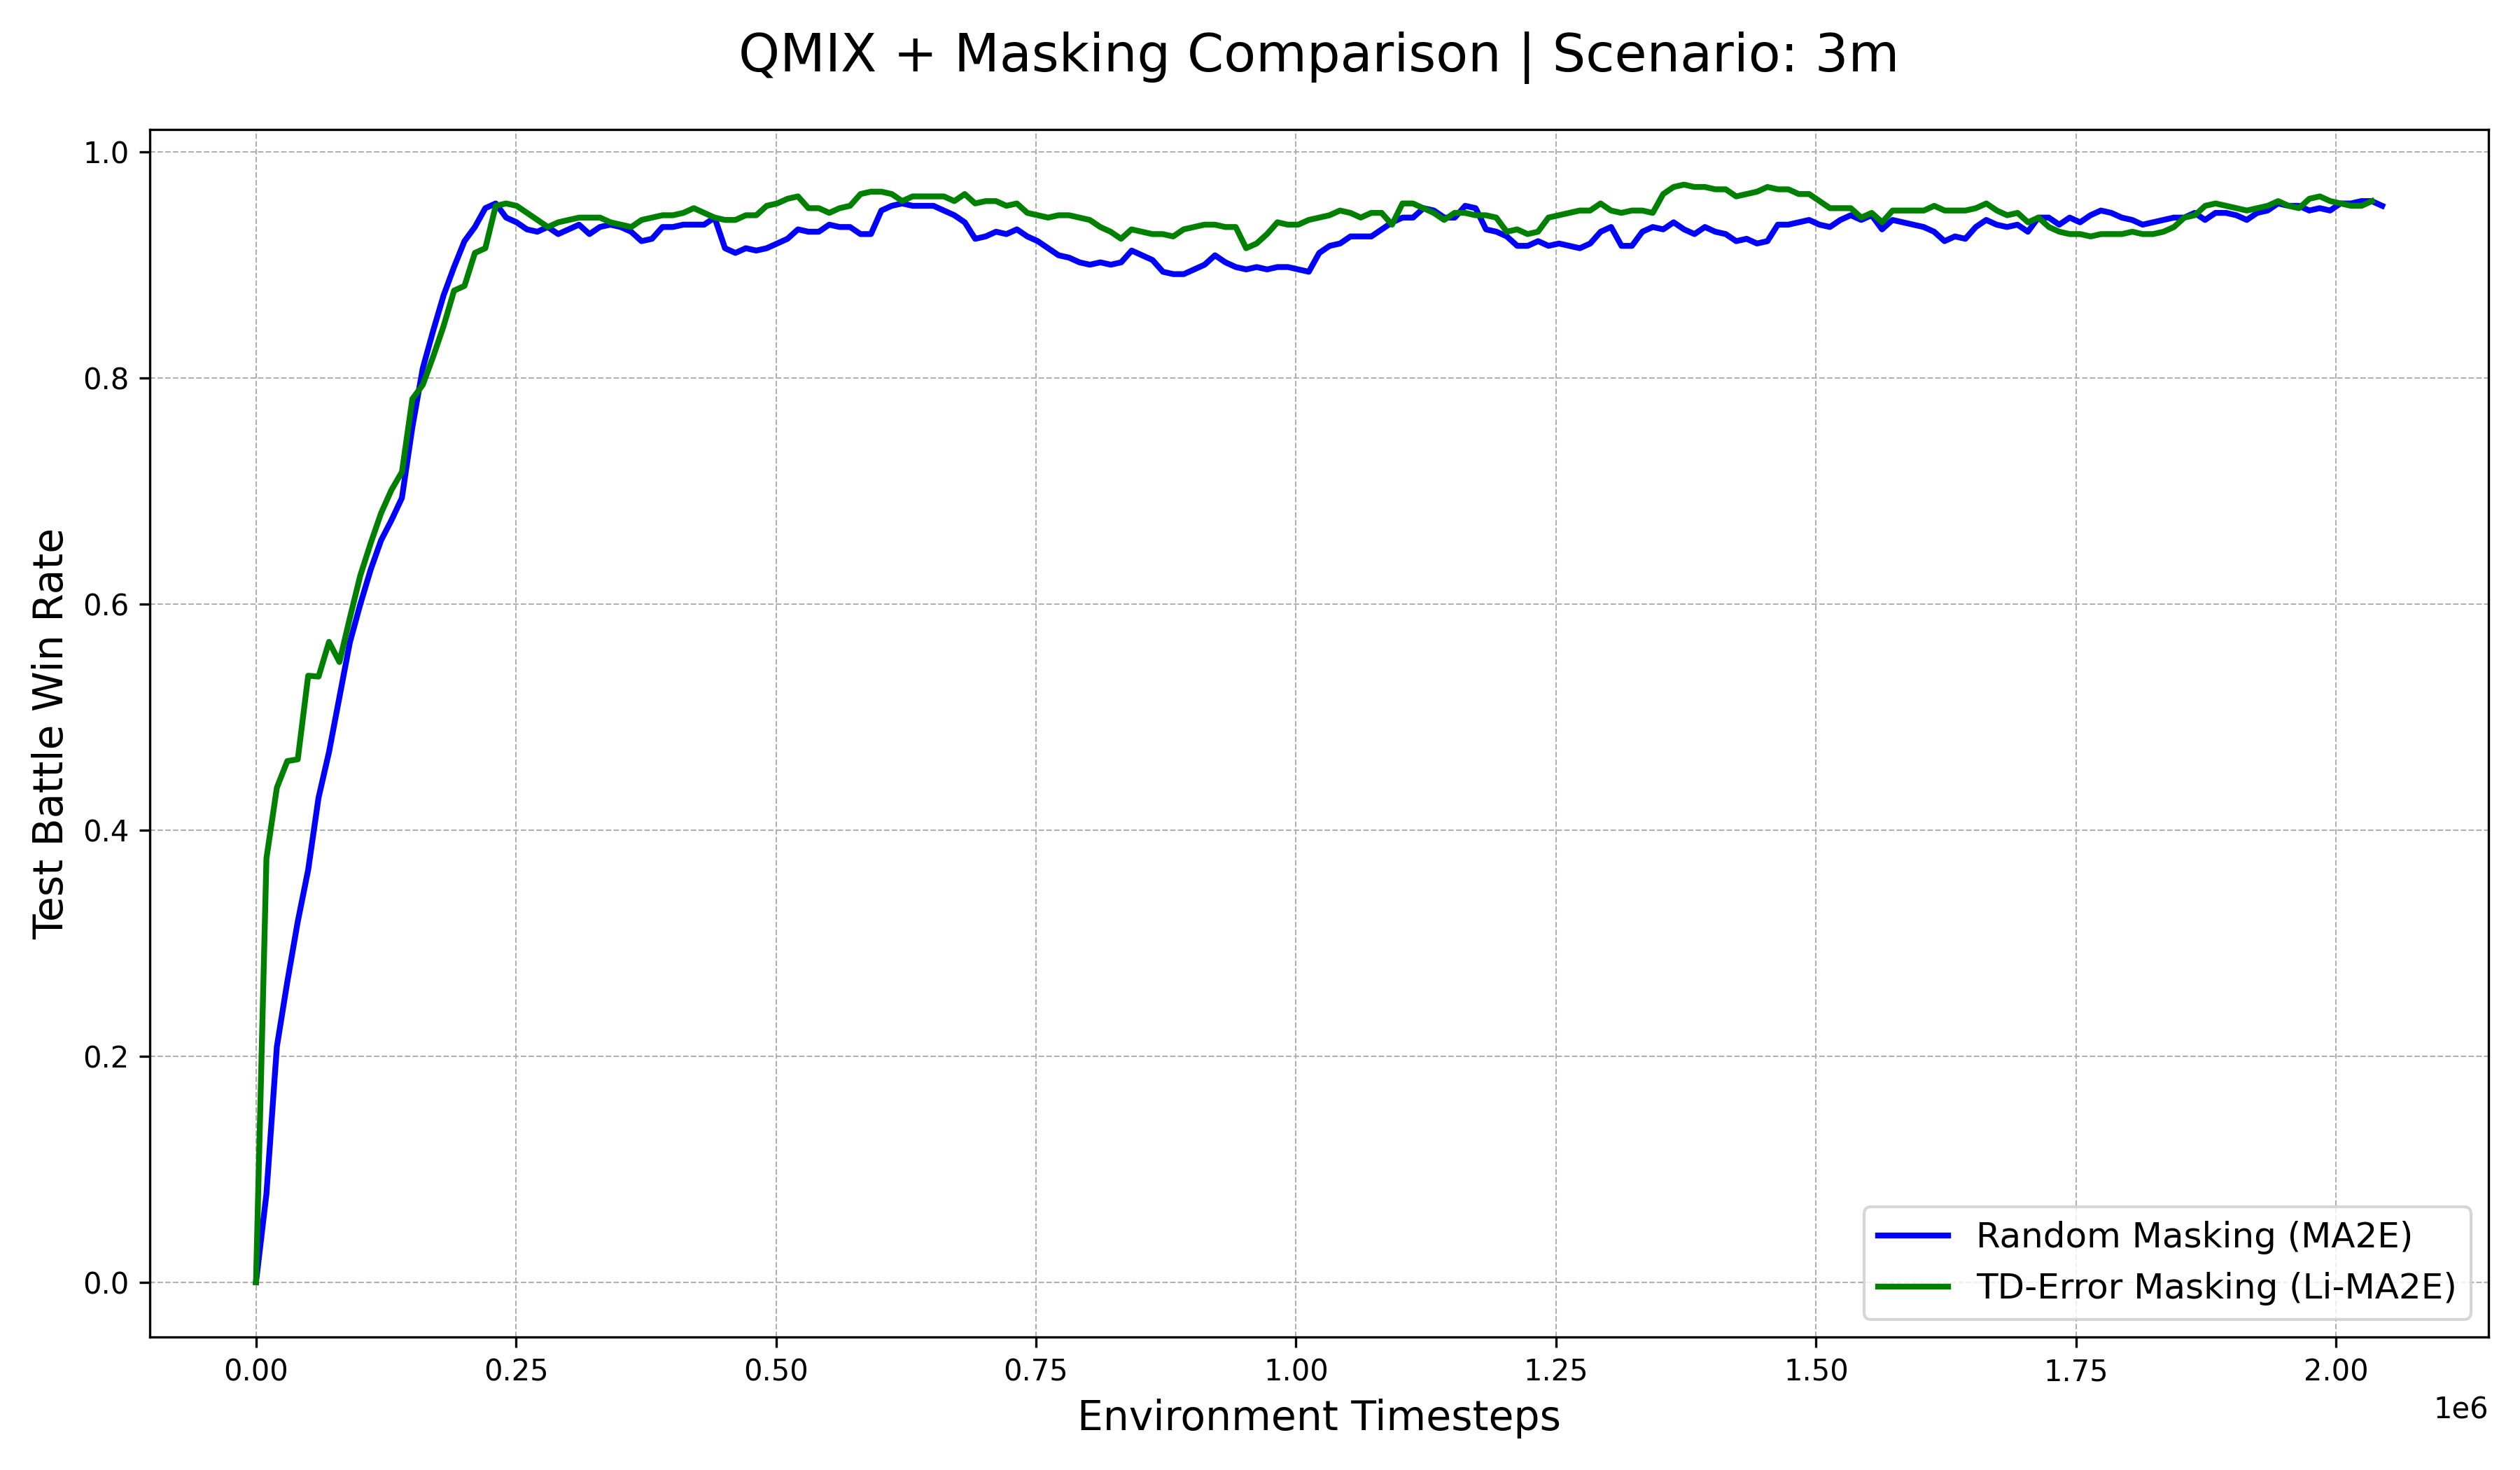
\includegraphics[width=0.8\textwidth]{images_pfe/results_li-ma2e/comparison_plot_3m.png}
    \caption{Performance comparison on the \texttt{3m} SMAC map. On this simple symmetric scenario, the performance of $LI-{MA}^2E$ is comparable to the random masking baseline.}
    \label{fig:3m}
\end{figure}

\paragraph{Analysis}
As the learning curves in Figure~\ref{fig:3m} show, the performance of our $LI-{MA}^2E$ framework (green line) is largely comparable to that of the baseline ${MA}^2E$ with random masking (blue line). Both methods learn the task very rapidly, achieving a near-perfect win rate in under 250,000 environment timesteps. Throughout the remainder of the training, both policies maintain a similar high level of performance.
This result suggests that in simpler scenarios where the need for complex coordination to overcome partial observability is low, the additional guidance provided by our intelligent masking strategy does not yield a significant advantage. The baseline random masking is sufficient for the MAE module to learn the necessary representations to solve this task effectively. This provides an important baseline, demonstrating that our method's complexity does not hinder performance on easy tasks while setting the stage for evaluation on more demanding scenarios.

\subsubsection{Scenario: \texttt{3s\_vs\_3z}}
Next, we look at the \texttt{3s\_vs\_3z} scenario. In this test, our \textbf{3 agents control Stalker units}, which can attack from a distance. They face \textbf{3 enemy Zealot units}, which are severe but can only attack up close.

Because our agents can shoot from far away, the most important skill they must learn is called \textbf{kiting}. Kiting means the Stalkers must keep moving away from the chasing Zealots, while stopping briefly to shoot at them. The goal is to damage the enemy without letting them get close enough to hit back. To do this well, all three of our agents need to work together as a team. The results of this test are shown in Figure~\ref{fig:3s_vs_3z}.

\begin{figure}[h]
    \centering
    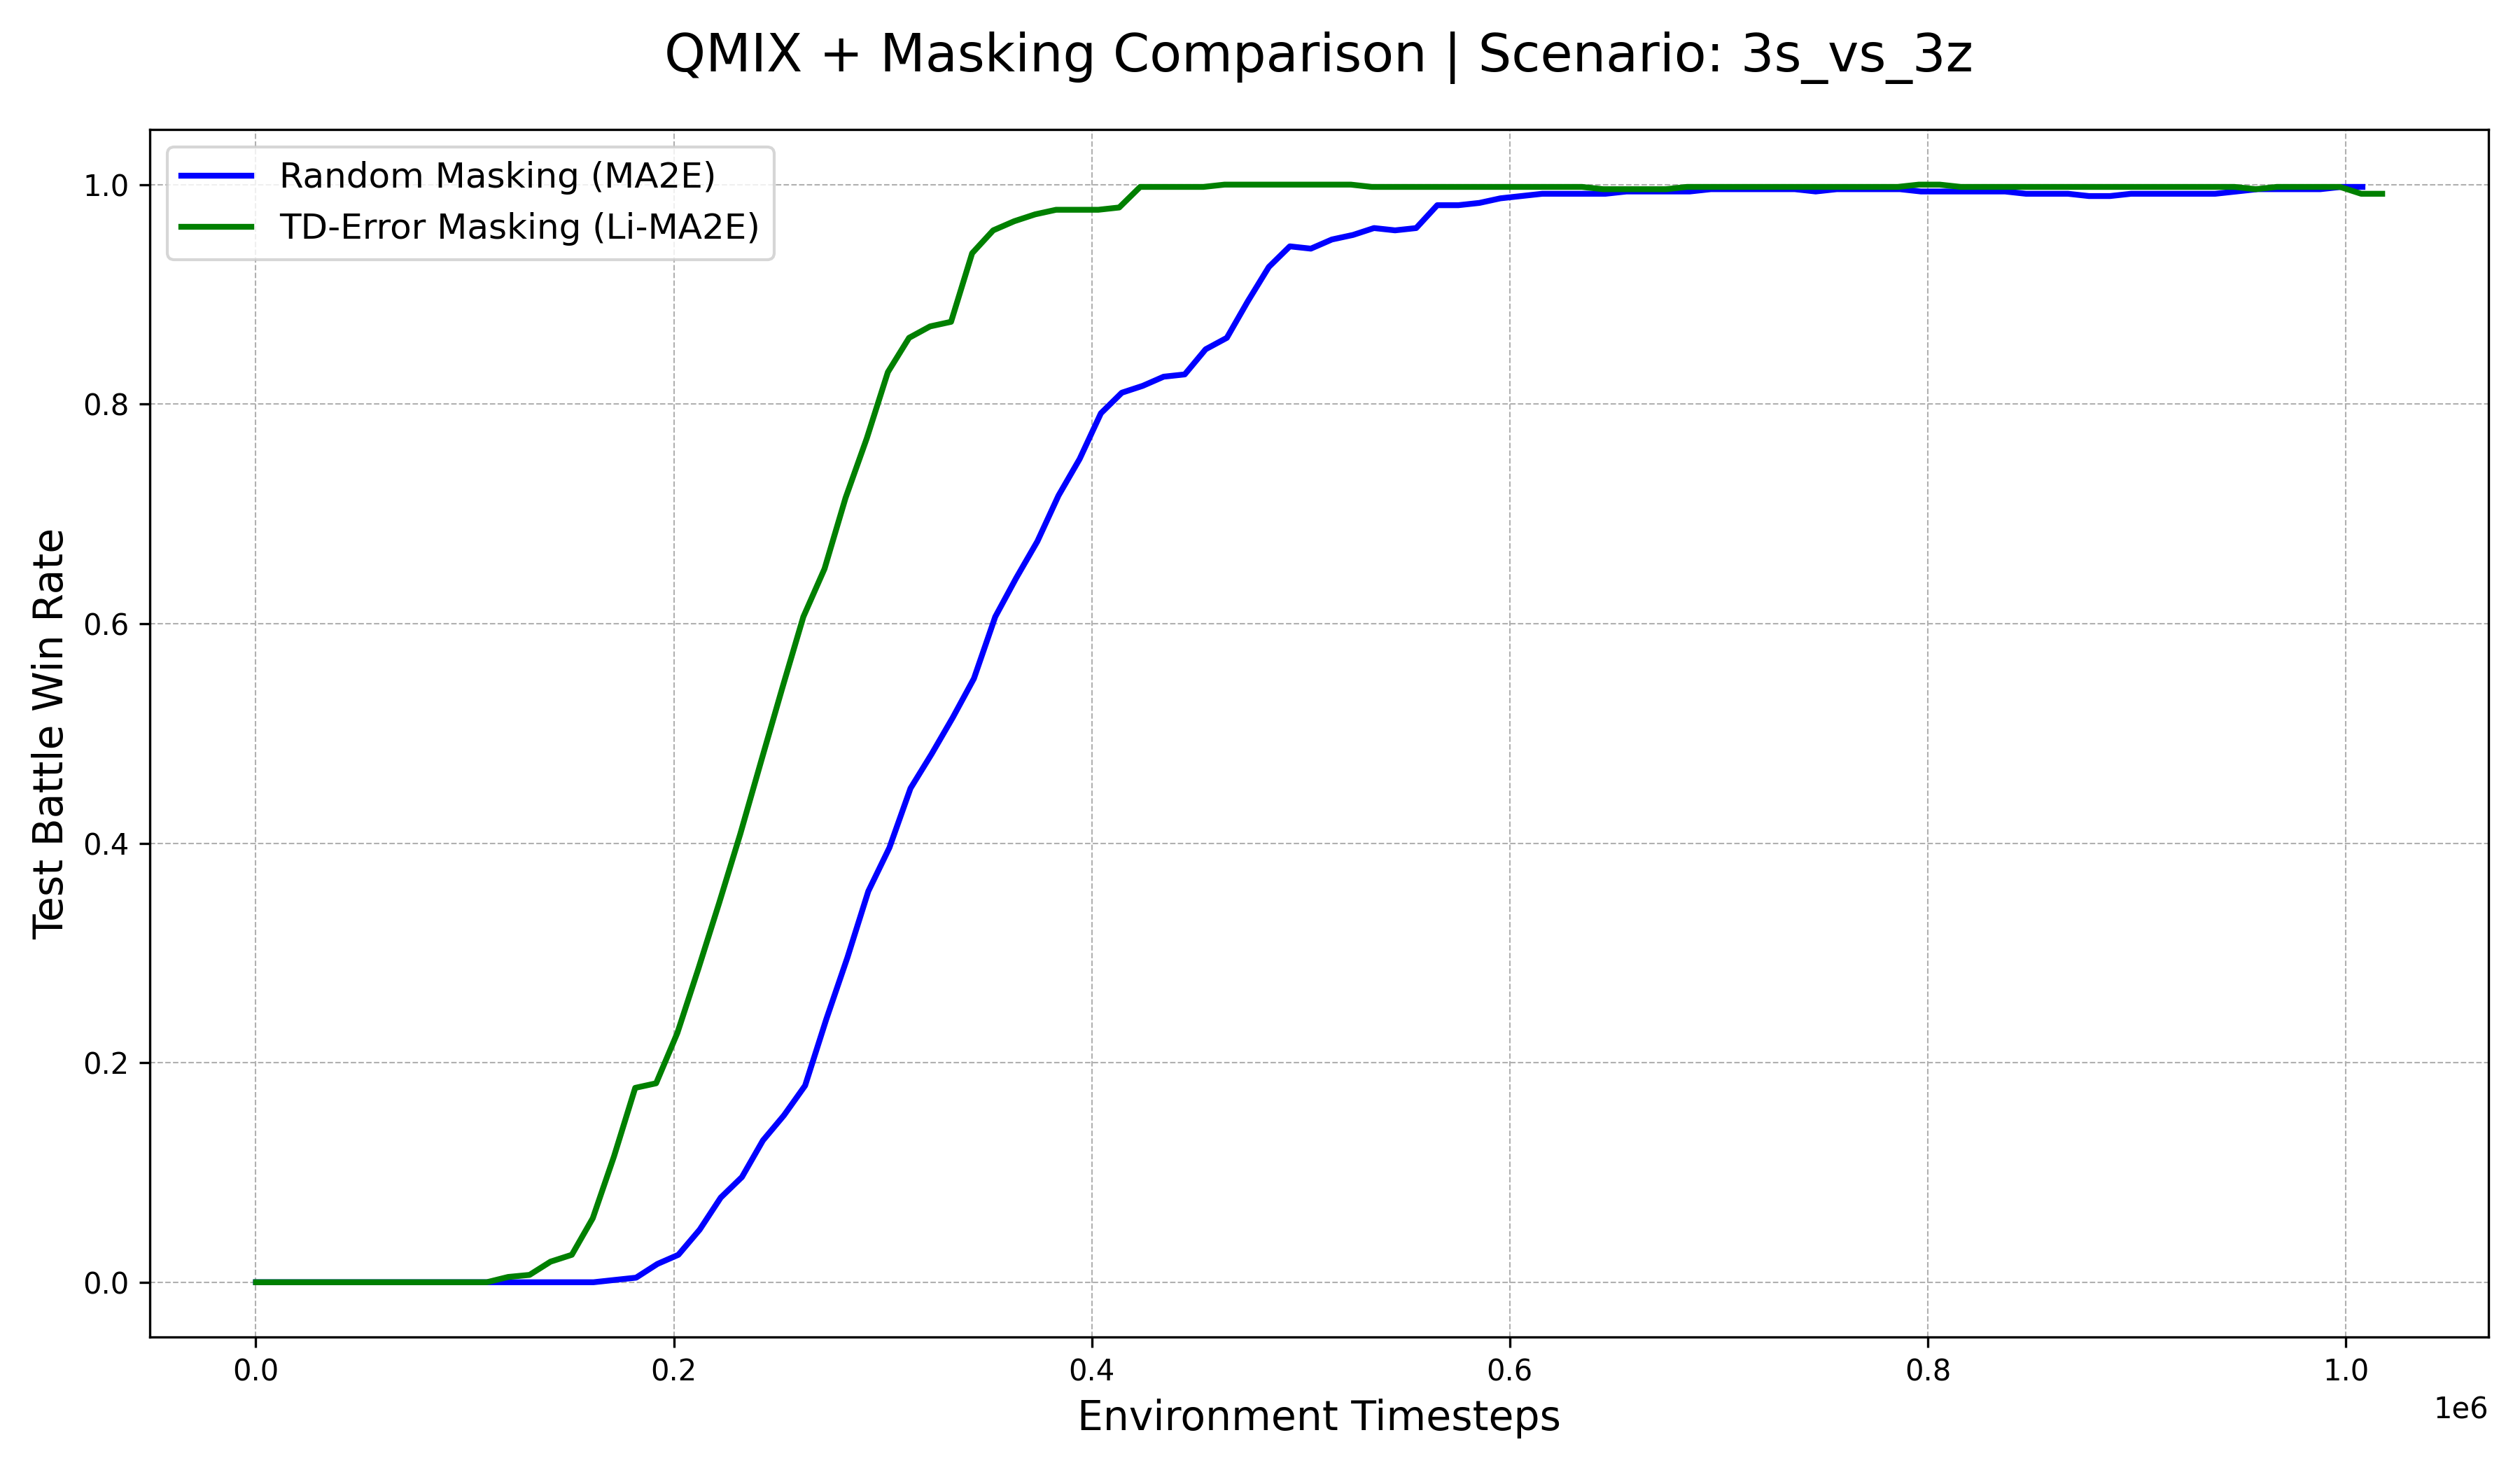
\includegraphics[width=0.8\textwidth]{images_pfe/results_li-ma2e/comparison_plot_3s_vs_3z.png}
    \caption{Performance comparison on the \texttt{3s\_vs\_3z} SMAC map. $LI-{MA}^2E$ demonstrates significantly improved sample efficiency over the baseline.}
    \label{fig:3s_vs_3z}
\end{figure}

\paragraph{Analysis}
In the \texttt{3s\_vs\_3z} scenario, the benefit of our $LI-{MA}^2E$ framework becomes immediately apparent. As shown in Figure~\ref{fig:3s_vs_3z}, the agent guided by TD-Error Masking (green line) learns significantly faster than the baseline agent using Random Masking (blue line).

Our method begins to achieve a non-zero win rate earlier, and its learning curve is considerably steeper, indicating superior sample efficiency. The $LI-{MA}^2E$ agent reaches a perfect win rate at approximately 400,000 timesteps, while the baseline requires around 600,000 timesteps to achieve the same level of performance. This result supports our hypothesis that as scenario complexity increases, an intelligent masking strategy that focuses the MAE's representational power on poorly performing agents provides a distinct advantage, enabling the system to solve the coordination task more rapidly.
\subsubsection{Scenario: \texttt{3s\_vs\_4z}}

Now, we test a harder scenario called \texttt{3s\_vs\_4z}. Here, our \textbf{3 Stalker agents}, who can shoot from a distance, must fight against \textbf{4 enemy Zealot units}, which are durable but can only attack up close.

This test is much more difficult because our agents are \textbf{outnumbered}. To win, they must use two skills together perfectly:
\begin{enumerate}
    \item \textbf{Kiting:} They must keep running away from the Zealots to stay safe, while stopping to shoot them.
    \item \textbf{Focus-Firing:} All three Stalkers must attack the \textit{same} Zealot at the same time to defeat it as quickly as possible.
\end{enumerate}
This requires excellent teamwork to succeed. The results of this difficult test are shown in Figure~\ref{fig:3s_vs_4z}.

\begin{figure}[h]
    \centering
     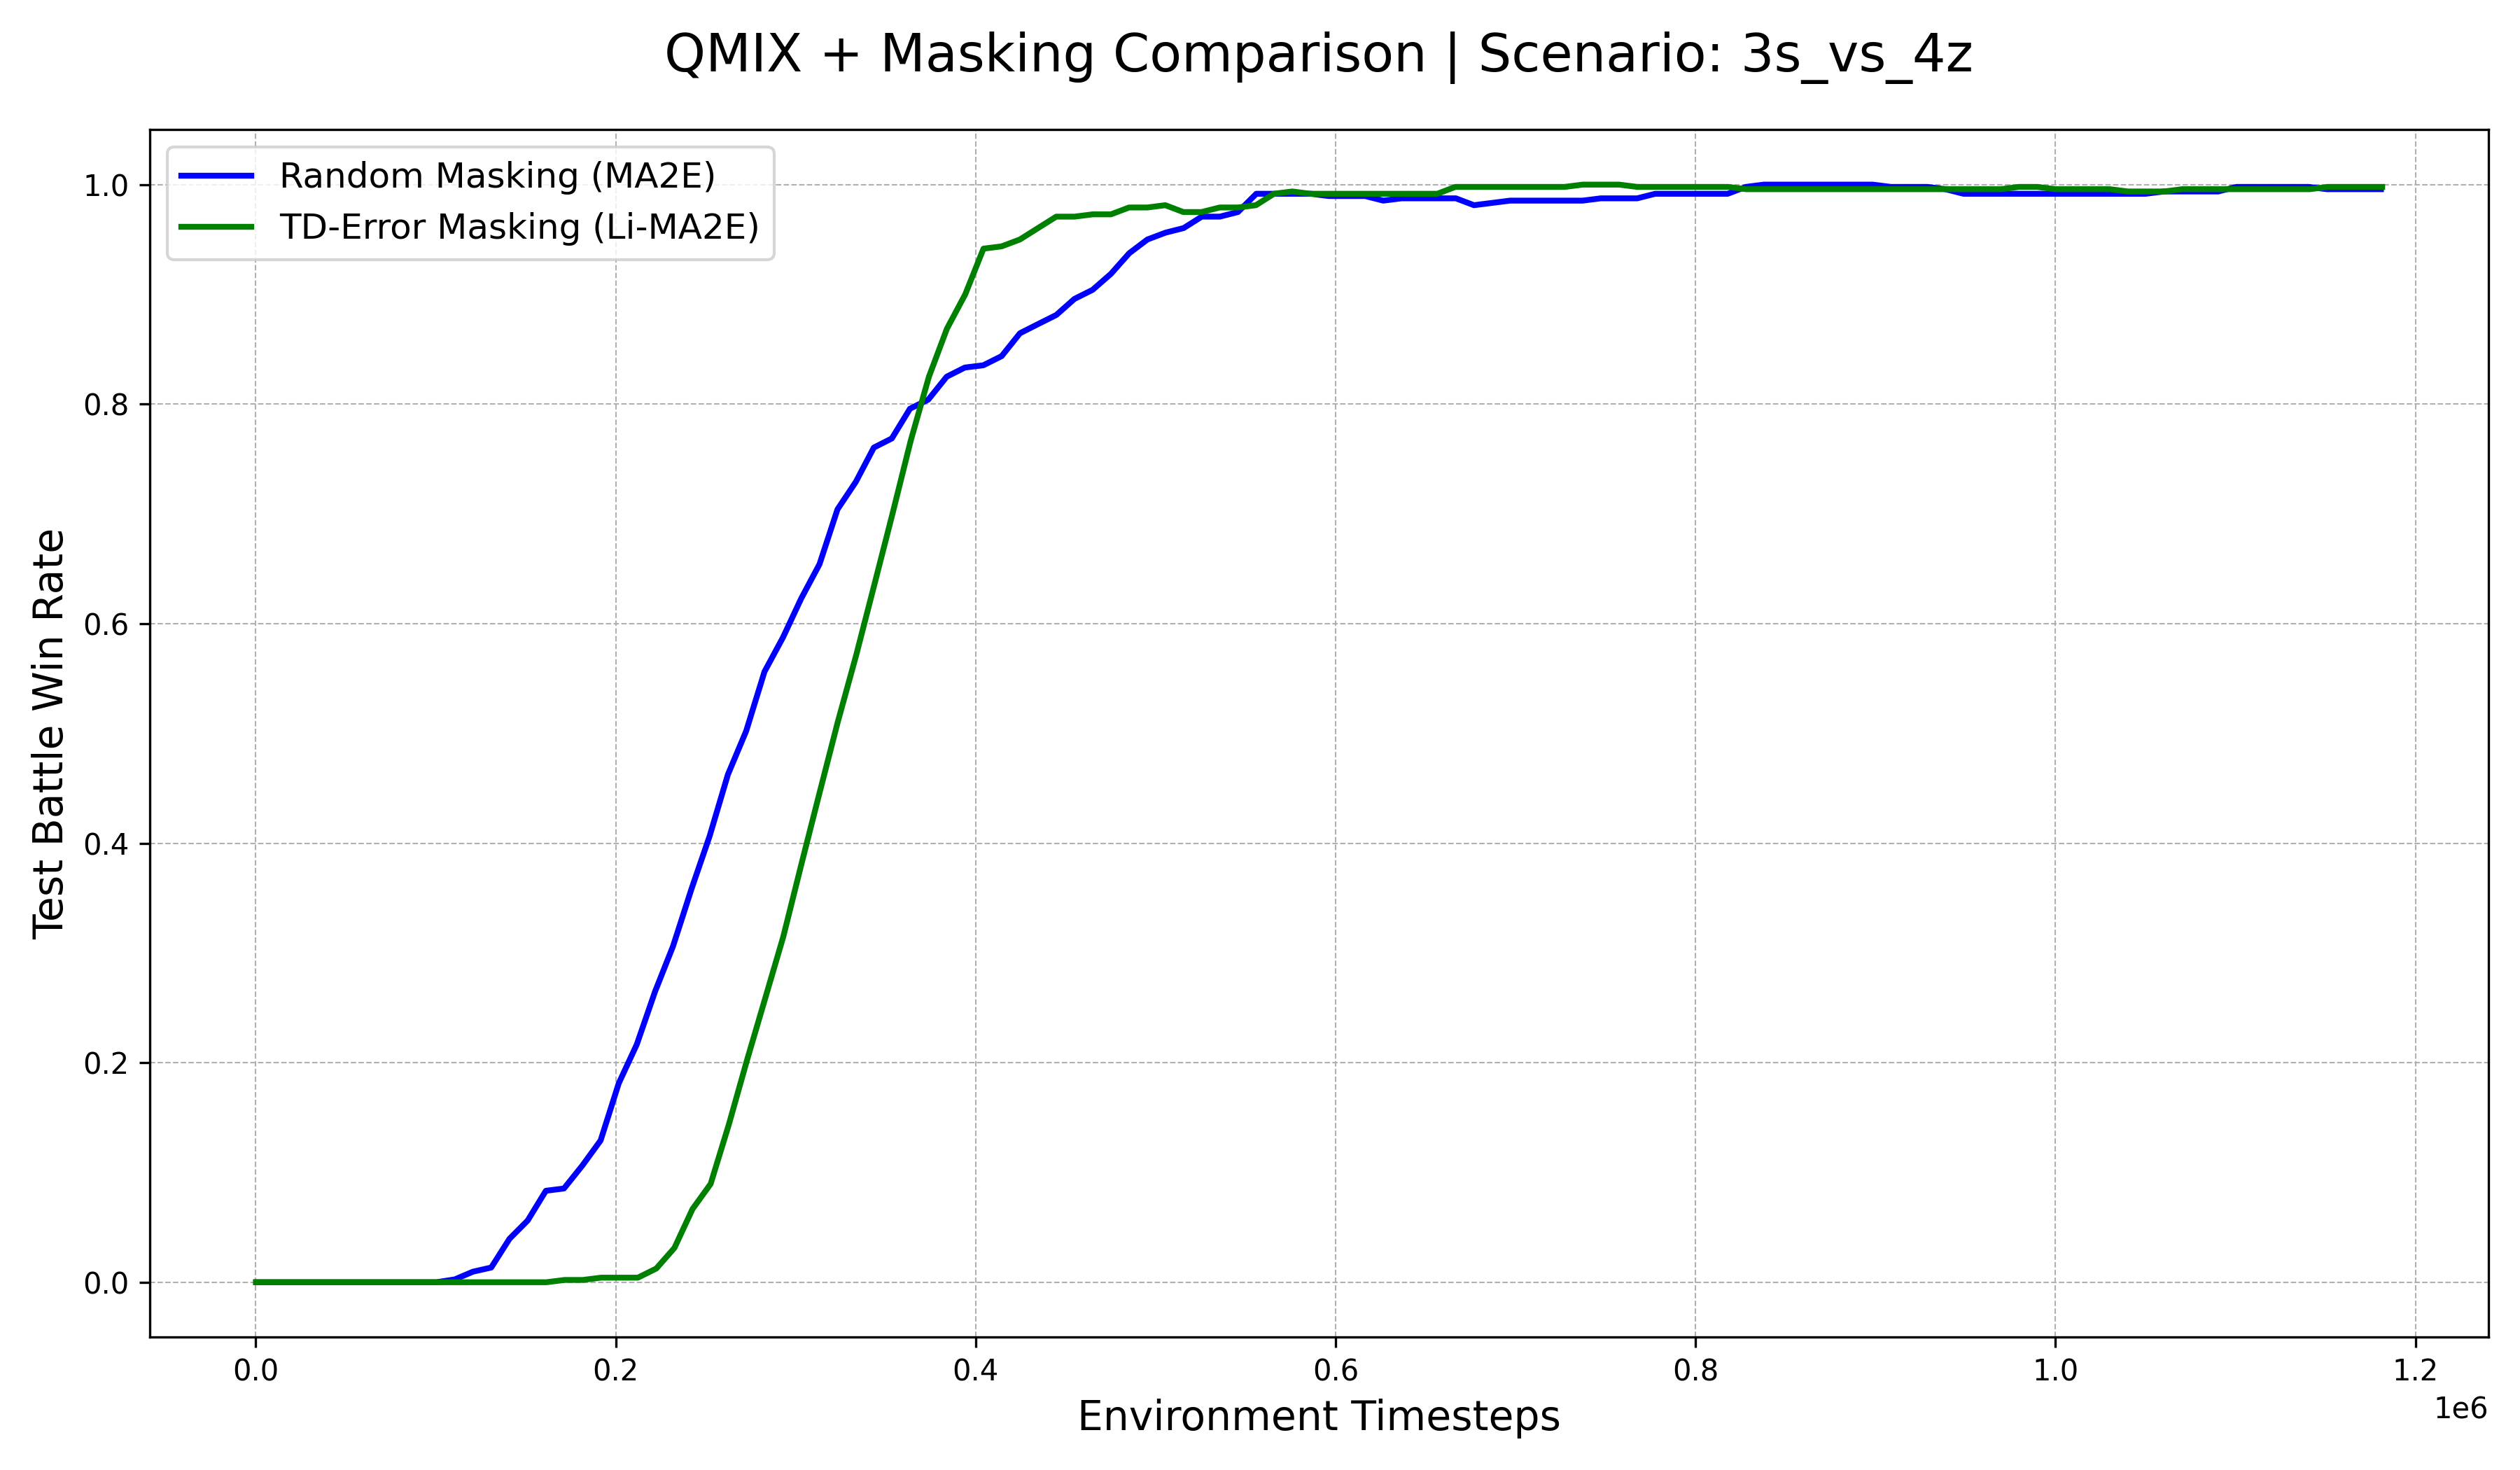
\includegraphics[width=0.8\textwidth]{images_pfe/results_li-ma2e/comparison_plot_3s_vs_4z.png}
    \caption{Performance comparison on the \texttt{3s\_vs\_4z} SMAC map. The plot shows a trade-off between the faster initial learning of the baseline and the more stable final convergence of $LI-{MA}^2E$.}
    \label{fig:3s_vs_4z}
\end{figure}

\paragraph{Analysis}
The \texttt{3s\_vs\_4z} scenario reveals an interesting trade-off between learning speed and final policy stability. As shown in Figure~\ref{fig:3s_vs_4z}, the baseline ${MA}^2E$ with Random Masking (blue line) exhibits a faster initial learning curve, reaching a high win rate more quickly.

However, a closer look at the convergence phase (after 0.6 million timesteps) shows that our $LI-{MA}^2E$ framework (green line) achieves a more stable and decisive convergence at a 100\% win rate. The baseline's performance, in contrast, shows more fluctuation before finally settling. This suggests that while the exploratory nature of random masking may find a working solution faster in this specific scenario, the guided approach of $LI-{MA}^2E$ produces a more robust and stable final policy.


\subsubsection{Scenario: \texttt{3s\_vs\_5z}}

Next, we test our method on \texttt{3s\_vs\_5z}, a very hard challenge from the \texttt{HARD} difficulty category. In this test, our \textbf{3 Stalker agents} (who shoot from a distance) are heavily outnumbered by \textbf{5 durable enemy Zealots} (who attack up close).

To win this difficult fight, the agents must be perfect at two skills at the same time:
\begin{enumerate}
    \item \textbf{Kiting:} They must always keep running away from the Zealots to avoid taking damage, while still turning to shoot.
    \item \textbf{Focus-Firing:} All three of our agents must attack the exact same enemy at the same time. This is the only way to defeat one of the five enemies quickly.
\end{enumerate}
This is a major test of teamwork. If even one agent makes a mistake, the team will likely lose. The agents must learn to coordinate perfectly to survive and win. The results for this difficult test are shown in Figure~\ref{fig:3s_vs_5z}.

\begin{figure}[h]
    \centering
    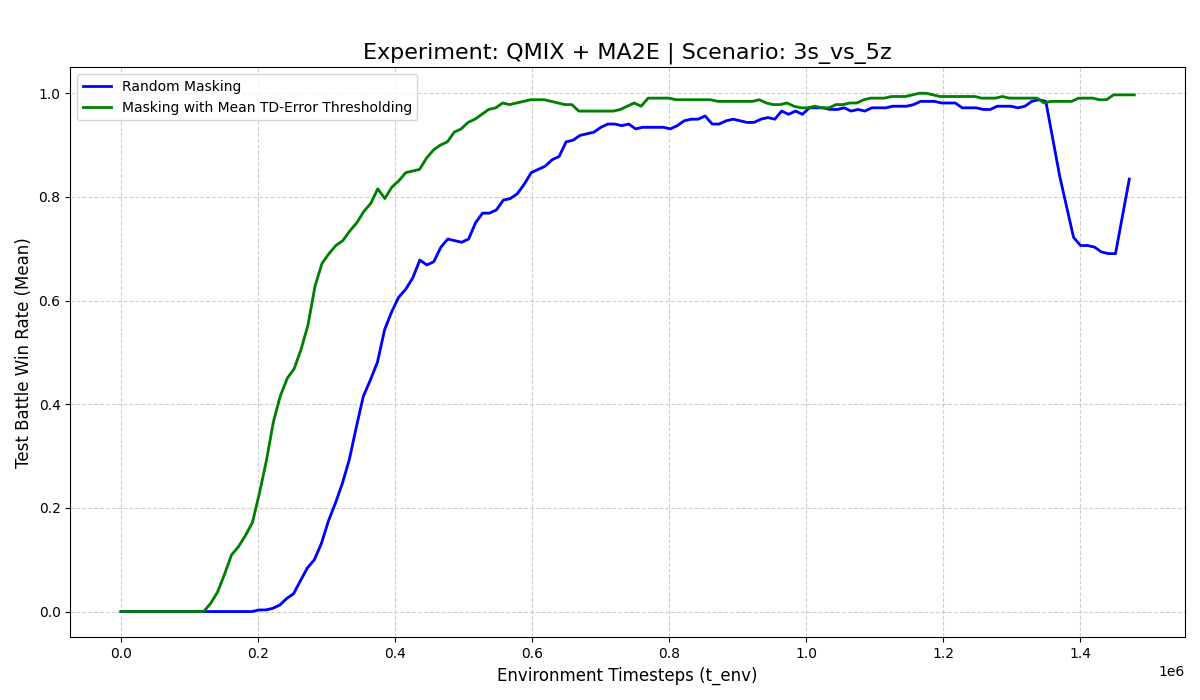
\includegraphics[width=0.8\textwidth]{images_pfe/results_li-ma2e/test_battle_won_mean_3s_vs_5z_Mean_TD-Error_Thresholding _smoothed.png}
    \caption{Performance comparison on the \texttt{3s\_vs\_5z} HARD scenario. In this complex asymmetric task, $LI-{MA}^2E$ demonstrates vastly superior sample efficiency and produces a more stable final policy compared to the baseline Random Masking.}
    \label{fig:3s_vs_5z}
\end{figure}

\paragraph{Analysis}
In stark contrast to the previous map, the results on \texttt{3s\_vs\_5z} show a clear and significant advantage for our $LI-{MA}^2E$ framework (green line). The intelligent masking strategy leads to a dramatic improvement in both sample efficiency and final policy stability.

$LI-{MA}^2E$ learns much faster, achieving a near-perfect win rate before 0.6 million timesteps, while the baseline with random masking (blue line) requires more than 1.2 million timesteps to reach a similar peak performance. Crucially, during the later stages of training (after 1.3 million steps), the baseline policy exhibits significant instability with a sharp drop in performance, a behavior not observed in our method.

This strong result supports our core hypothesis. The \texttt{3s\_vs\_5z} map requires precise, coordinated kiting, where a single agent's mistake can be catastrophic. By adaptively focusing the MAE's reconstruction on the agent with the highest immediate error, our framework helps the team learn this essential cooperative strategy more effectively and robustly. The final stability of the $LI-{MA}^2E$ policy suggests that it has discovered a more general and resilient solution compared to the brittle policy learned by the baseline.

\subsubsection{Scenario: \texttt{8m}}
We continue our evaluation with the \texttt{8m} scenario, a symmetric map which pits \textbf{8 allied Marines against eight enemy Marines}. This task increases the number of homogeneous agents compared to \texttt{3m} and demands effective \textbf{focus-firing} to succeed. Focus-firing is a critical coordination strategy where multiple agents target and eliminate a single enemy unit at a time. This tactic maximizes the applied damage and removes sources of enemy fire from the battlefield as quickly as possible, representing a significant coordination challenge for a multi-agent system. The results are presented in Figure~\ref{fig:8m}.

\begin{figure}[h]
    \centering
    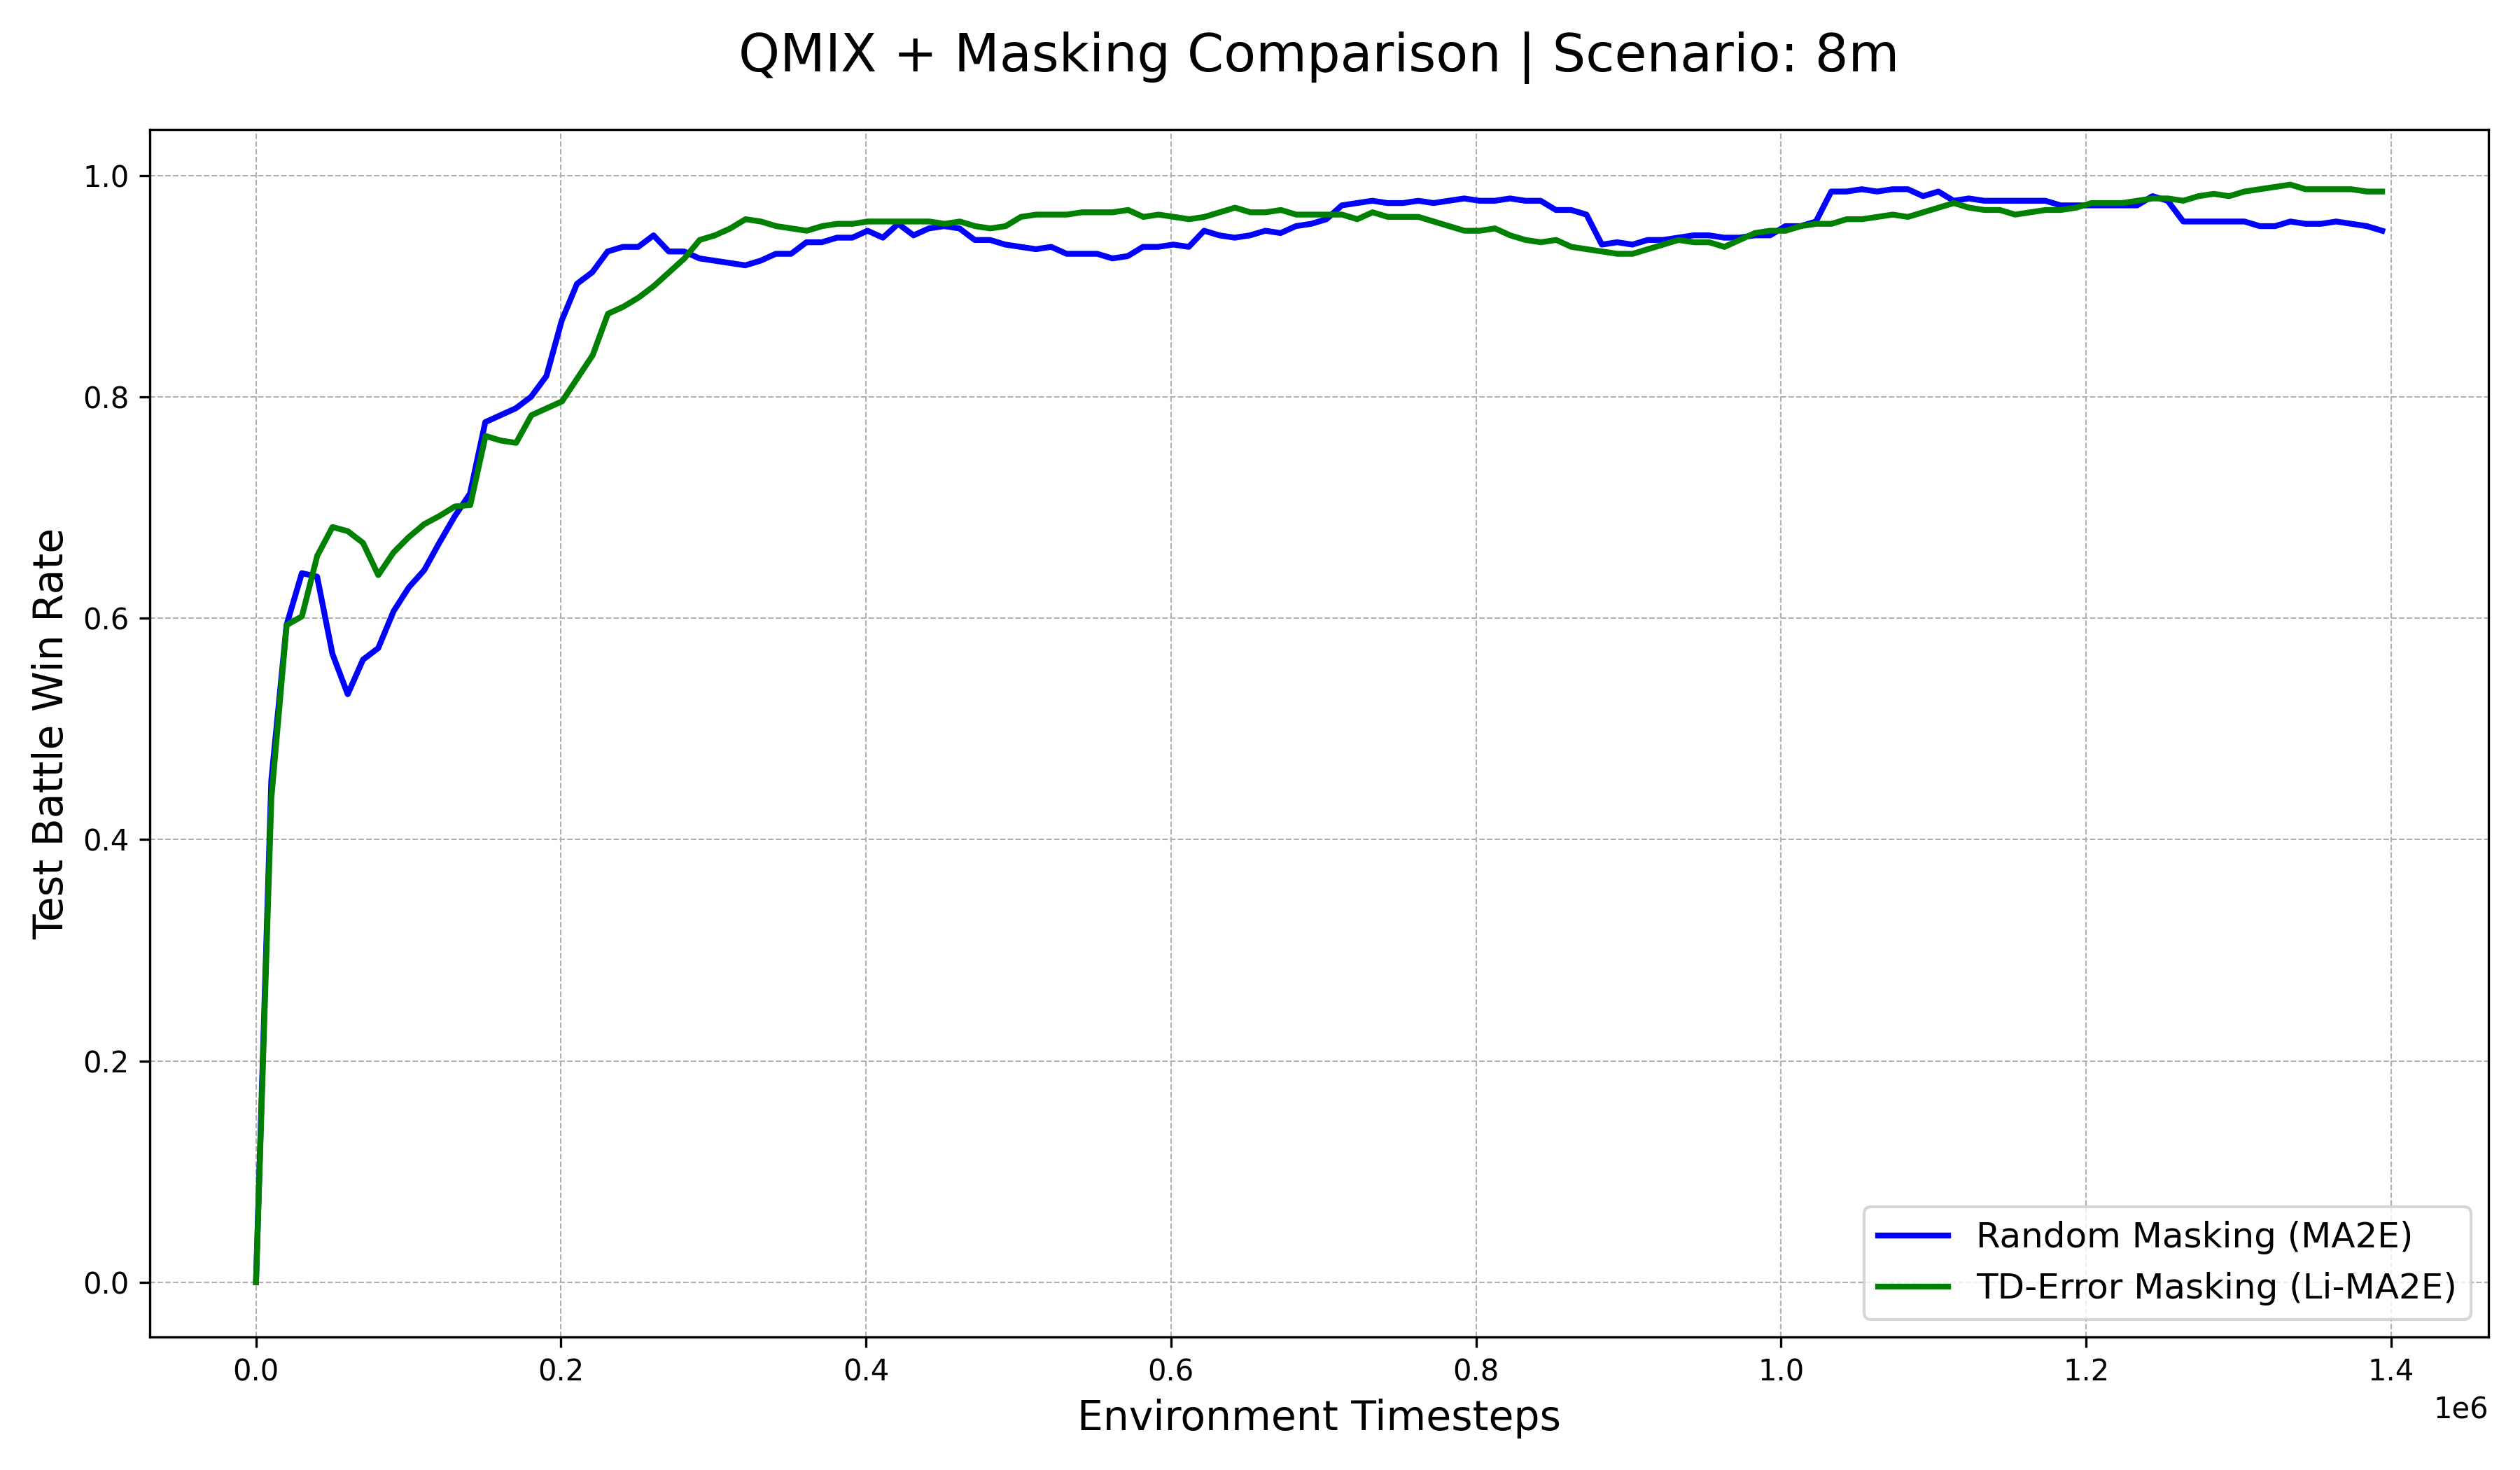
\includegraphics[width=0.8\textwidth]{images_pfe/results_li-ma2e/comparison_plot_8m.png}
    \caption{Performance comparison on the \texttt{8m} SMAC map. Both methods converge to a perfect win rate, with the baseline showing a faster initial learning rate.}
    \label{fig:8m}
\end{figure}
\paragraph{Analysis}
Upon careful re-examination of the provided plot for the \texttt{8m} scenario, the results show a nuanced competition between the two methods. The baseline Random Masking (blue line) demonstrates a higher sample efficiency during the initial critical learning phase.

As seen in Figure~\ref{fig:8m}, the blue line's win rate rises more steeply and consistently between 0.1 million and 0.3 million timesteps, reaching a high level of performance first. The $LI-{MA}^2E$ method (green line), while also learning the task, shows a noticeable dip in performance around 0.15 million timesteps and follows a slower learning trajectory in this initial phase. Both methods do eventually converge to a near-perfect win rate after approximately 1.0 million timesteps, showing that both can ultimately solve this scenario. However, the advantage in learning speed in this case belongs to the baseline.

This finding suggests that in this specific homogeneous scenario with a larger number of agents, the broader, exploratory nature of random masking may be more effective at building a general representation than the more focused TD-error approach. This helps to define the conditions under which our $LI-{MA}^2E$ provides the most significant advantage, namely, in more complex, asymmetric scenarios.


\paragraph{Answer to RQ1:}
In summary, the evidence shows that the answer to this question is \textbf{yes, particularly in complex, asymmetric scenarios.} While the performance of $LI-{MA}^2E$ is comparable on simple maps, it demonstrates significantly improved sample efficiency and final policy stability on complex maps like \texttt{3s\_vs\_5z}. This suggests that our method yields more reliable task completion when coordination is most critical.

%----------------------------------------------------------------------------------------
\subsection{RQ2: Does Our Masking Lead to Higher-Quality Policies?}
%----------------------------------------------------------------------------------------

Beyond simply winning, a superior algorithm should learn to win more efficiently. To investigate this, we analyze the \textbf{mean test return}. This metric reflects the \textit{quality} and \textit{efficiency} of the learned policy, where a higher return often corresponds to winning with more surviving units or in less time.


\begin{figure}[h]
    \centering
    % Row 1 of plots
    \subfloat[Scenario: 3m]{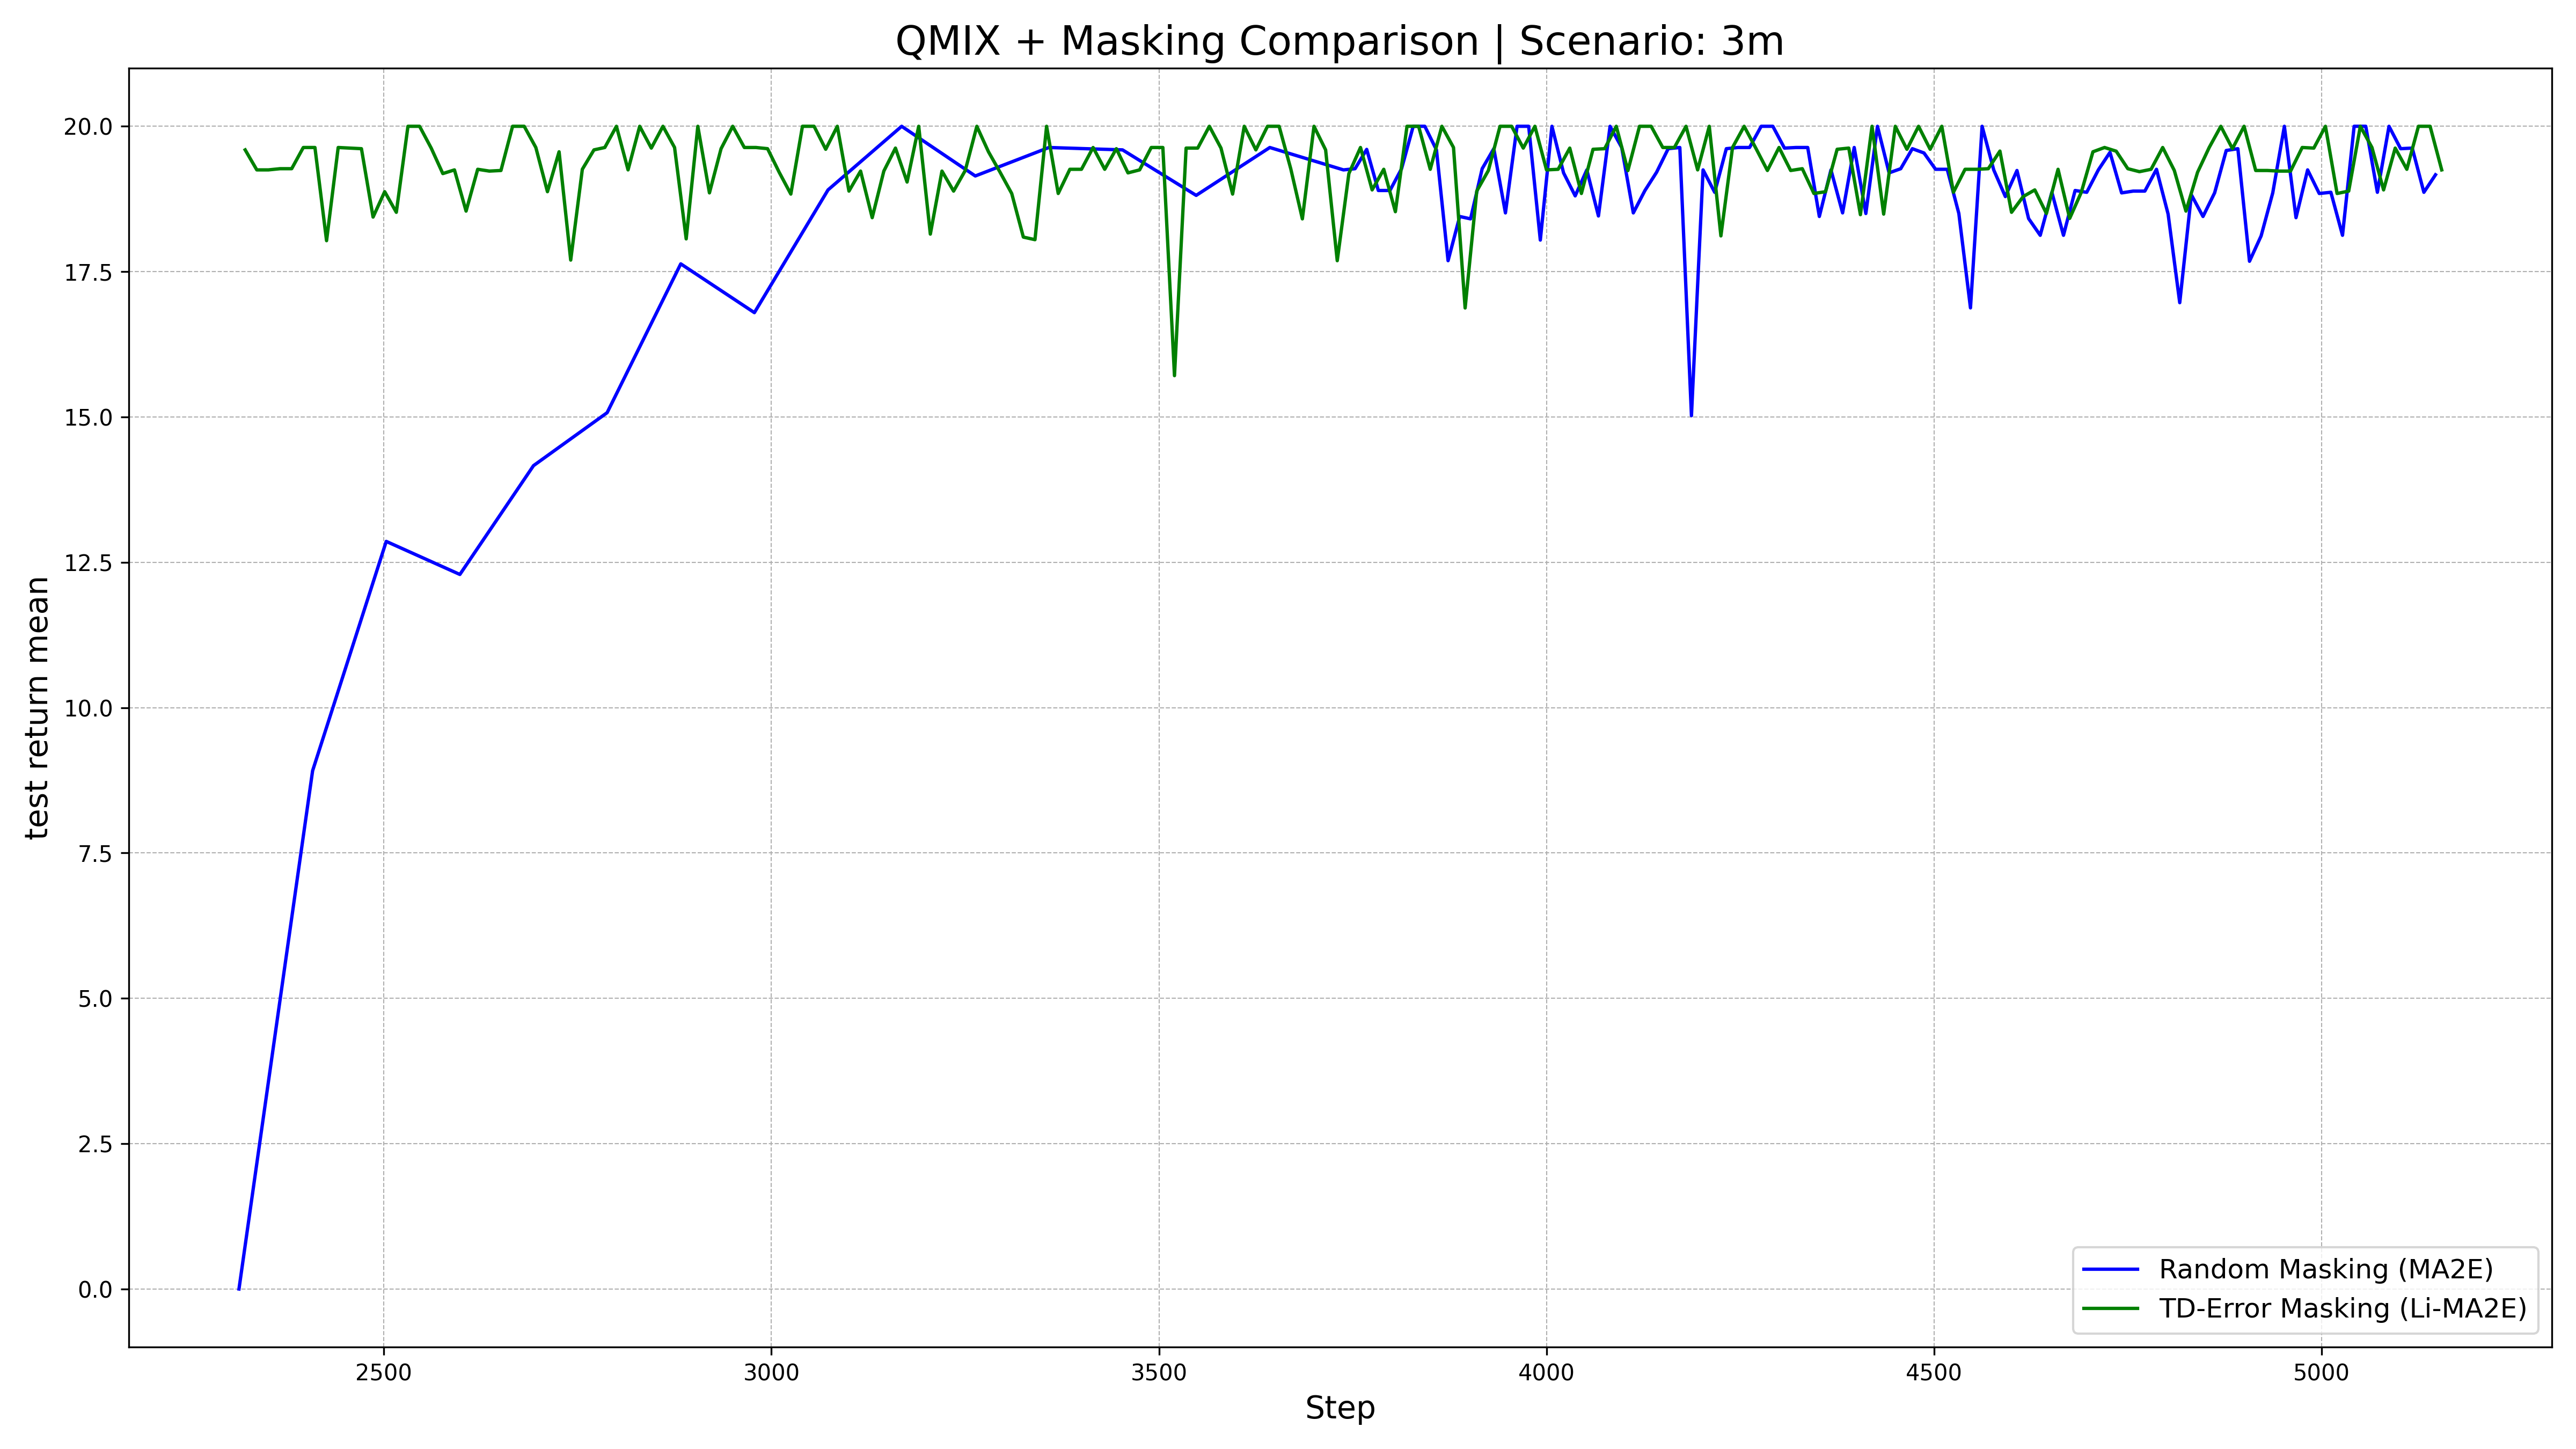
\includegraphics[width=0.32\textwidth]{images_pfe/results_test_return_mean/comparison_plot_3m.png}
    \label{fig:3m_return}}
    \hfill
    \subfloat[Scenario: 3s\_vs\_3z]{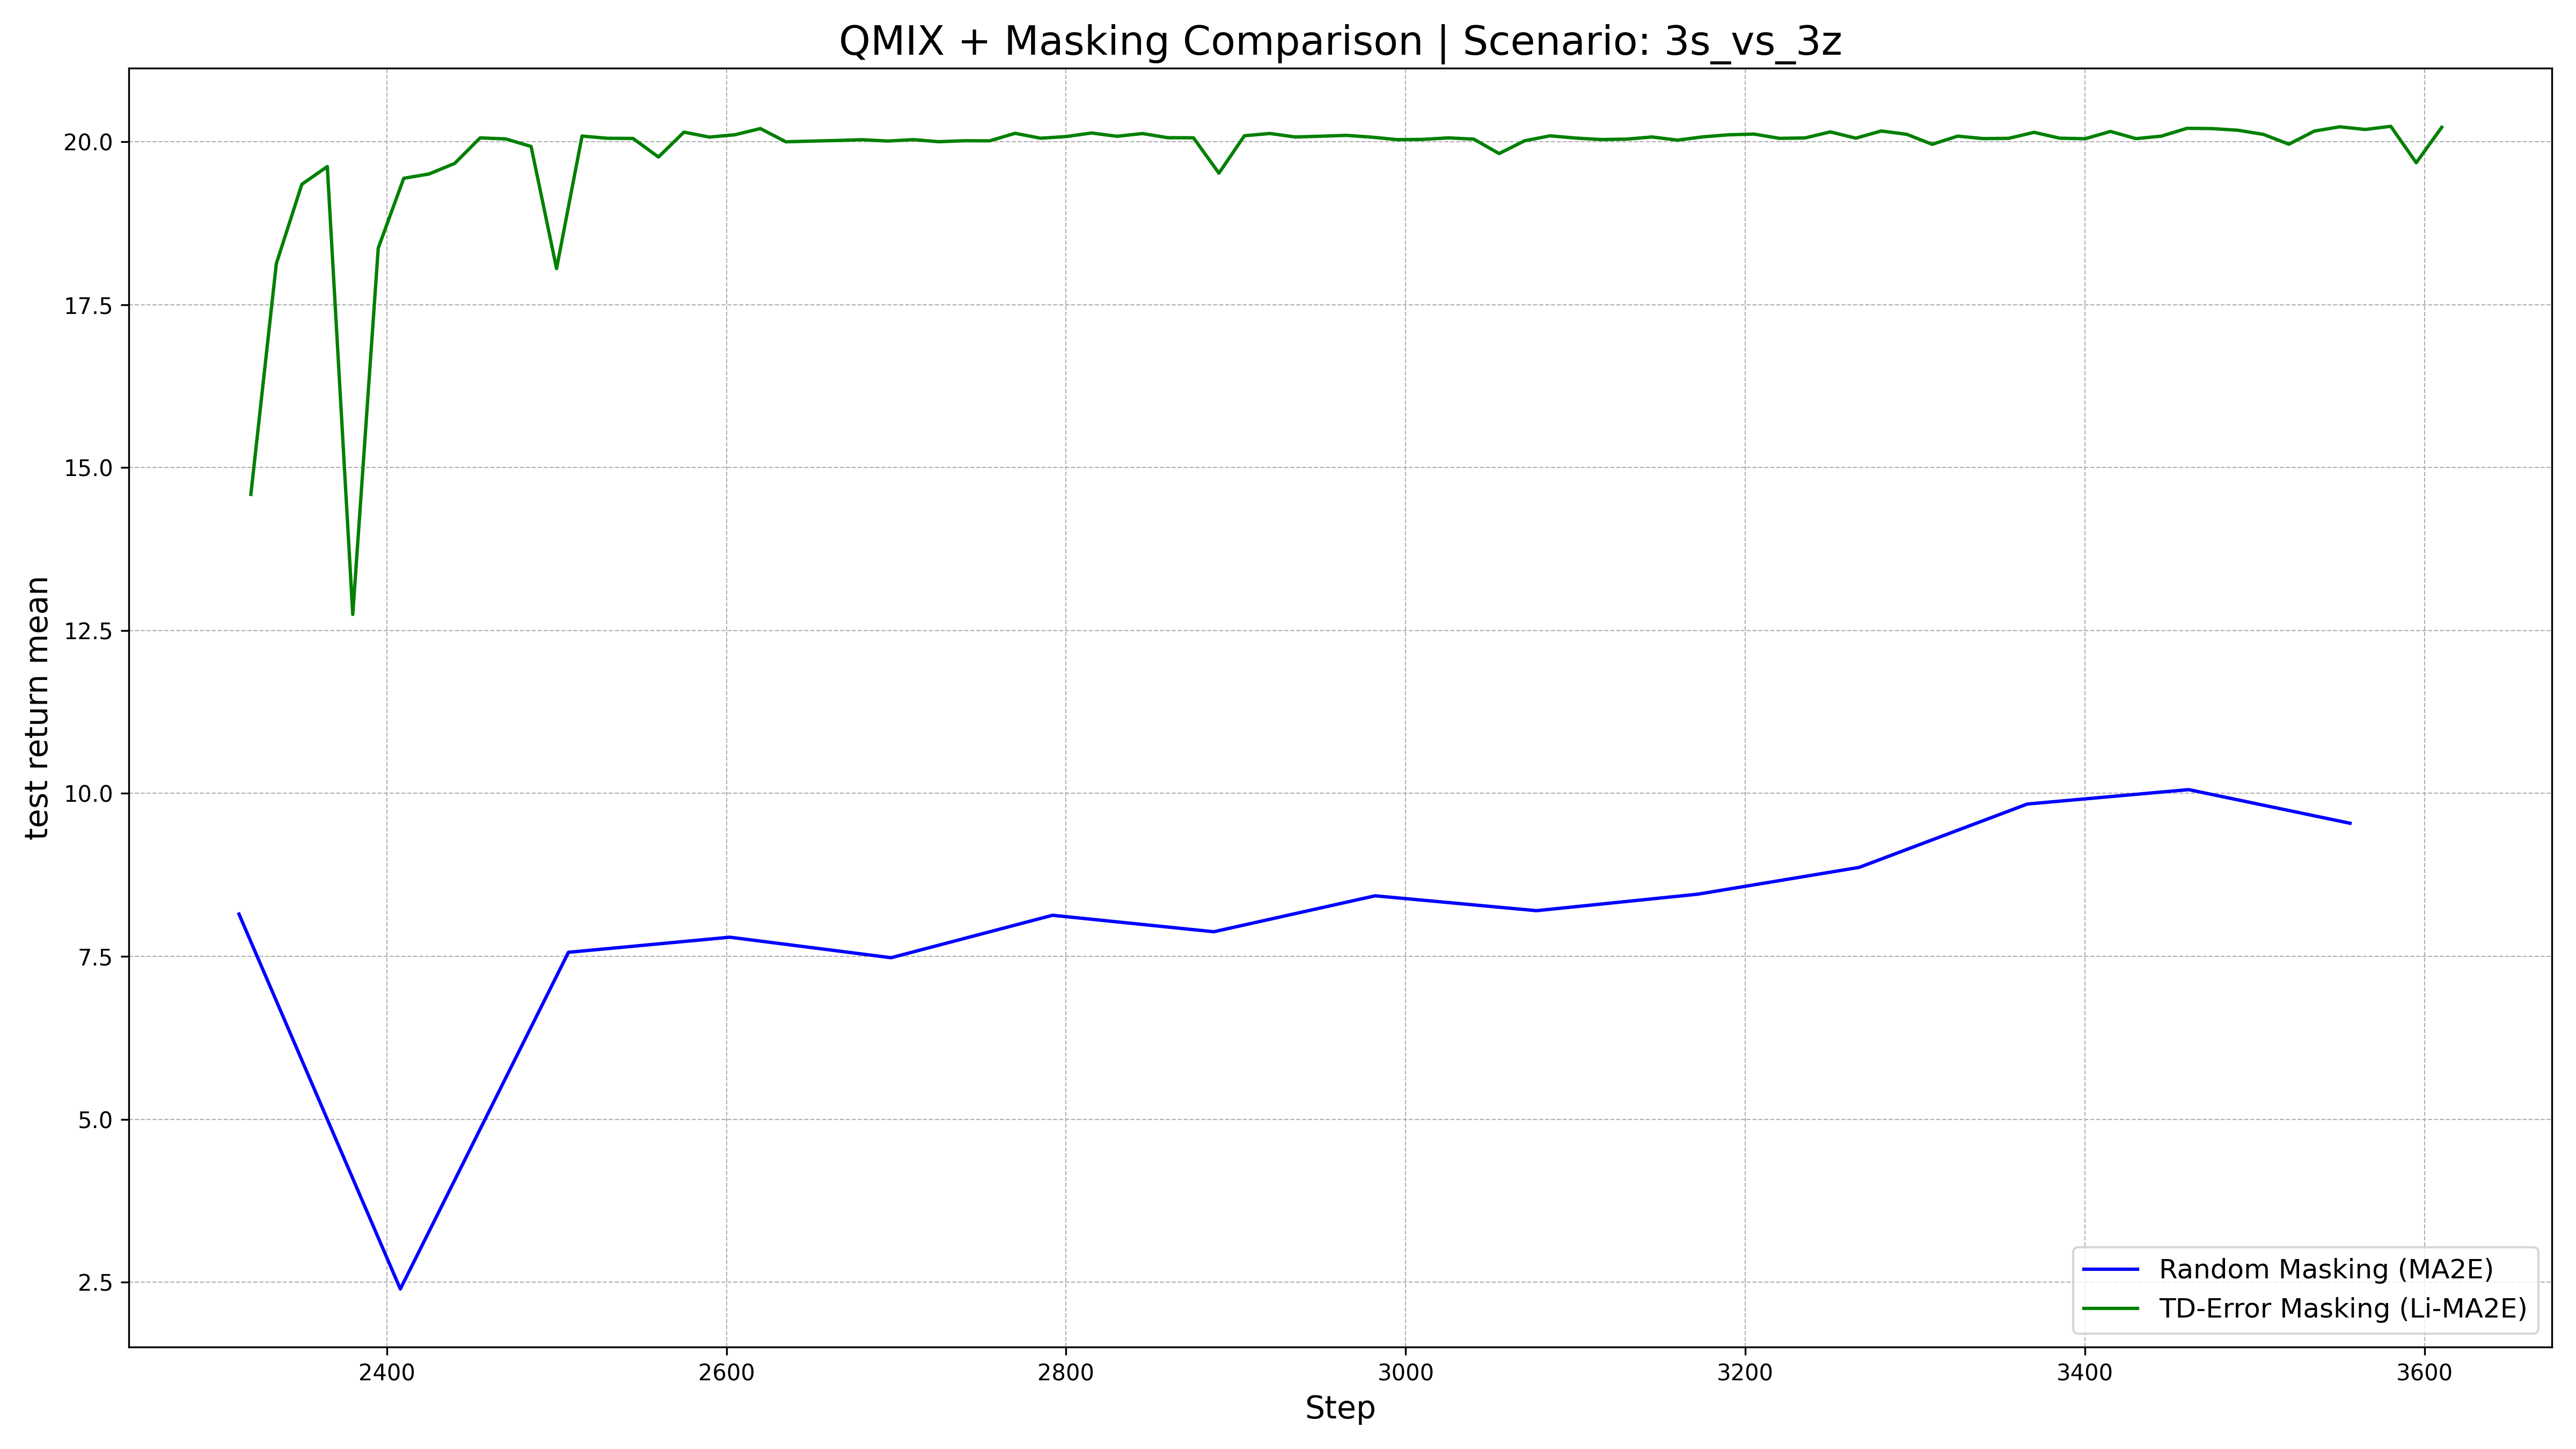
\includegraphics[width=0.32\textwidth]{images_pfe/results_test_return_mean/comparison_plot_3s_vs_3z.png}
    \label{fig:3s_vs_3z_return}}
    \hfill
    \subfloat[Scenario: 3s\_vs\_4z]{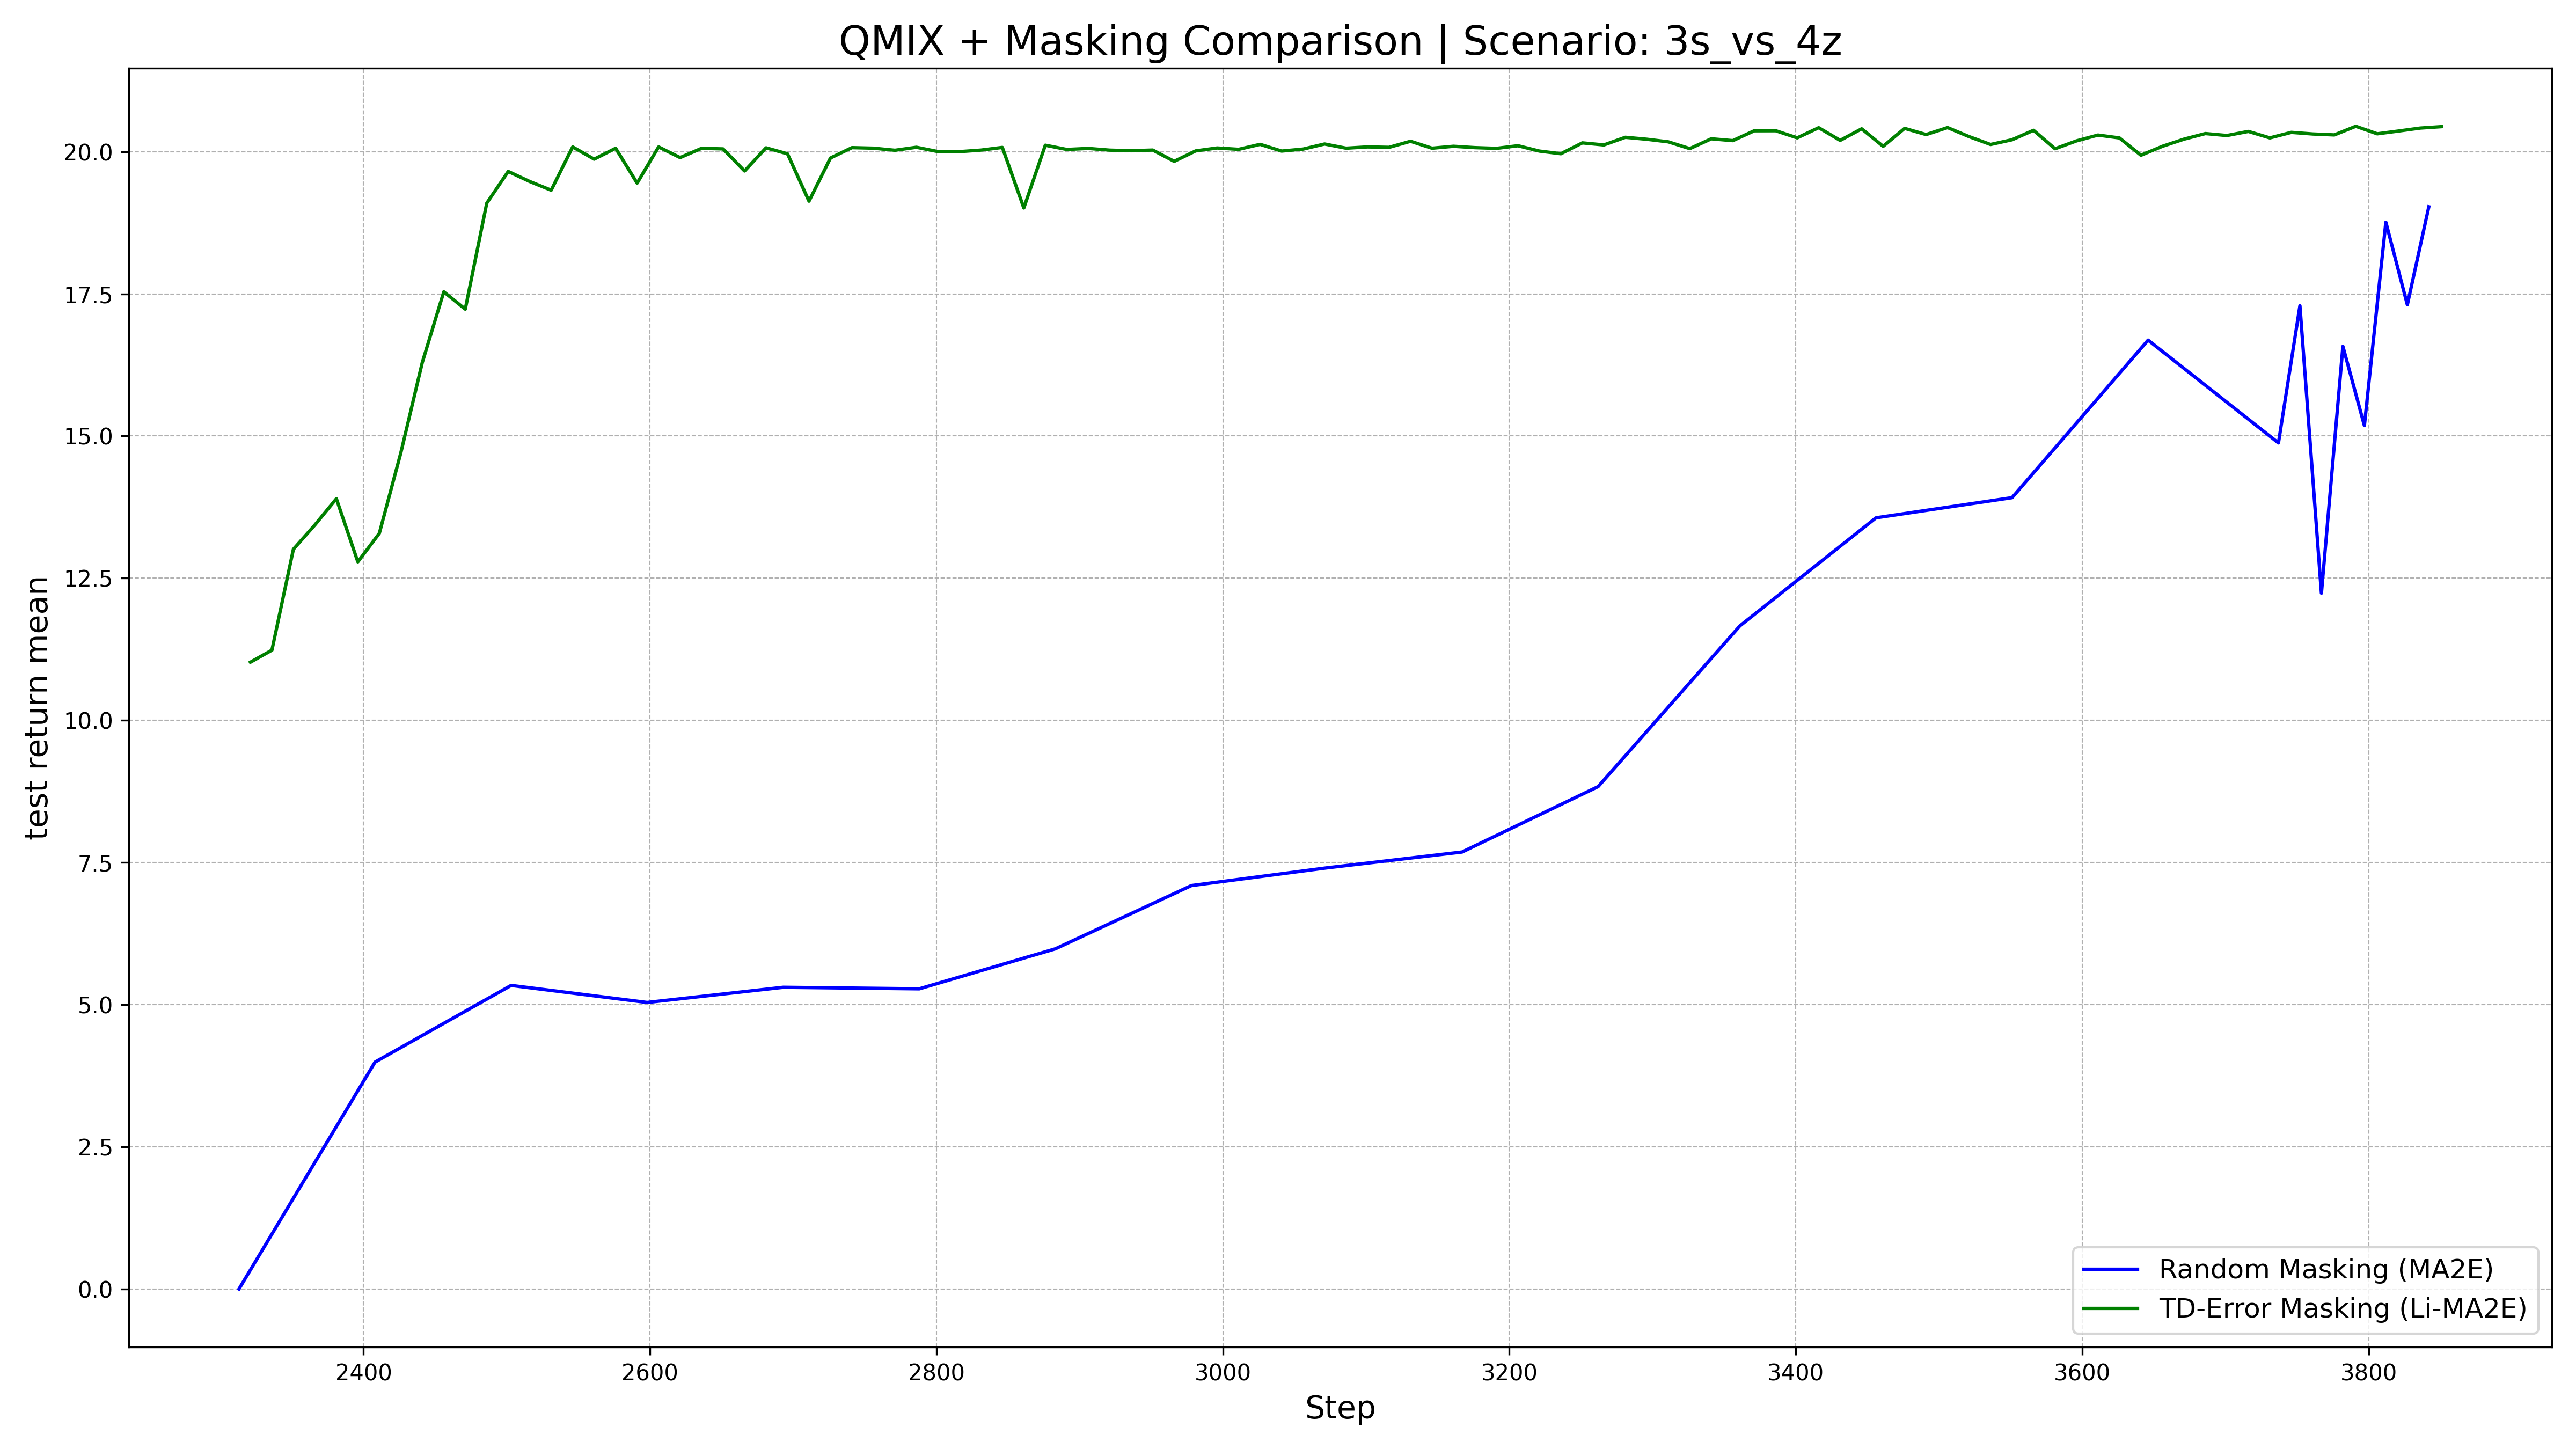
\includegraphics[width=0.32\textwidth]{images_pfe/results_test_return_mean/comparison_plot_3s_vs_4z.png}\label{fig:3s_vs_4z_return}}
    
    \vspace{1em} % Adds a little vertical space between rows
    
    % Row 2 of plots
    \subfloat[Scenario: 3s\_vs\_5z]{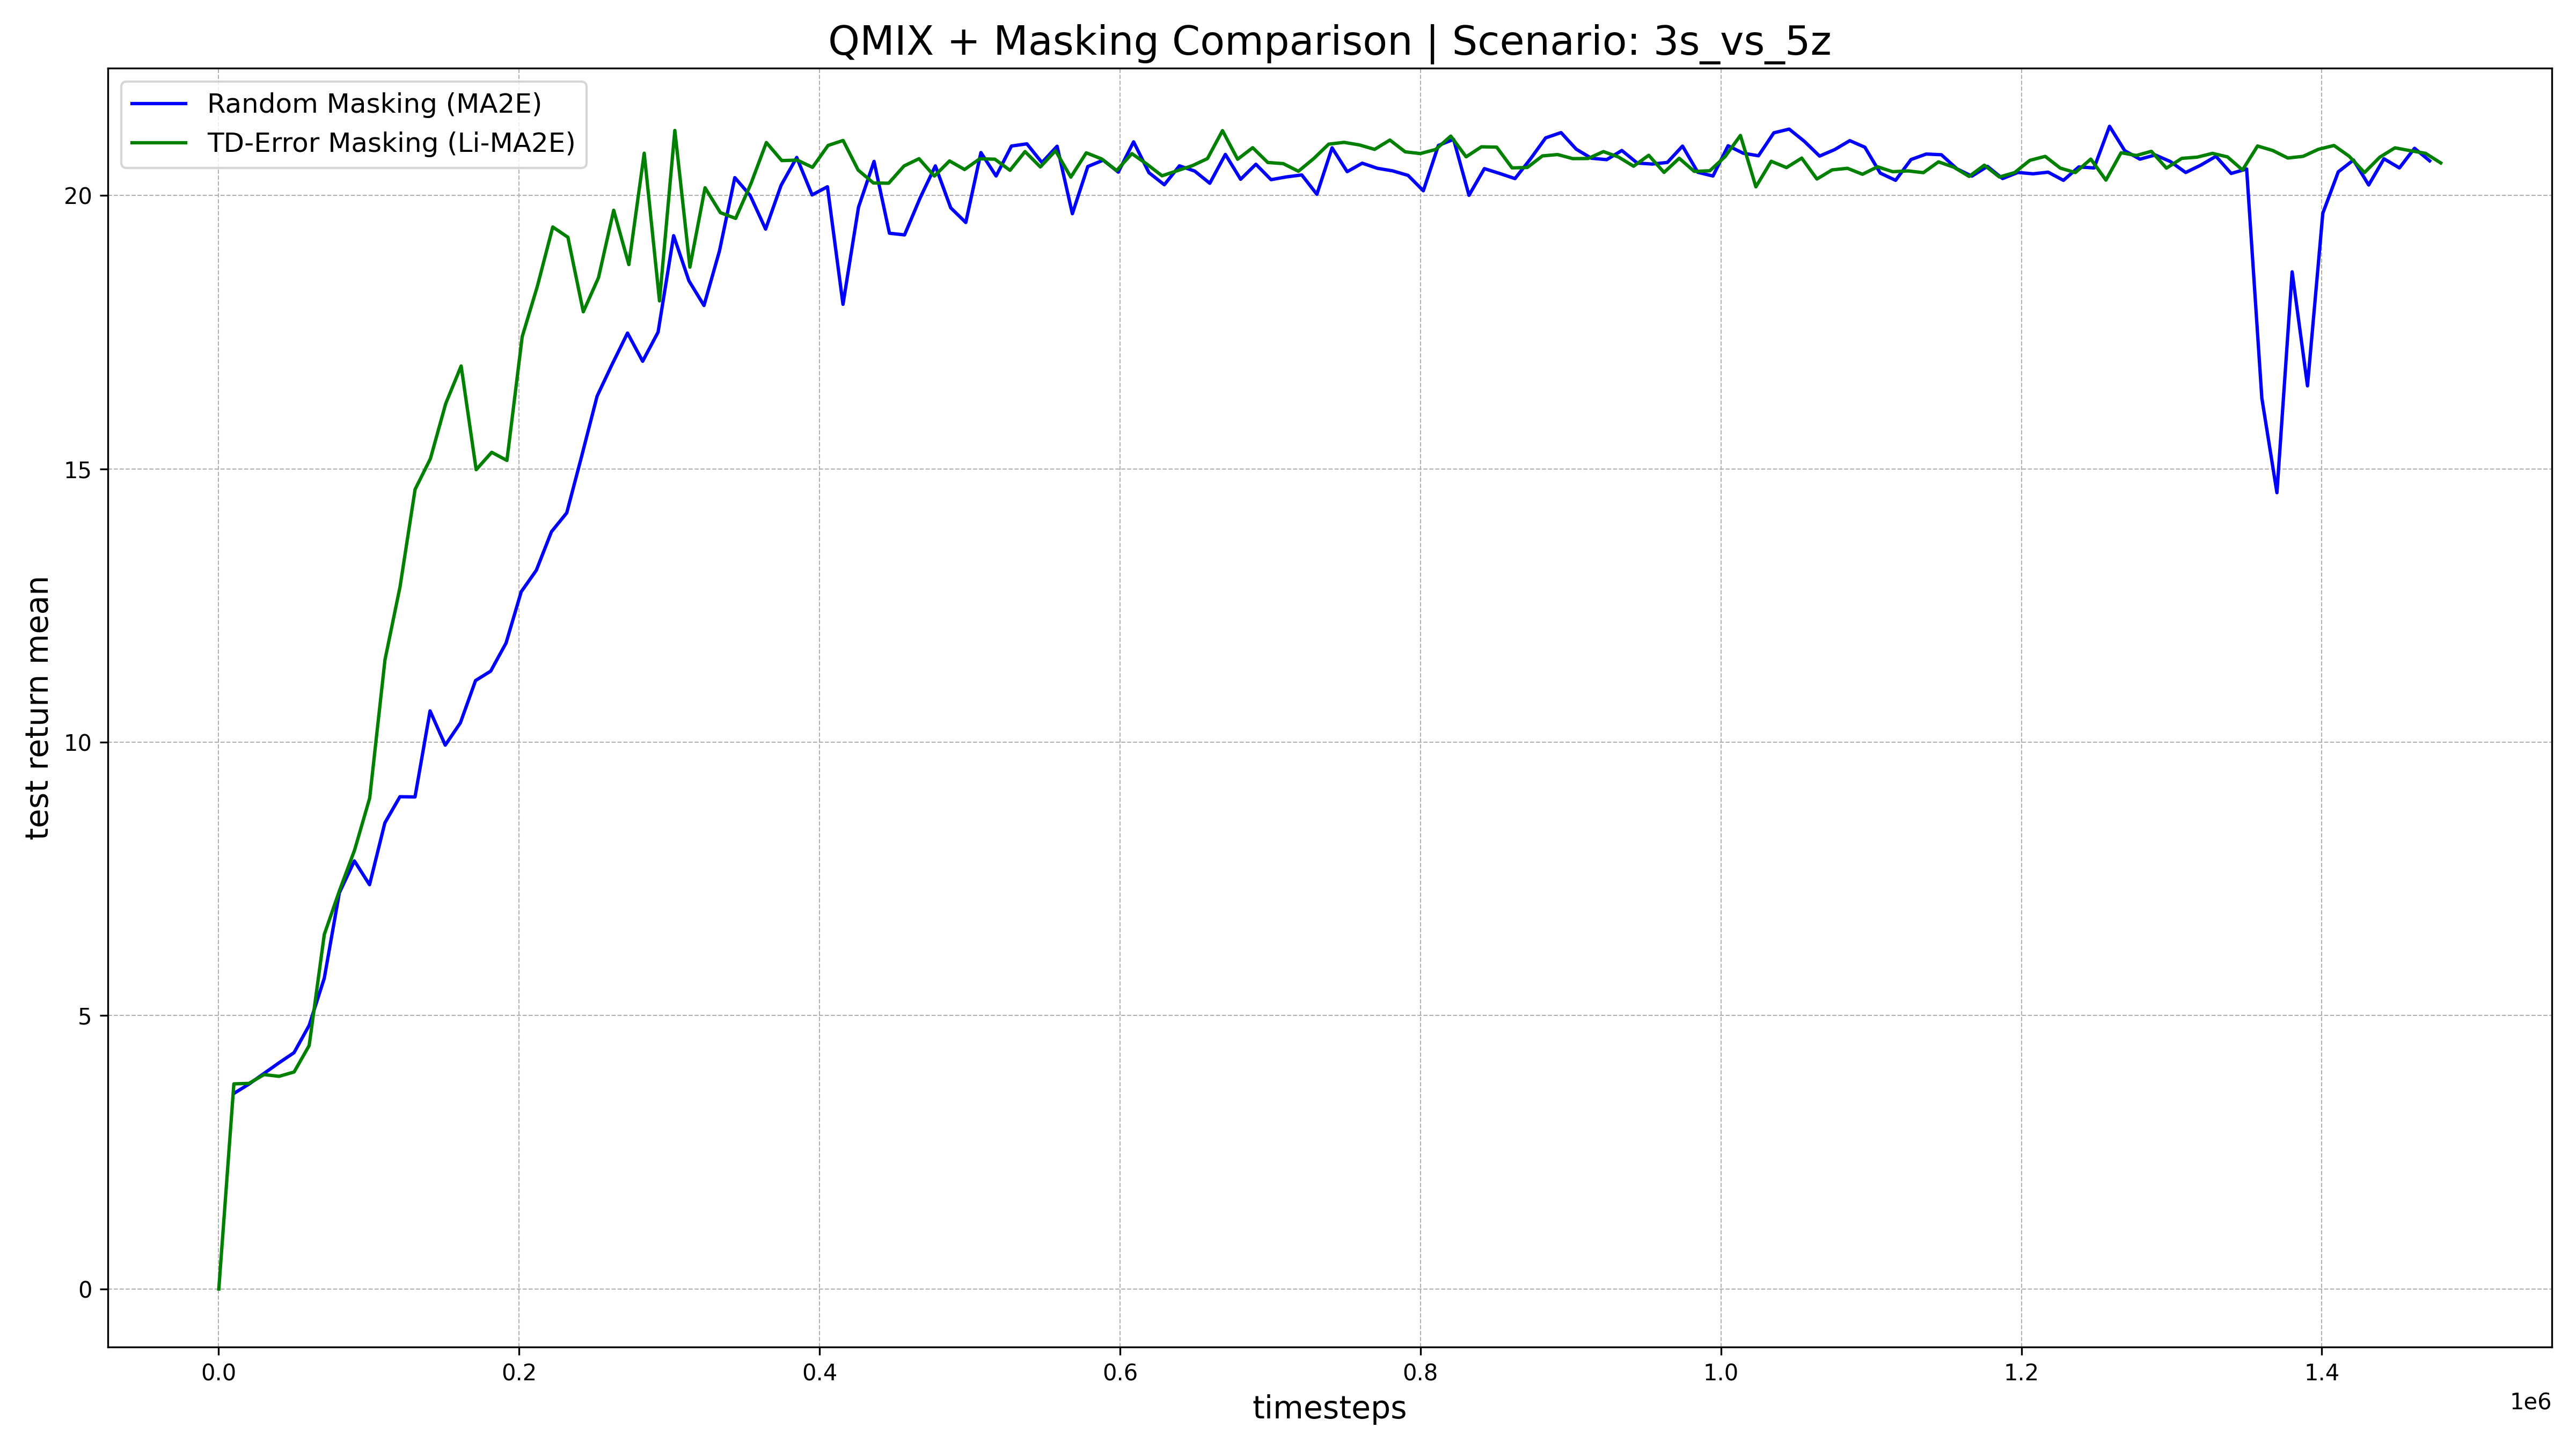
\includegraphics[width=0.32\textwidth]{images_pfe/results_test_return_mean/comparison_plot_3s_vs_5z.png}\label{fig:3s_vs_5z_return}}
    \hfill
    \subfloat[Scenario: 8m]{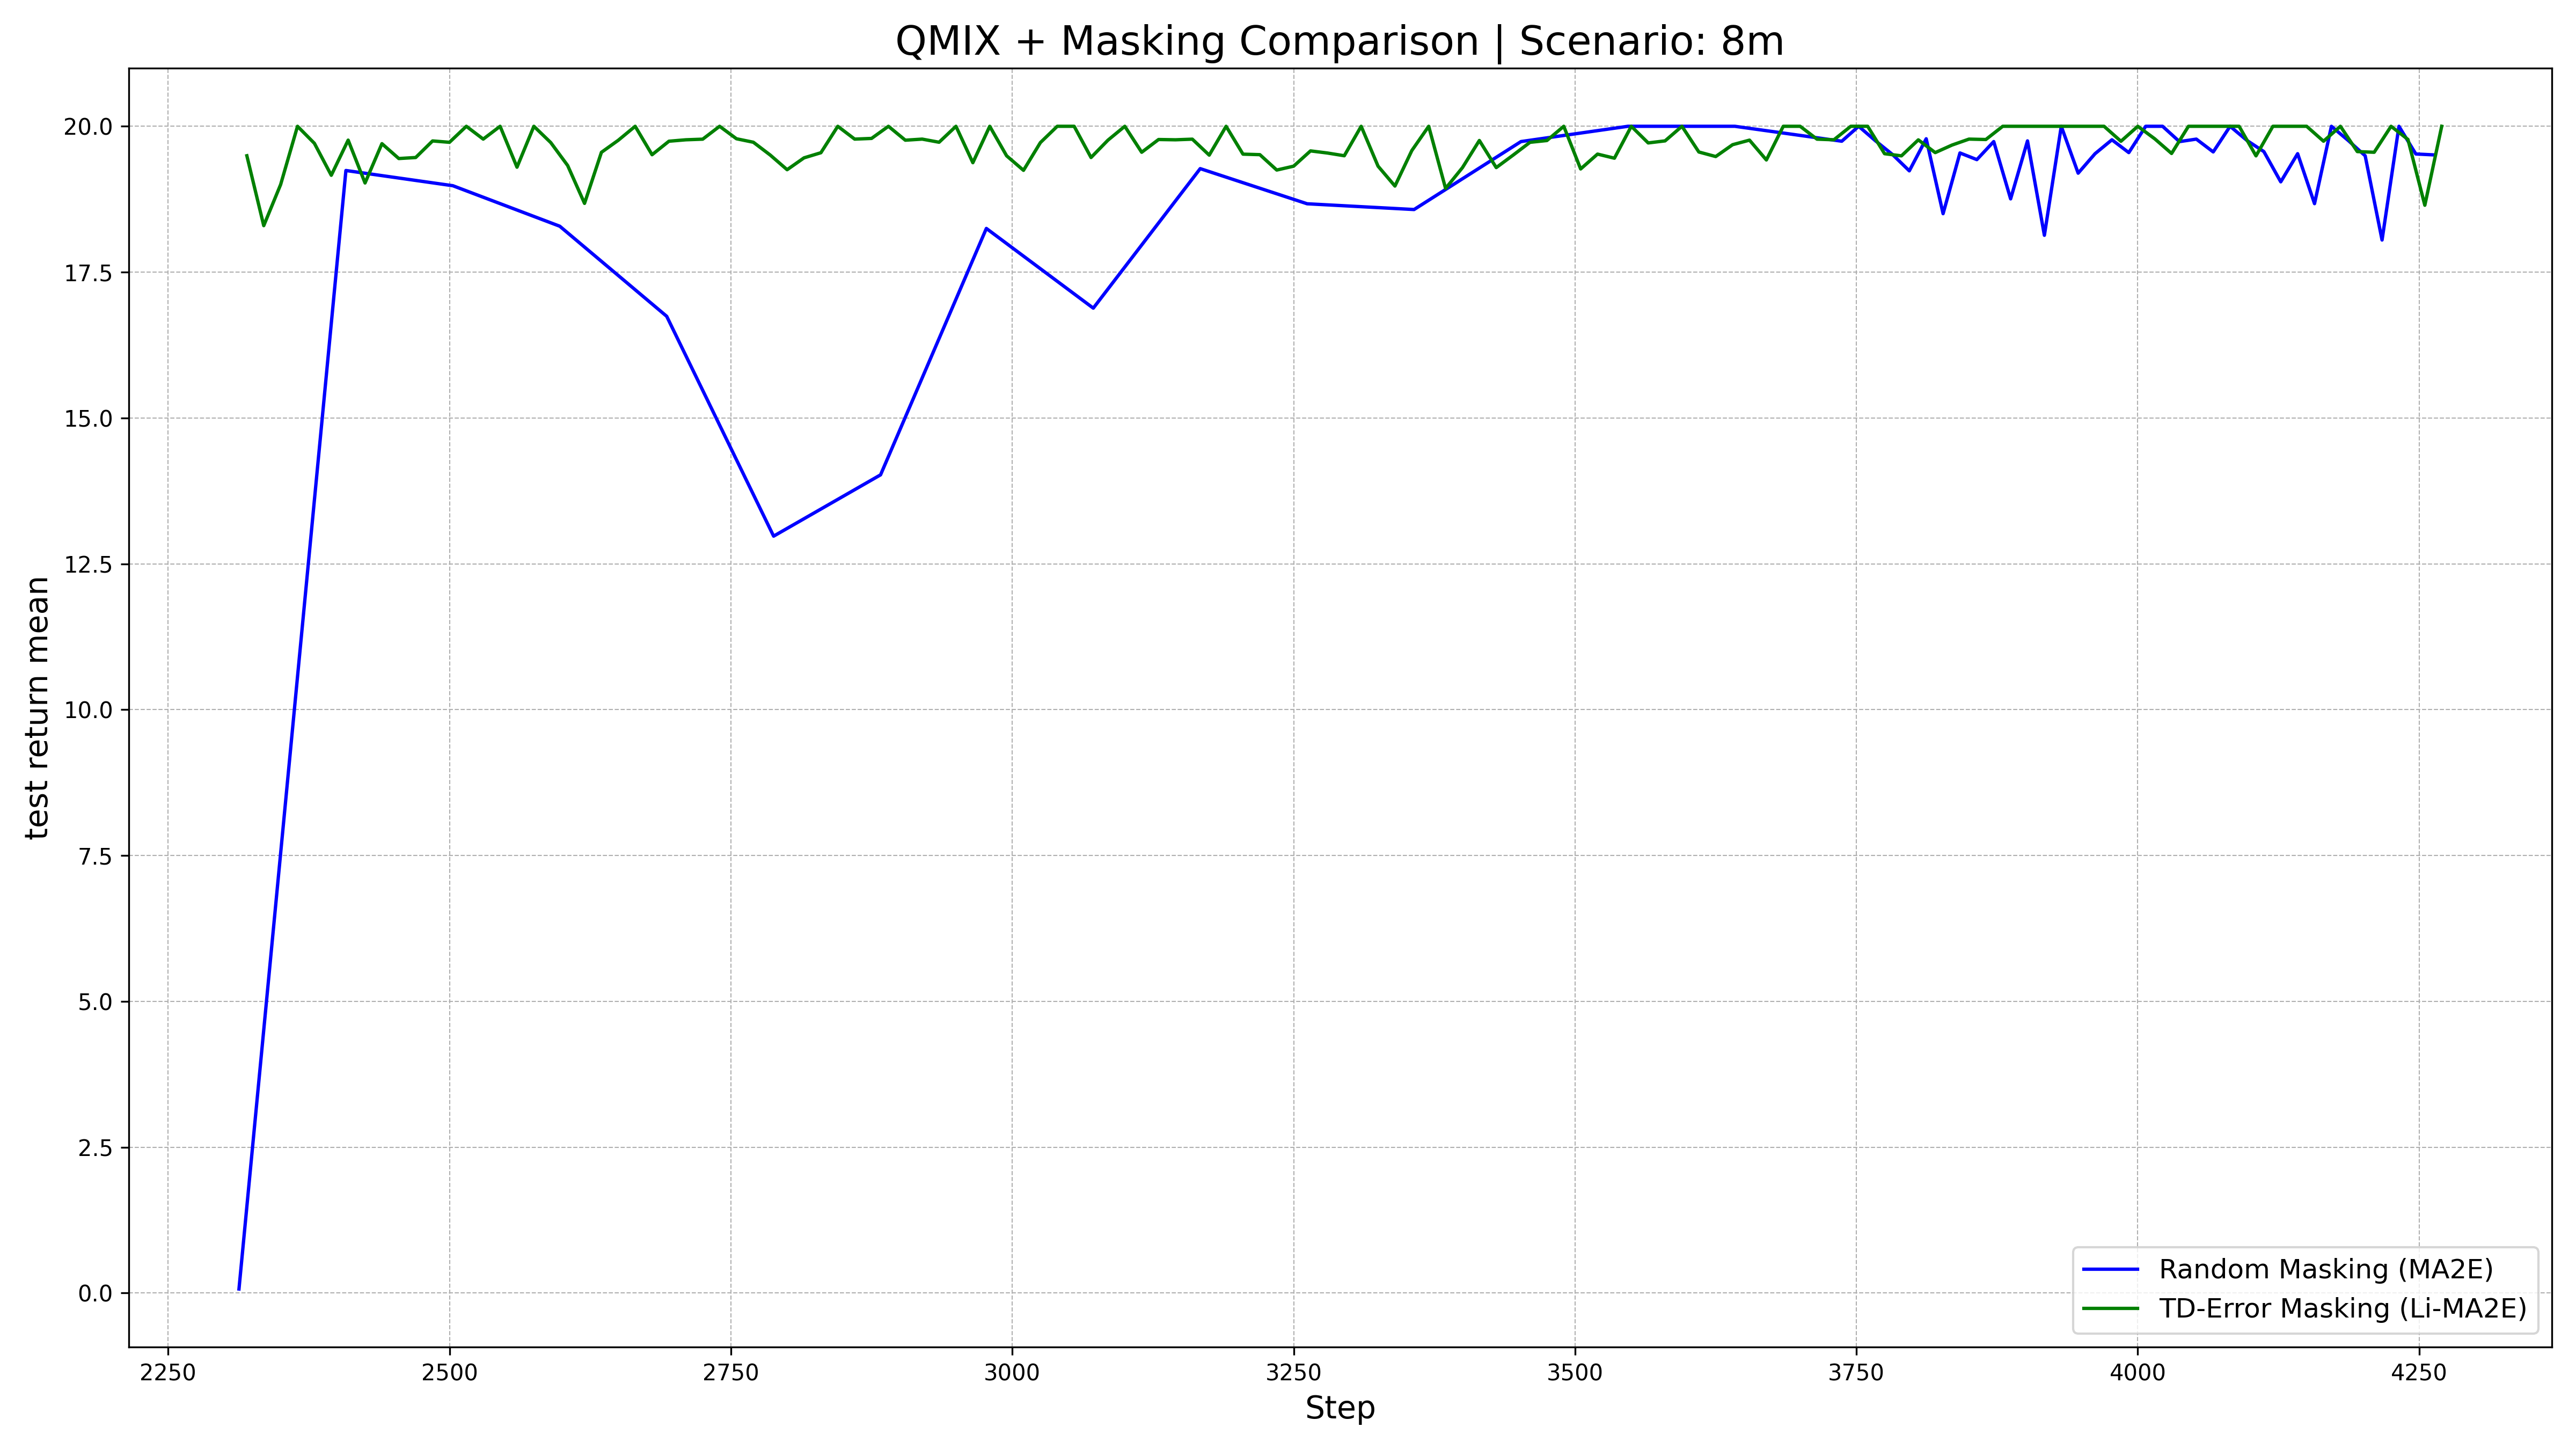
\includegraphics[width=0.32\textwidth]{images_pfe/results_test_return_mean/comparison_plot_8m.png}\label{fig:8m_return}}
    
    \caption{Mean test return for $LI-{MA}^2E$ (green) vs. baseline Random Masking (blue) across various SMAC scenarios. This metric shows the quality and efficiency of the learned policies.}
    \label{fig:all_returns}
\end{figure}
\paragraph{Analysis}
In scenarios such as \texttt{3s\_vs\_3z} and \texttt{3s\_vs\_4z}, our TD-Error Masking (green line) rapidly converges to the maximum possible return, while the baseline Random Masking (blue line) plateaus at a significantly lower, suboptimal level. Notably, in the \texttt{3s\_vs\_4z} scenario, while the baseline previously appeared to learn faster based on win rate, this more sensitive metric reveals that $LI-{MA}^2E$ learned the correct, high-reward strategy almost immediately, indicating a much higher policy quality. This advantage extends to the most difficult maps like \texttt{3s\_vs\_5z}, where  $LI-{MA}^2E$ not only achieves a higher return faster but also maintains a more stable final policy, avoiding the sharp performance drops exhibited by the baseline. Even on homogeneous maps like \texttt{3m} and \texttt{8m}, our method reaches the optimal return with greater speed and stability. Collectively, this strong evidence supports the conclusion that our intelligent masking strategy does not just help agents learn \textit{to} win, but guides them to learn \textit{how to win optimally}, producing more robust and efficient cooperative policies across a wide range of challenges.

\paragraph{Answer to RQ2:}
The evidence provides a decisive \textbf{yes}. Across all tested scenarios, the mean test return plots show that  $LI-{MA}^2E$ consistently learns higher-quality policies much more quickly than the baseline. 
\subsection{RQ3: What Are the Underlying Learning Dynamics?}
%----------------------------------------------------------------------------------------

\paragraph{Answer to RQ3 (Summary and Pointer to Appendix):}
The superior performance in both task completion and policy quality is a direct result of a more stable and efficient learning process. A detailed analysis of the underlying learning dynamics, presented in \textbf{Appendix~\ref{app:td_error_abs_analysis}}, directly addresses this question by examining the mean absolute TD-error. The analysis shows that our $LI-{MA}^2E$ framework is consistently more effective at reducing and stabilizing the agents' prediction errors, providing a mechanistic explanation for the observed performance gains.
\section*{Conclusion}

This chapter presented a comprehensive empirical validation of our proposed Learning-Informed Masking Framework. The experimental journey began with a methodical investigation into several candidate scoring functions, culminating in the selection of the \textbf{Adaptive Mean TD-Error Thresholding} strategy as the most robust and effective approach. The subsequent comparative analysis against the baseline framework provided strong empirical support for our central hypothesis. The results demonstrated that  $LI-{MA}^2E$ leads to more reliable \textbf{task completion (Win Rate)} and consistently produces \textbf{higher-quality and more efficient policies (Mean Test Return)}. The underlying mechanism for these improvements (a more stable and efficient learning process ) was substantiated by a direct analysis of the TD-error dynamics in the appendix. Collectively, the evidence confirms that an intelligent, learning-informed masking curriculum is superior to a random one, not only in achieving victory but in the quality and robustness of the strategies learned.

% \paragraph{Perspectives}
% The nuanced results from this chapter also open up several promising perspectives for future research. The varying performance of our method across different SMAC maps suggests that the optimal masking strategy may be scenario-dependent. A significant future direction would be to develop a meta-learning framework where the masking strategy itself (e.g., the choice of score or its hyperparameters) is adapted based on the detected characteristics of the environment. Furthermore, while TD-error proved to be a robust signal, future work could explore incorporating other information sources into the scoring function. Signals from credit assignment methods or even learned communication protocols could potentially provide an even richer, more context-aware metric for identifying the most critical agents to mask. These perspectives highlight how the principle of learning-informed masking can serve as a foundation for even more sophisticated and adaptive multi-agent learning systems.




